%% CUMCM-Master LaTeX 模板 — 2020 CUMCM C 题《中小微企业的信贷决策》
%% 编译方式：xelatex main.tex（运行两次以更新交叉引用）

\documentclass[12pt, a4paper]{article}

%% ======================== 宏包导入 ========================
\usepackage{ctex}                    % 中文支持
\usepackage[margin=2.5cm]{geometry}  % 页边距
\usepackage{amsmath, amssymb, amsthm}% 数学公式
\usepackage{graphicx}                % 插图
\usepackage{subcaption}              % 子图
\usepackage{booktabs}                % 三线表
\usepackage{longtable}               % 长表格
\usepackage{array}                   % 表格增强
\usepackage{multirow}                % 跨行单元格
\usepackage{float}                   % 浮动体控制 [H]
\usepackage{hyperref}                % 超链接
\usepackage{enumerate}               % 列表
\usepackage{enumitem}                % 列表定制
\usepackage{listings}                % 代码高亮
\usepackage{xcolor}                  % 颜色
\usepackage{tikz}                    % 流程图
\usepackage{pgfplots}                % 数据可视化
\usepackage{caption}                 % 标题定制
\usepackage{fancyhdr}                % 页眉页脚
\usepackage{setspace}                % 行距
\usepackage[numbers]{natbib}                  % 参考文献
\usepackage{appendix}                % 附录

\pgfplotsset{compat=1.18}
\usetikzlibrary{shapes.geometric, arrows.meta, positioning, calc}

%% ======================== 代码样式 ========================
\definecolor{codegray}{rgb}{0.5,0.5,0.5}
\definecolor{codepurple}{rgb}{0.58,0,0.82}
\definecolor{codeblue}{rgb}{0.13,0.29,0.53}
\definecolor{backcolour}{rgb}{0.97,0.97,0.97}

\lstdefinestyle{pythonstyle}{
    backgroundcolor=\color{backcolour},
    commentstyle=\color{codegray}\itshape,
    keywordstyle=\color{codeblue}\bfseries,
    stringstyle=\color{codepurple},
    basicstyle=\ttfamily\footnotesize,
    breakatwhitespace=false,
    breaklines=true,
    captionpos=b,
    keepspaces=true,
    numbers=left,
    numbersep=5pt,
    numberstyle=\tiny\color{codegray},
    showspaces=false,
    showstringspaces=false,
    showtabs=false,
    tabsize=4,
    frame=single,
    rulecolor=\color{black!20},
    language=Python
}

%% ======================== 页面样式 ========================
\pagestyle{fancy}
\fancyhf{}
\fancyhead[L]{\small 全国大学生数学建模竞赛}
\fancyhead[R]{\small \leftmark}
\fancyfoot[C]{\thepage}
\renewcommand{\headrulewidth}{0.4pt}
\setlength{\headheight}{14pt}

\captionsetup{font=small, labelfont=bf}
\setstretch{1.5}

%% ======================== 自定义命令 ========================
\newtheorem{assumption}{假设}[section]
\newtheorem{definition}{定义}[section]
\newtheorem{theorem}{定理}[section]

\newcommand{\prob}[1]{\mathbf{P}\left(#1\right)}
\newcommand{\E}[1]{\mathbb{E}\left[#1\right]}
\newcommand{\norm}[1]{\left\|#1\right\|}

%% ======================== 文档信息 ========================
\title{
    \vspace{-1cm}
    {\Large \textbf{中小微企业信贷风险量化与信贷策略优化}} \\[0.5em]
    {\large 全国大学生数学建模竞赛参赛论文（2020 CUMCM C 题）}
}
\author{}
\date{}

\begin{document}

\pagenumbering{arabic}
\setcounter{page}{1}

\maketitle
\thispagestyle{plain}

%% ---------------------- 摘要（电子版第 1 页）--------------
\begin{abstract}
\noindent
针对银行对中小微企业"评估信贷风险—确定放贷额度、利率"的决策问题，本文基于附件提供的约一百一十万条真实进销项发票记录，建立了"数据驱动风险量化 + 期望收益最大化分配"的信贷决策模型体系，并引入突发因素情景冲击建模给出调整策略。

\textbf{问题一}：对附件1的123家有信贷记录企业，从进销项发票中向量化聚合出36维经营特征（规模、活跃度、稳定性、集中度、作废/负数占比等），构建逻辑回归违约概率模型，5折交叉验证AUC达0.935（随机森林对照0.850），预测违约概率随信誉评级A、B、C、D单调递增（0.057/0.088/0.149/0.711），与银行专家评级Spearman相关系数0.645；同时以熵权-TOPSIS构建无标签客观评分轨交叉验证。在此基础上，结合附件3的利率-流失率曲线，对每家企业选择使期望收益最大的利率，并按"评级上限与25\%年销项额取小"设定额度上限，在年度信贷总额固定约束下按单位期望收益降序做线性背包分配，给出覆盖曲线（总额1亿元时放贷14家、期望收益352万元）。

\textbf{问题二}：将问题一校准的评分器迁移到附件2的302家无信贷记录企业，先用PSI检验分布偏移（关键金额特征轻度偏移、结构特征稳定），再按问题一各评级PD均值中点划分伪评级（A/B/C/D=141/38/81/42家），在1亿元总额下分配，放贷12家（均为A层级，平均利率4.7\%），实际分配恰为1亿元，期望收益356万元。

\textbf{问题三}：因企业名称脱敏、无行业字段，用发票行为特征KMeans聚类将302家企业分为4类行为画像（大型批发制造/高频小额零售餐饮/购销失衡贸易中介/大额低频项目工程，轮廓系数0.207），参照新冠疫情对不同行业的异质性影响文献设定情景冲击系数（零售餐饮0.35最高），以PD$'=\min\{\text{PD}(1+\delta_k),0.95\}$与销项额收缩传导冲击并重新分配1亿元，冲击后PD均值由0.188升至0.225，放贷12家中9家维持、2家收缩、1家加码，信贷资源向抗冲击能力强的低风险企业集中。

\textbf{灵敏度分析}：以tornado图考察6个关键参数，解对信贷总额与客户流失率假设较敏感（总额±2000万元使收益±66万元），对分层阈值、额度比例、冲击系数设定稳健，方向性结论可靠。全部模型均通过结构化自证验证（问题1/2/3验证报告分别为11/13/13项全通过），并为中小微企业信贷策略提供了一套可解释、可迁移、可情景化的决策工具。

\vspace{1em}
\noindent\textbf{关键词：}信贷风险量化；逻辑回归；熵权-TOPSIS；期望收益最大化分配；情景冲击分析；PSI迁移检验
\end{abstract}

\newpage

%% ==================== 1. 问题重述 ====================
\section{问题重述}

中小微企业规模小、缺乏抵押资产，银行通常依据信贷政策、企业交易票据信息与上下游影响力，对实力强、供求关系稳定的企业放贷，并对信誉高、风险小的企业给予利率优惠。某银行需依据附件数据制定信贷策略：对确定放贷企业，贷款额度以万元计，年利率在4\%至15\%之间，期限1年。

附件1给出123家有信贷记录企业的信誉评级（A/B/C/D）与是否违约标签及进销项发票明细；附件2给出302家无信贷记录企业的进销项发票明细；附件3给出2019年贷款年利率与客户流失率的统计关系（分A/B/C三档评级）。需要解决：

\begin{enumerate}[label=\textbf{问题\arabic*：}, leftmargin=*]
    \item 对附件1的123家企业进行信贷风险量化分析，给出银行在年度信贷总额固定时对这些企业的信贷策略；
    \item 在问题1基础上，对附件2的302家企业进行信贷风险量化分析，并给出年度信贷总额为1亿元时的信贷策略；
    \item 综合考虑附件2各企业信贷风险和突发因素（如新冠疫情）对不同类别企业的不同影响，给出年度信贷总额为1亿元时的信贷调整策略。
\end{enumerate}

%% ==================== 2. 问题背景与需要解决的问题 ====================
\section{问题背景与需要解决的问题}

\subsection{问题背景}

中小微企业是我国实体经济的重要组成，但受制于信息不对称与抵押物缺乏，长期面临融资难、融资贵的问题。银行在信贷决策中，需要在不掌握企业完整财务报表的情况下，仅凭交易票据等"软信息"评估企业真实经营状况与违约风险，进而在有限的年度信贷额度内实现收益与风险的平衡。发票数据作为企业购销活动的直接凭证，具有高频、真实、可审计的特点，为数据驱动的风险量化提供了良好基础。

\subsection{需要解决的问题}

本文需要解决的核心问题可归纳为"量化—分配—调整"三步。从决策科学角度看，该问题是一个在信息不对称（银行无法掌握企业完整财务信息）、资源有限（年度信贷总额固定）与外部不确定（突发因素）三重约束下的信贷组合决策问题：风险量化是前提，决定了"哪些企业值得贷"；额度与利率是手段，决定了"贷多少、以什么价格贷"；情景调整是保障，决定了"外部冲击来临时如何动态应对"。三问层层递进：首先从发票数据量化每家企业的信贷风险（违约概率），其次在年度信贷总额约束下确定放贷对象、额度与利率以最大化期望收益，最后将突发因素对不同类别企业的异质性冲击纳入模型，给出动态调整策略。三个问题层层递进：问题一利用有标签样本建立可解释的风险量化模型并给出一般性分配策略；问题二将模型迁移到无标签样本并给出1亿元额度下的具体策略；问题三在问题二基础上叠加突发因素冲击，考察策略的稳健性与调整方向。

%% ==================== 3. 问题分析 ====================
\section{问题分析}

本文按"特征工程—风险量化—策略优化—冲击调整"的总体思路建模，整体流程如图~\ref{fig:pipeline}~所示。

\begin{figure}[H]
\centering
\begin{tikzpicture}[
    box/.style={rectangle, rounded corners, draw=black, fill=blue!10,
                text width=2.6cm, align=center, minimum height=0.75cm, font=\small},
    arrow/.style={-Stealth, thick}
]
    \node[box] (f)  {发票数据\\向量化特征工程};
    \node[box, right=0.9cm of f] (r) {逻辑回归\\违约概率(PD)};
    \node[box, right=0.9cm of r] (s) {利率-流失率权衡\\期望收益最大化};
    \node[box, right=0.9cm of s] (a) {总额约束下\\信贷分配};
    \node[box, below=0.8cm of a] (sh) {突发因素\\情景冲击};
    \node[box, below=0.8cm of sh] (adj) {信贷调整\\策略};
    \draw[arrow] (f) -- (r);
    \draw[arrow] (r) -- (s);
    \draw[arrow] (s) -- (a);
    \draw[arrow] (a) -- (sh);
    \draw[arrow] (sh) -- (adj);
    \draw[arrow] (a) -- node[right, font=\scriptsize]{问题2} (sh);
    \draw[arrow] (r) -- node[above, font=\scriptsize]{迁移打分} ([yshift=0.35cm]f.west);
\end{tikzpicture}
\caption{总体建模流程}
\label{fig:pipeline}
\end{figure}

\subsection{问题一分析}

问题一属于\textbf{监督分类与资源分配}的混合问题，其难点有二。其一，银行掌握的并非财务报表，而是海量、非结构化的交易票据，需要从中提炼能稳定区分违约与正常企业的特征；其二，信贷策略是"给谁贷、贷多少、定多高利率"的联合决策，且必须在年度总额约束下全局最优。附件1提供了"是否违约"的监督标签与信誉评级，可将风险量化建模为二分类任务：从进销项发票中提取反映企业经营规模、购销稳定性、票据质量与上下游结构的特征，训练可输出概率的逻辑回归模型得到违约概率PD，并以熵权-TOPSIS无标签评分轨交叉验证。信贷策略方面，利率的选取需同时权衡利息收入与客户流失（附件3给出二者关系），而额度分配则在"总额固定"约束下以期望收益最大化为目标，构成带容量约束的线性背包问题，可按单位期望收益降序的贪心法求得最优解。

\subsection{问题二分析}

问题二的核心困难是附件2企业\textbf{没有信誉评级与违约标签}，无法直接套用问题一的监督信号与附件3的分档流失率曲线。处理思路是迁移学习：问题一建立的评分器仅依赖发票特征（不含评级），可直接对附件2打分，但迁移成立的前提是两样本特征分布相近——这需要先用PSI（群体稳定性指数）量化检验，对发生明显偏移的特征在解释结论时予以限定。打分完成后，再依据问题一各评级PD分布的均值中点将302家企业映射为伪评级，从而沿用利率-流失率曲线、额度上限与D级不放贷规则，在1亿元约束下做同样的期望收益最大化分配。

\subsection{问题三分析}

问题三要求刻画突发因素对不同类别企业的异质性影响，其特殊性在于：突发因素（如新冠疫情）没有历史数据可循，只能以\textbf{情景分析}方式处理；且企业名称已脱敏、数据中没有行业字段，无法直接按行业划分受影响程度。本文的解法是：先用发票行为特征（规模、频次、票额、进销比等）对附件2企业做KMeans聚类，得到可解释的行为类别画像（高频小额零售餐饮型、大型批发制造型等），再参照新冠疫情冲击下分行业信用压力的文献结论为各类别设定情景冲击系数，通过PD乘子与销项额收缩两种渠道传导冲击，重新求解1亿元下的最优分配，与基线对比得到"维持/收缩/加码"调整动作。该情景框架将"突发因素"从定性描述转化为可量化的压力测试参数，便于银行在冲击情景间做预案切换。

%% ==================== 4. 模型假设 ====================
\section{模型假设}

为使模型具有可操作性，结合题目实际背景，本文提出以下假设：

\begin{enumerate}[label=\textbf{假设\arabic*：}, leftmargin=*]
    \item 发票数据真实反映企业购销活动，且观测窗口（2016年10月至2020年2月）内的经营行为对违约风险具有代表性。\\
          \textit{依据：}发票由税务系统开具，造假成本高；观测窗口覆盖41个月，足以刻画稳定经营状态。

    \item 企业一旦违约，银行损失为未回收本金，即回收率$R=0$。\\
          \textit{依据：}题目明确中小微企业"缺少抵押资产"，故按全额损失保守估计；灵敏度分析中考察$R=0.4$的情形。

    \item 附件3的利率-流失率曲线对两类样本均适用，且可由离散统计点线性插值到任意利率。\\
          \textit{依据：}2019年统计数据，曲线单调递增且平滑；问题二以伪评级套用对应档位曲线。

    \item 附件2与附件1企业来自同一银行信贷评估体系，特征分布偏移程度可用PSI量化，且轻中度偏移下迁移打分仍然有效。\\
          \textit{依据：}两附件发票字段、窗口完全一致；PSI检验显示结构特征稳定。

    \item 突发因素对企业的冲击强度仅与行为类别相关，且可量化为对违约概率的乘子$\delta_k$与对销项额的收缩比例。\\
          \textit{依据：}文献表明疫情对住宿餐饮、零售等服务类冲击显著大于制造类；本文以行为类别代理行业。

    \item 银行按年计息、单利计息，贷款期限统一为1年，不存在提前还款与额度转贷。\\
          \textit{依据：}题目给定期限1年，简化计息不改变策略排序。

    \item 企业在给定利率下接受贷款的概率为$1-c_k(r)$（$c_k$为客户流失率），且相互独立。\\
          \textit{依据：}流失率定义即"因贷款利率等因素失去潜在客户的比率"，本文取其互补为接受贷款概率。
\end{enumerate}

%% ==================== 5. 符号说明 ====================
\section{符号说明}

本文所用主要符号及其含义如表~\ref{tab:symbols}~所示。

\begin{table}[H]
\centering
\caption{主要符号说明}
\label{tab:symbols}
\begin{tabular}{cll}
\toprule
\textbf{符号} & \textbf{含义} & \textbf{单位/量纲} \\
\midrule
$\mathrm{PD}_i$ & 企业$i$的违约概率 & 无量纲 \\
$X_i$   & 企业$i$的发票特征向量 & — \\
$\boldsymbol{\beta}$ & 逻辑回归系数 & — \\
$r_i$   & 企业$i$的贷款年利率 & 无量纲（4\%--15\%） \\
$c_k(r)$ & 评级/层级$k$在利率$r$下的客户流失率 & 无量纲 \\
$A_i$   & 企业$i$的贷款额度 & 万元 \\
$S_i$   & 企业$i$的年销项金额 & 万元 \\
$\theta$ & 额度上限占年销项额比例 & 无量纲（0.25） \\
$C_k$   & 评级/层级$k$的额度上限 & 万元 \\
$\pi_i(r)$ & 企业$i$在利率$r$下的单位额度期望收益 & 无量纲 \\
$T$     & 年度信贷总额 & 万元 \\
$\delta_k$ & 类别$k$的突发因素冲击系数 & 无量纲 \\
$n$     & 企业数量 & 个 \\
\bottomrule
\end{tabular}
\end{table}

%% ==================== 6. 模型的建立与求解 ====================
\section{模型的建立与求解}

\subsection{问题一：信贷风险量化与总额固定下的信贷策略}

\subsubsection{特征工程}

附件1进项发票210\,947行、销项发票162\,484行，附件2进项发票395\,175行、销项发票330\,835行，合计约110万行，金额字段无缺失，观测窗口统一为2016年10月至2020年2月（41个月），企业代号在两附件内均唯一。对每家企业，按进项、销项两个方向分别做向量化聚合（\texttt{groupby}+\texttt{agg}，避免逐行循环），构造36维经营特征，覆盖四类信息：\textbf{规模类}（发票数量、金额合计、净额、税额合计、单票平均与最大金额）、\textbf{票据质量类}（作废发票占比、负数发票占比、税率代理）、\textbf{购销结构类}（对手方数量、对手方集中度HHI、进销比$S_{\text{out}}/S_{\text{in}}$）以及\textbf{经营稳定性类}（活跃月份数、月度金额变异系数、月度增长趋势、月均发票强度）。

附件1中违约率随信誉评级严格单调（A:0\%、B:2.6\%、C:5.9\%、D:100\%，图~\ref{fig:default_by_rating}），说明评级蕴含强风险信息，但评级属人工评定且附件2缺失，故主模型仅使用发票特征以保证可迁移性，评级留作交叉验证。图~\ref{fig:corr_heatmap}为特征相关性热力图，可见规模类特征高度相关，模型采用L2正则化处理多重共线性。

\begin{figure}[H]
    \centering
    \begin{minipage}[t]{0.46\textwidth}
        \centering
        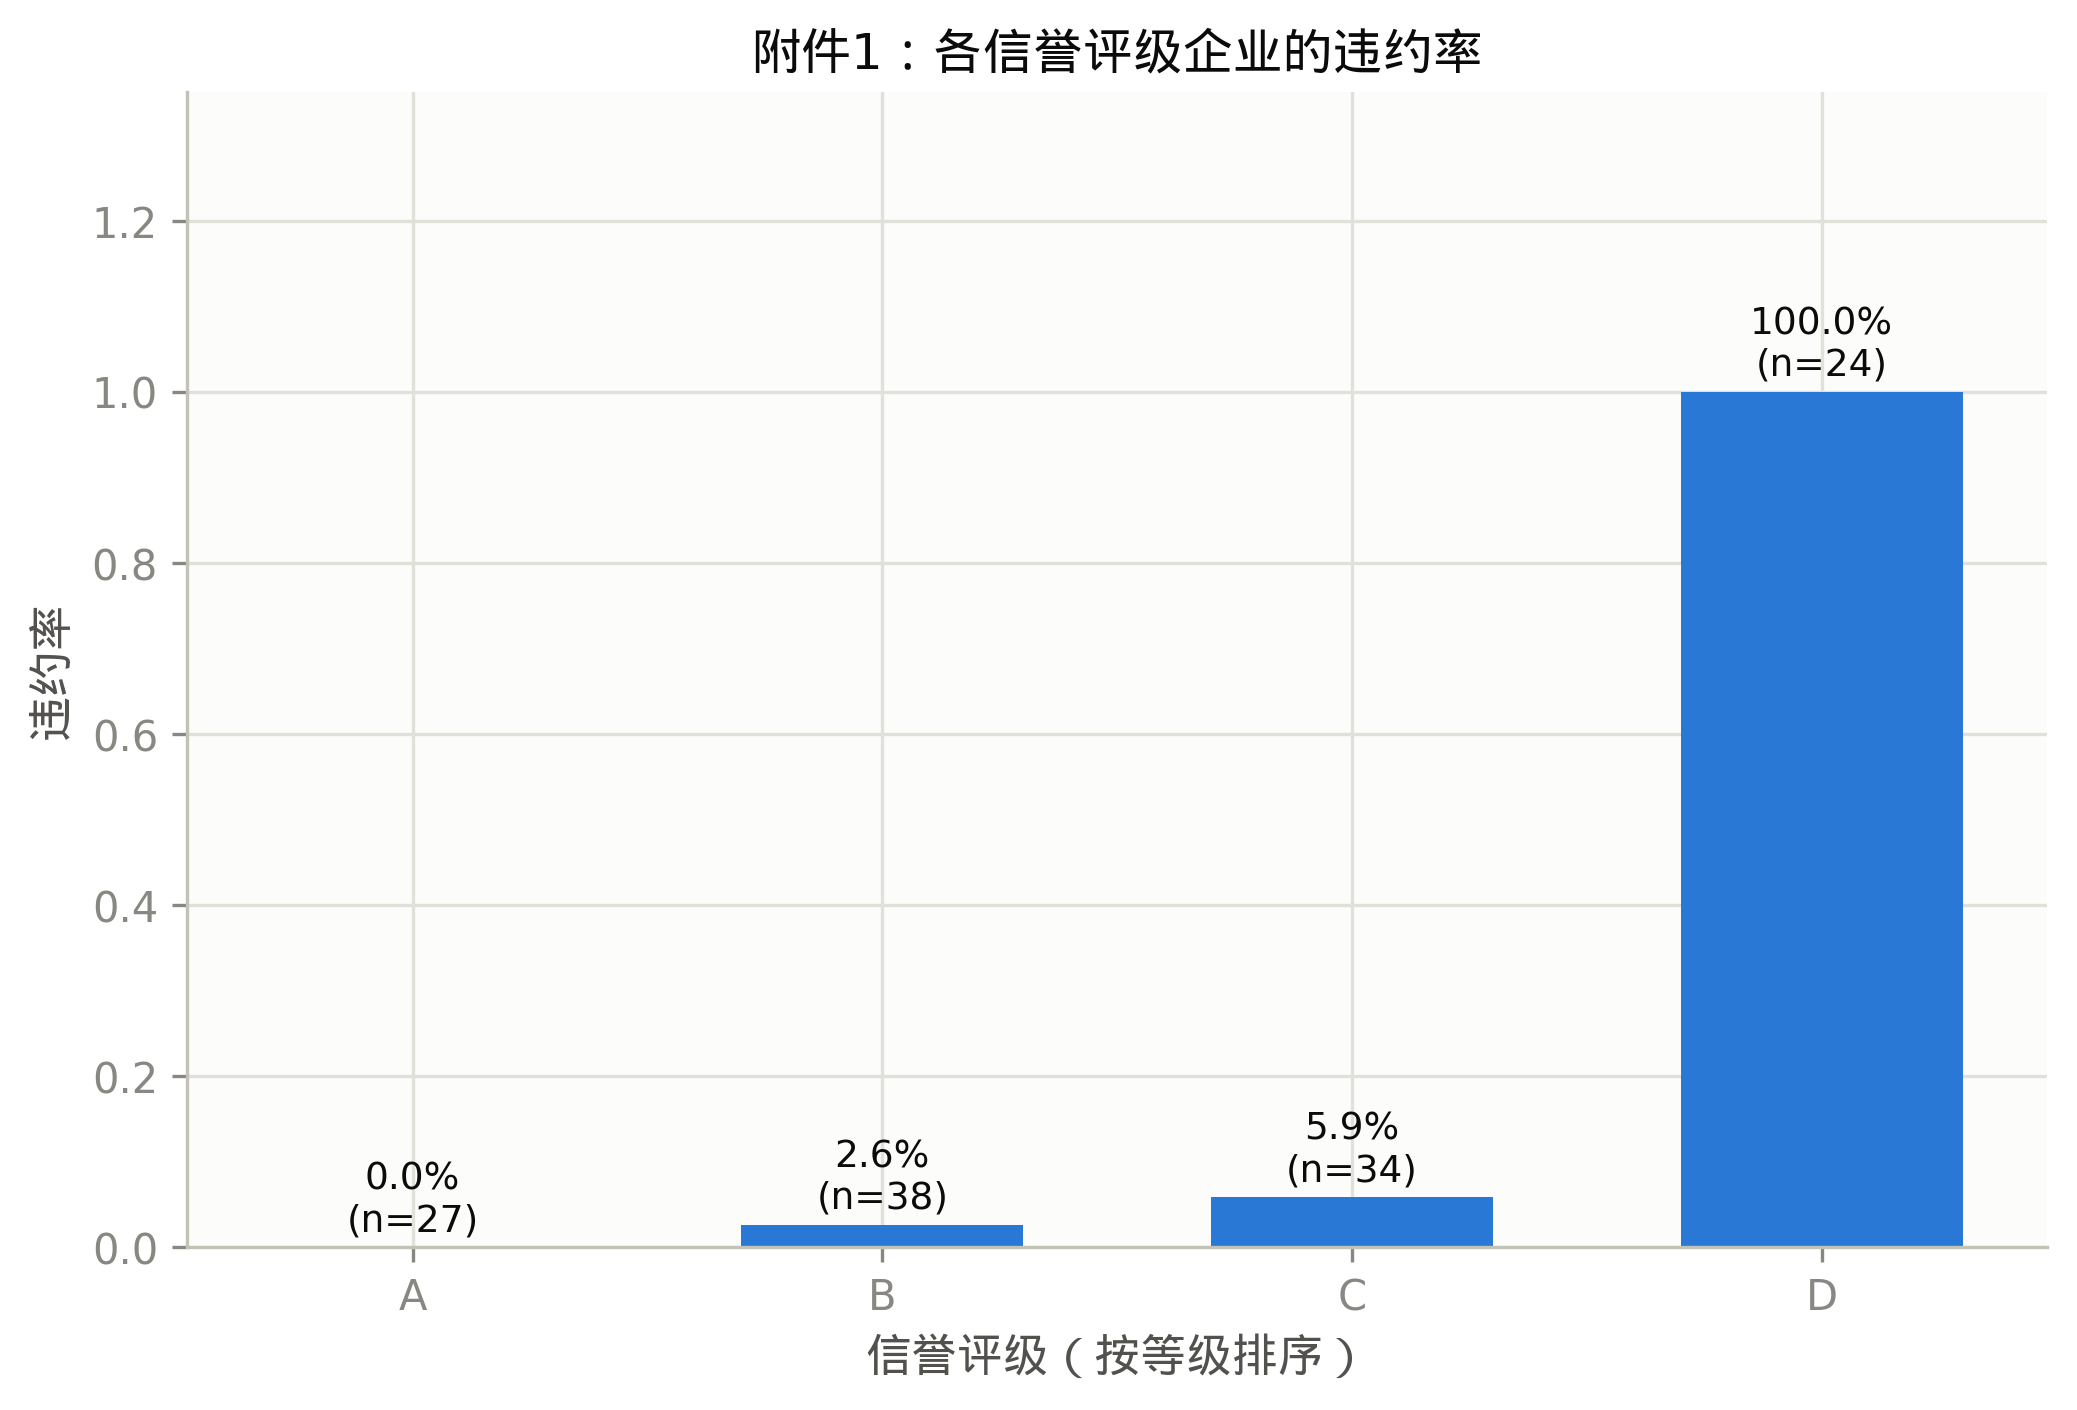
\includegraphics[width=\textwidth]{images/fig00_01_default_rate_by_rating.png}
        \caption{附件1各信誉评级违约率}
        \label{fig:default_by_rating}
    \end{minipage}
    \hfill
    \begin{minipage}[t]{0.52\textwidth}
        \centering
        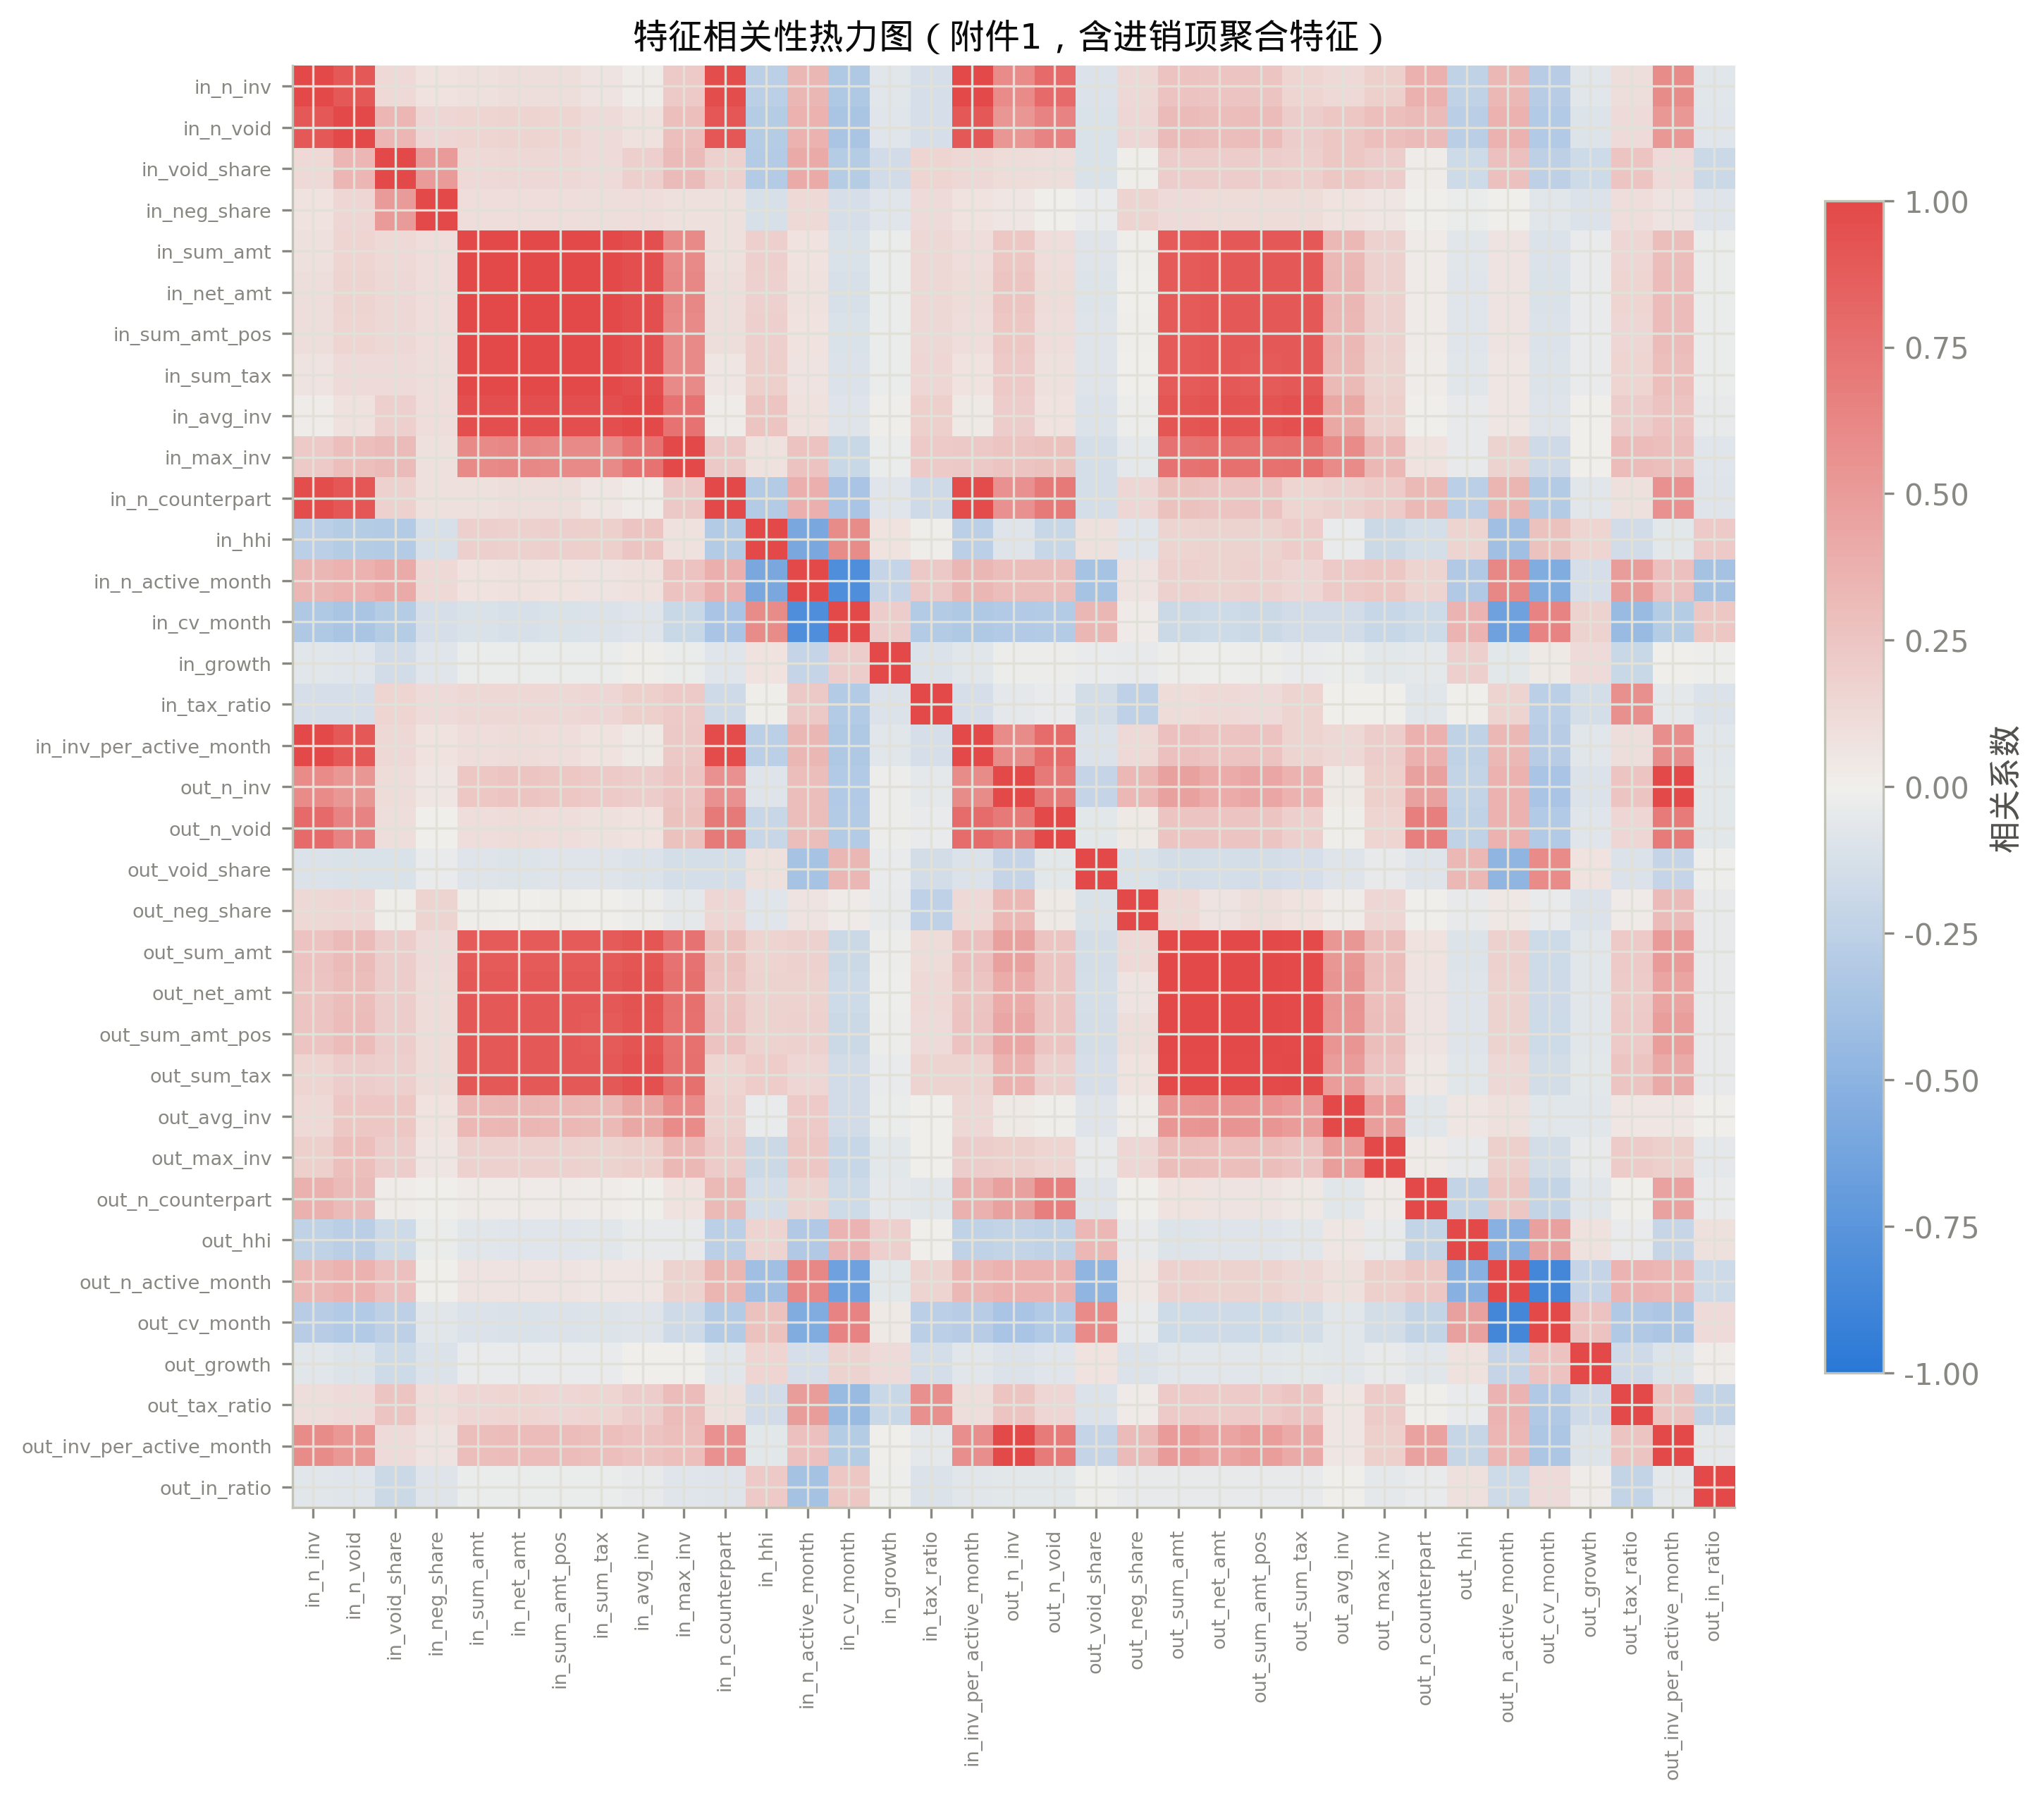
\includegraphics[width=\textwidth]{images/fig00_02_feature_corr_heatmap.png}
        \caption{特征相关性热力图}
        \label{fig:corr_heatmap}
    \end{minipage}
\end{figure}

\subsubsection{违约概率模型}

对金额、数量类特征做$\log(1+x)$变换消除量纲偏态，再标准化。逻辑回归是中小企业信用风险评估的经典方法\cite{Fahr2022}，相比神经网络类方法\cite{Chen2024}虽判别力略逊，但系数可直接解释、输出天然为概率，且在小样本下更稳健，故作为主模型。以$y_i\in\{0,1\}$表示是否违约，逻辑回归假设：
\begin{equation}
    \prob{y_i=1\mid X_i} = \frac{1}{1+\exp\left[-\left(\beta_0+\boldsymbol{\beta}^{\mathsf{T}}\tilde{X}_i\right)\right]},
    \label{eq:lr}
\end{equation}

其中$\tilde{X}_i$为变换标准化后的特征向量。模型以5折分层交叉验证的AUC为目标，在$\{0.05,0.1,0.3,1,3\}$网格上搜索正则化强度$C$，最优$C=0.10$；同时训练随机森林作对照。

\begin{table}[H]
\centering
\caption{问题一违约概率模型评估}
\label{tab:p1_model}
\begin{tabular}{ccc}
\toprule
\textbf{指标} & \textbf{逻辑回归（主）} & \textbf{随机森林（对照）} \\
\midrule
5折CV AUC & $0.9351\pm0.0550$ & $0.8501\pm0.1096$ \\
预测PD均值（A/B/C/D） & 0.057/0.088/0.149/0.711 & — \\
PD与评级等级 Spearman $\rho$ & $0.6454$ & — \\
\bottomrule
\end{tabular}
\end{table}

如表~\ref{tab:p1_model}~所示，逻辑回归AUC达0.935，显著优于随机森林的0.850。同时，预测PD随评级严格单调（图~\ref{fig:pd_by_rating}），与银行专家评级高度一致（Spearman $\rho=0.645$），说明模型从发票特征中有效学习到了风险结构。图~\ref{fig:risk_heatmap}为123家企业按预测风险分为10个十分位、箱内取均值的风险画像热力图——这是信用风险评估领域的标准呈现方式\cite{Dickson2011}，分箱处理也让格子比例保持方正、避免123家企业逐一展开导致的窄条畸变——可直观看到高风险十分位（图右侧）在作废率、负数占比与变异系数上明显偏高。作为无标签场景的交叉验证轨，熵权-TOPSIS客观评分与$-\text{PD}$的Spearman相关仅$\rho=-0.04$，表明纯无监督综合评分在不借助违约标签时判别力有限，佐证了以监督模型为主、TOPSIS为辅的双轨设计。

从逻辑回归标准化系数（表~\ref{tab:coef}）可解读风险驱动因素：\textbf{风险升高端}为销项月度变异系数（0.47）、进/销项税率代理（0.41/0.28）、销项作废率（0.27）与客户集中度HHI（0.18），说明经营波动大、票据质量差、税率结构异常、销售依赖少数客户的企业违约风险高；\textbf{风险降低端}为供应商集中度（$-0.28$）与销项规模、活跃月数，说明供应链稳定、购销规模大、经营持续的企业风险低。这些发现与信贷实务直觉一致，增强了模型的可解释性。

\begin{table}[H]
\centering
\caption{逻辑回归标准化系数：风险驱动因素解读（取绝对值最大的各5项）}
\label{tab:coef}
{\small
\begin{tabular}{llll}
\toprule
\textbf{风险升高（正系数）} & \textbf{系数} & \textbf{风险降低（负系数）} & \textbf{系数} \\
\midrule
销项月度变异系数 out\_cv\_month & 0.465 & 供应商集中度 in\_hhi & $-0.276$ \\
进项税率代理 in\_tax\_ratio & 0.409 & 销项净额 out\_net\_amt & $-0.261$ \\
销项税率代理 out\_tax\_ratio & 0.285 & 销项金额合计 out\_sum\_amt\_pos & $-0.253$ \\
销项作废率 out\_void\_share & 0.273 & 销项金额合计 out\_sum\_amt & $-0.250$ \\
客户集中度 out\_hhi & 0.185 & 单票平均金额 out\_avg\_inv & $-0.233$ \\
\bottomrule
\end{tabular}}
\end{table}

\begin{figure}[H]
    \centering
    \begin{minipage}[t]{0.46\textwidth}
        \centering
        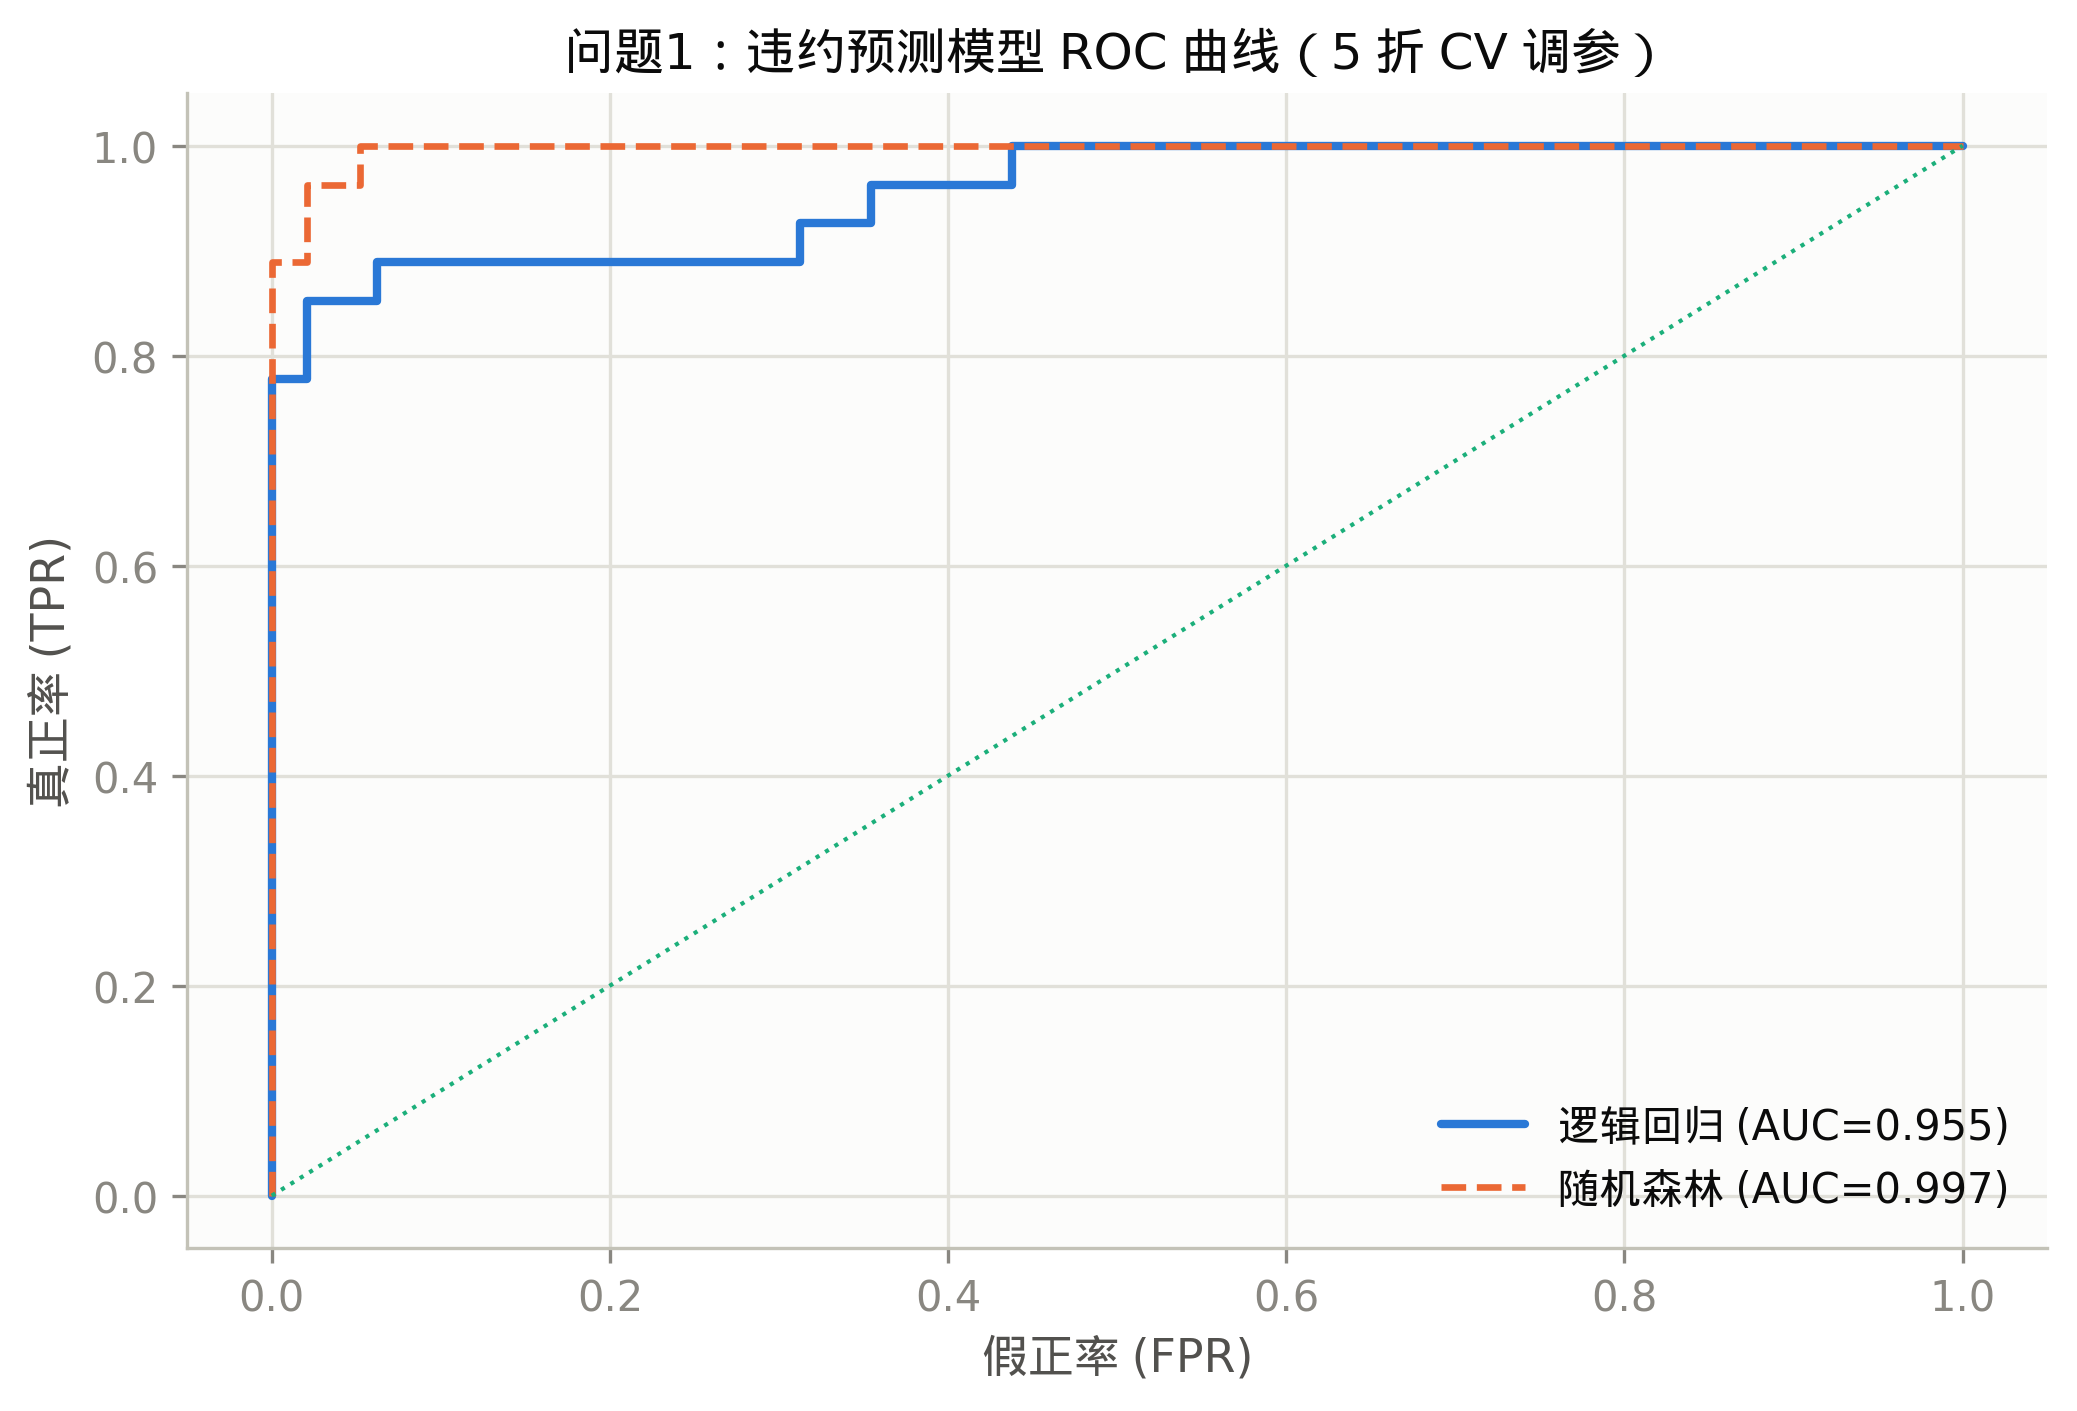
\includegraphics[width=\textwidth]{images/fig10_01_roc_curve.png}
        \caption{ROC曲线}
        \label{fig:roc}
    \end{minipage}
    \hfill
    \begin{minipage}[t]{0.52\textwidth}
        \centering
        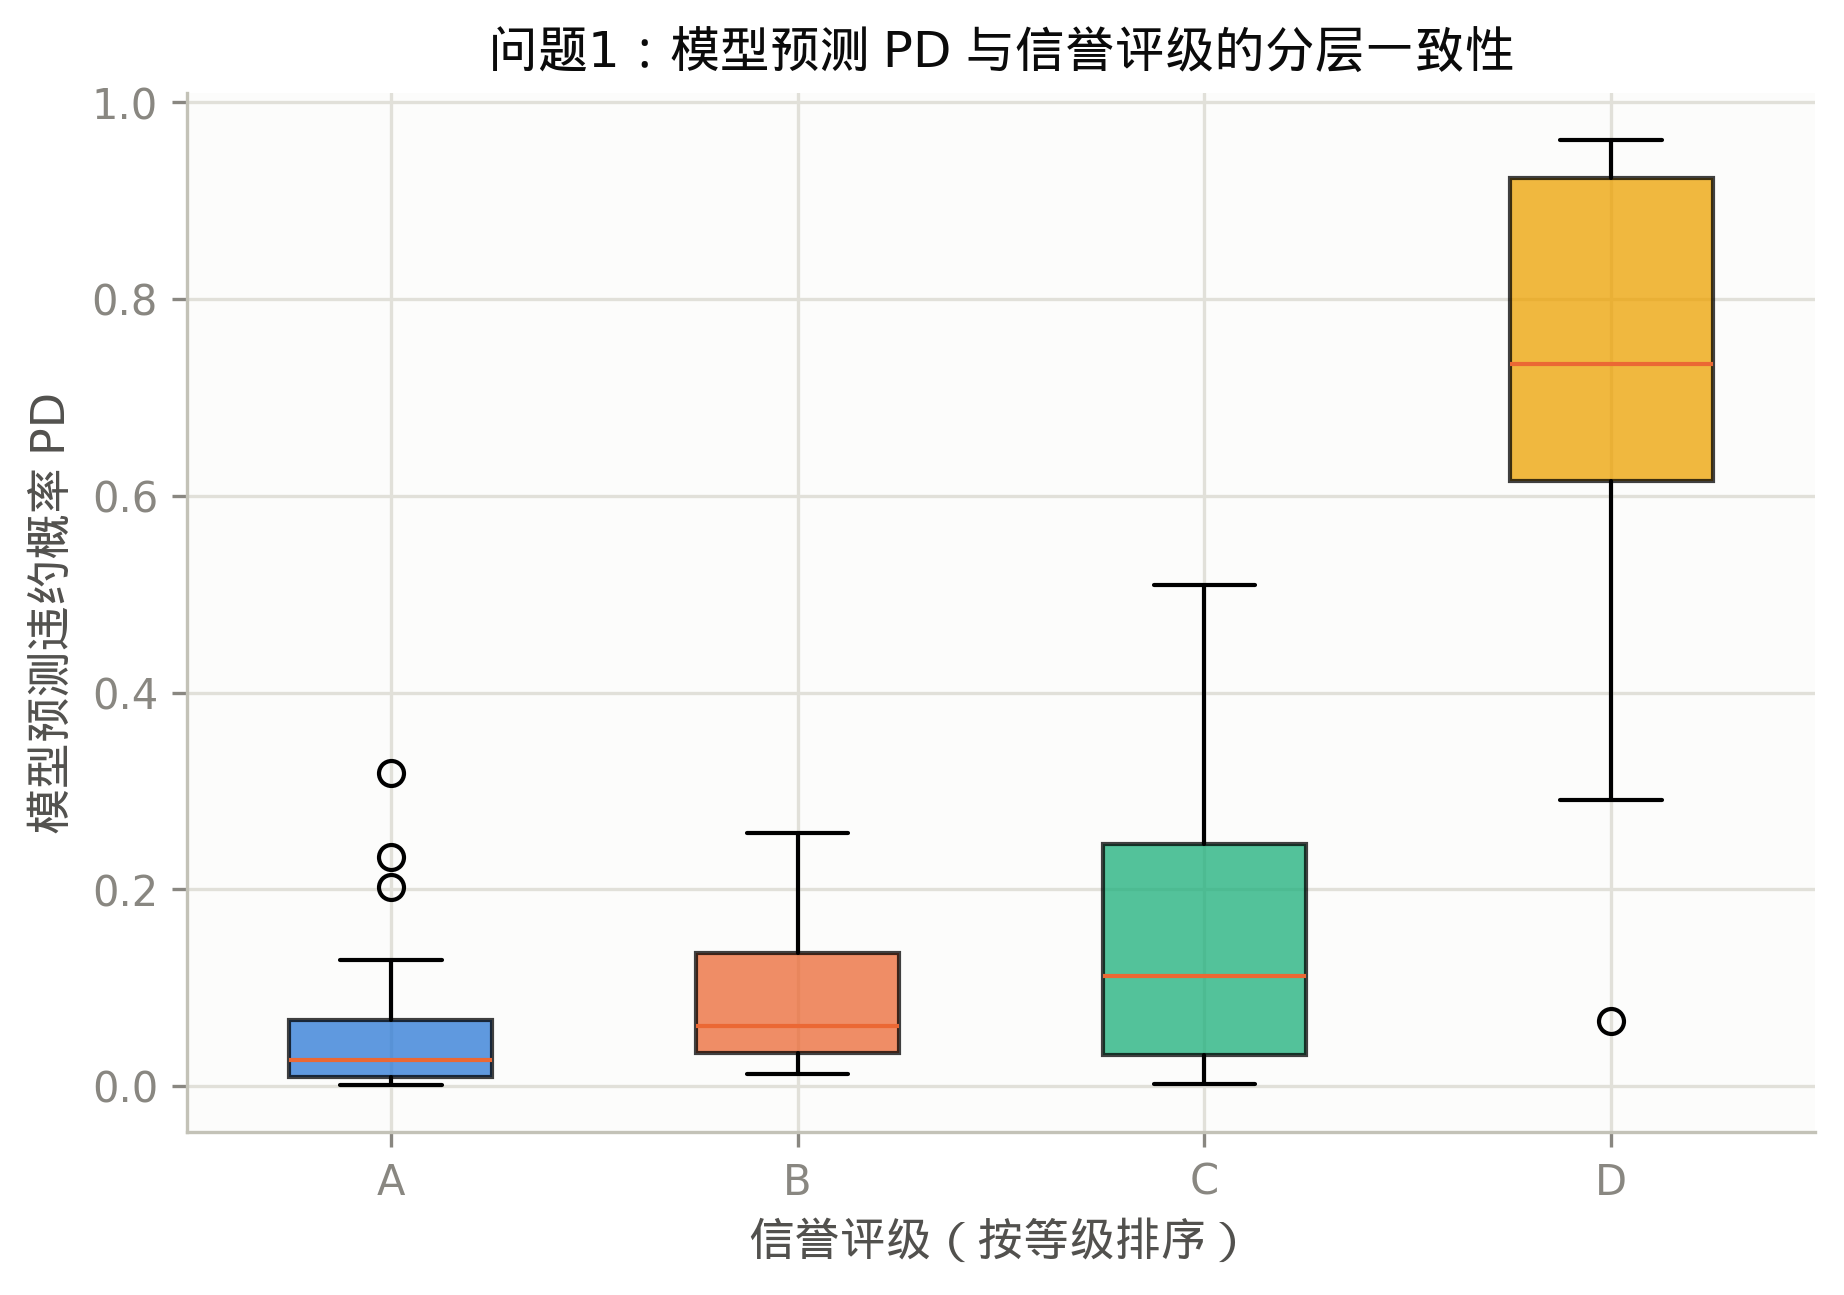
\includegraphics[width=\textwidth]{images/fig10_02_pd_by_rating.png}
        \caption{预测PD按评级分布}
        \label{fig:pd_by_rating}
    \end{minipage}
\end{figure}

\begin{figure}[H]
    \centering
    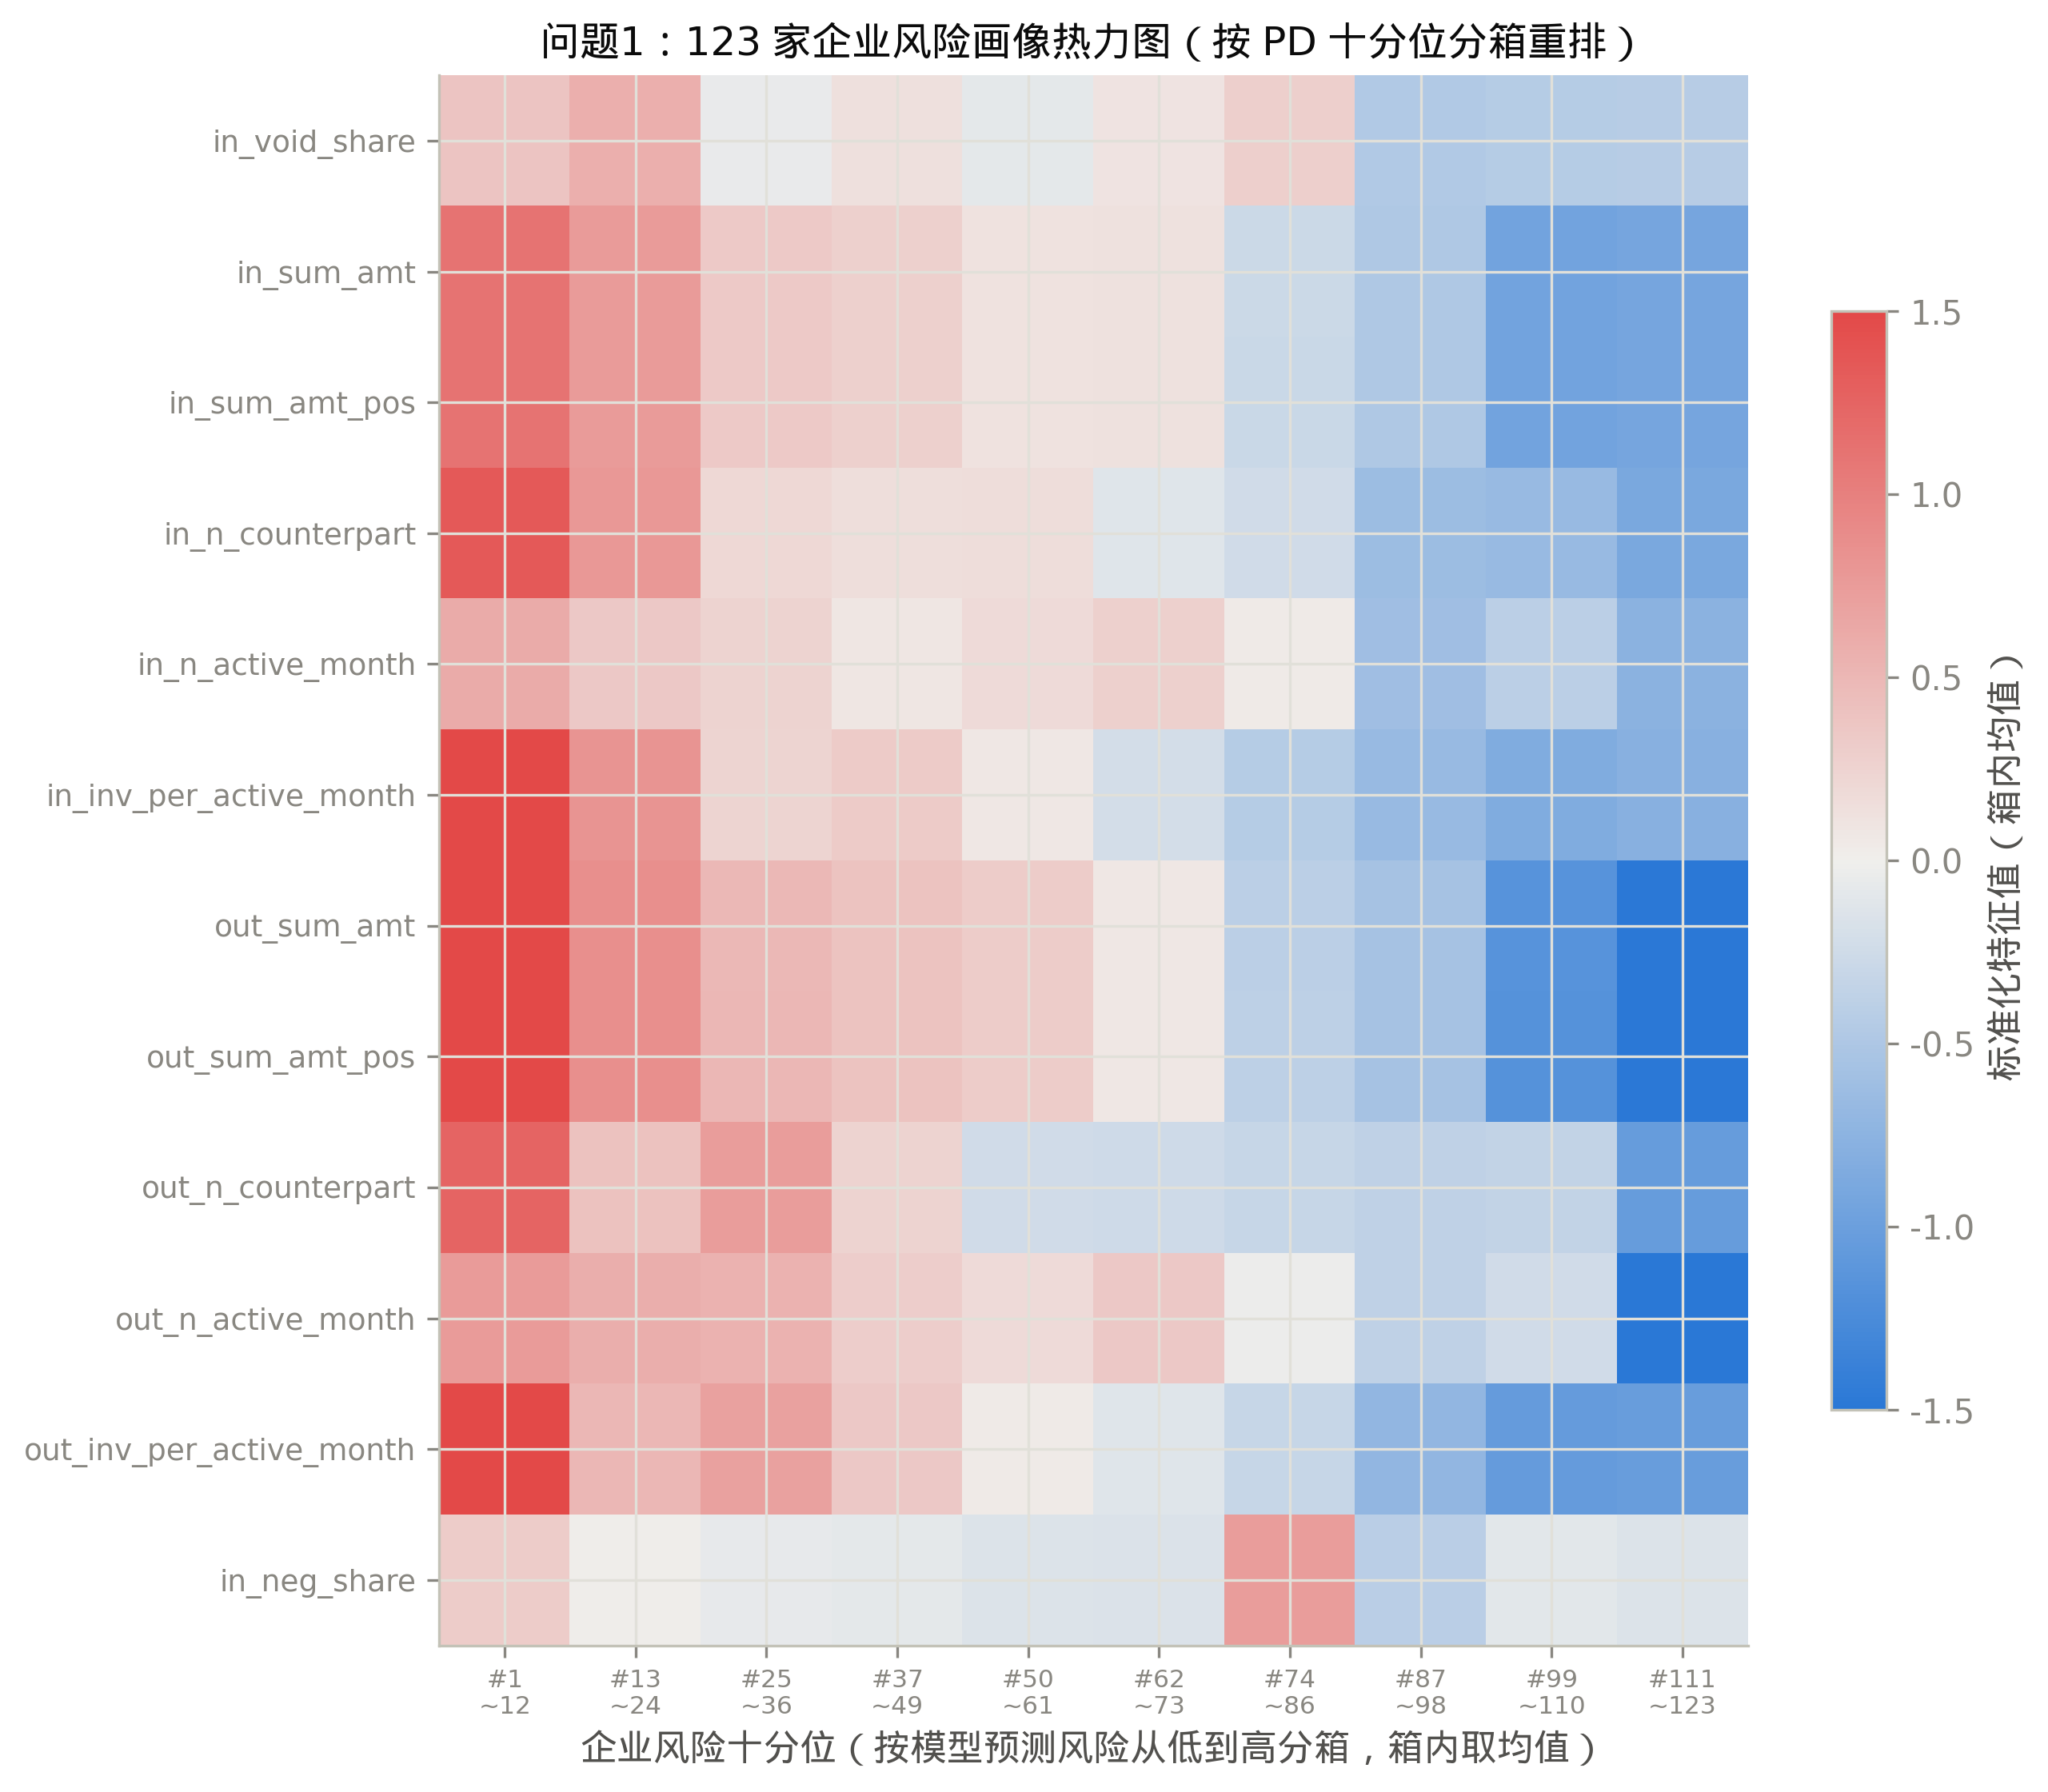
\includegraphics[width=0.62\textwidth]{images/fig10_03_risk_heatmap.png}
    \caption{123家企业风险画像热力图（按PD十分位分箱、箱内取均值，信用风险可视化惯例\cite{Dickson2011}）}
    \label{fig:risk_heatmap}
\end{figure}

\subsubsection{信贷策略：利率-流失率权衡与期望收益最大化分配}

设企业$i$的评级/层级为$k(i)$，在利率$r$下，单位额度的期望收益为：

\begin{equation}
    \pi_i(r) = \left[1 - c_{k(i)}(r)\right] \cdot \left[ r\left(1-\mathrm{PD}_i\right) - \mathrm{PD}_i\left(1-R\right)\right],
    \label{eq:profit_unit}
\end{equation}

其中第一项为"客户接受贷款"的概率（流失率的互补），第二项为毛期望收益（利息收入扣除期望违约损失，$R$为回收率，基准取0）。附件3的利率-流失率曲线（图~\ref{fig:churn}）显示流失率随利率单调上升，故存在使$\pi_i$最大的内部最优利率。在利率网格$r\in\{4.0\%,4.25\%,4.65\%,\dots,15\%\}$上搜索得到每家企业的最优利率$r_i^*$与单位期望收益$\pi_i^*=\pi_i(r_i^*)$；$\pi_i^*\le0$的企业不予放贷。最优利率随PD上升而上升（图~\ref{fig:opt_rate}），低风险企业获得低利率优惠，与题意"对信誉高、信贷风险小的企业给予利率优惠"一致。

\begin{figure}[H]
    \centering
    \begin{minipage}[t]{0.48\textwidth}
        \centering
        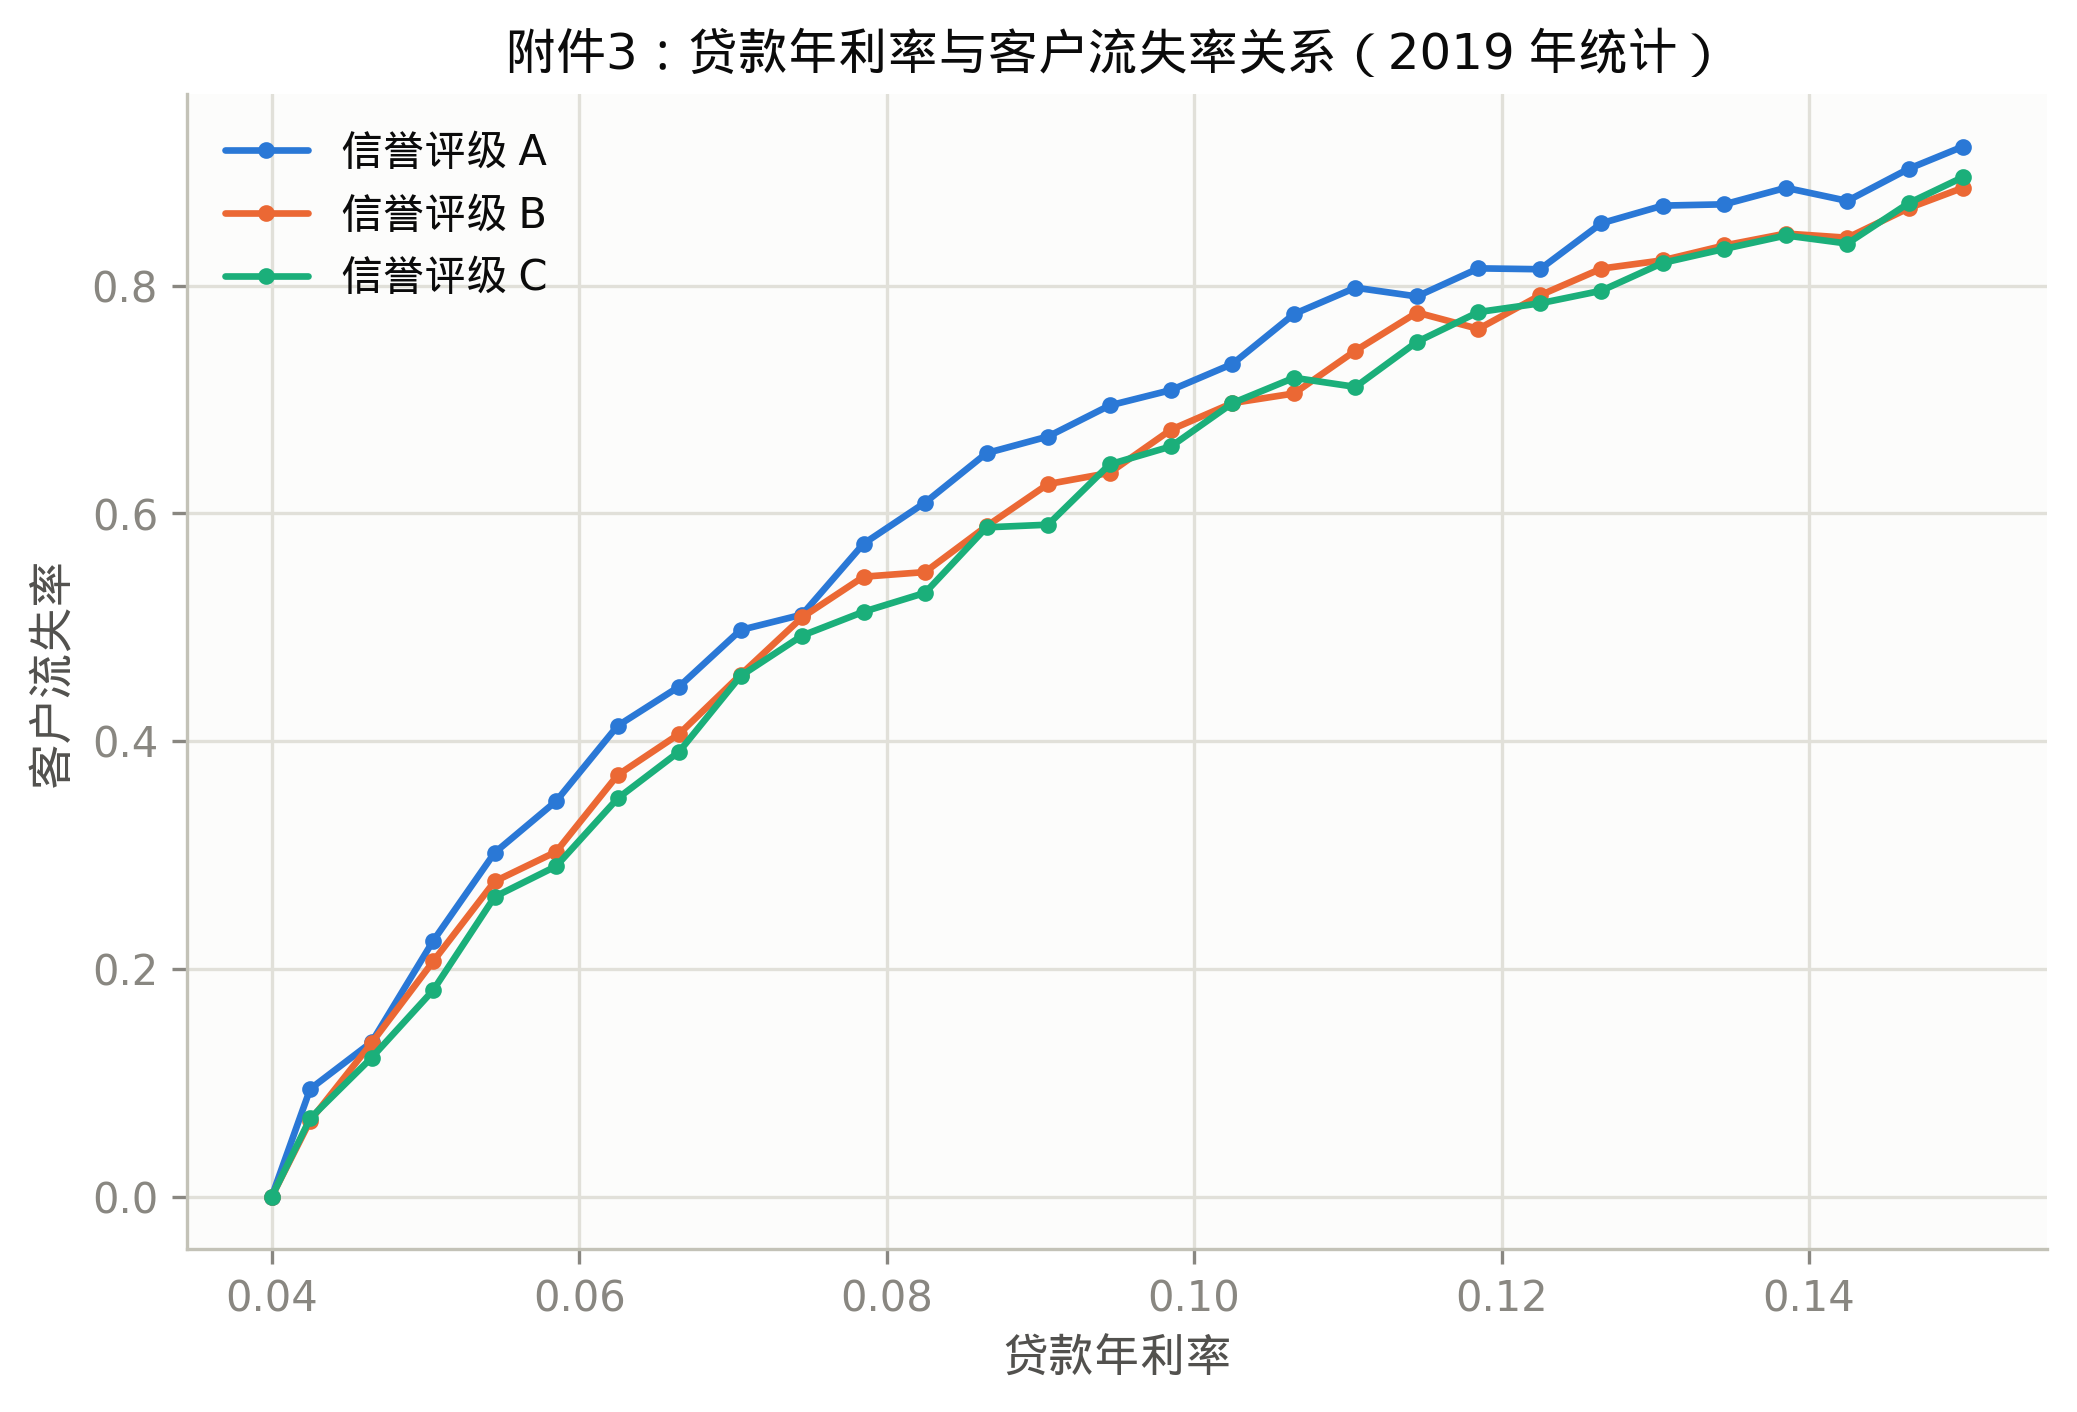
\includegraphics[width=\textwidth]{images/fig00_03_churn_rate_curves.png}
        \caption{附件3利率-流失率曲线}
        \label{fig:churn}
    \end{minipage}
    \hfill
    \begin{minipage}[t]{0.48\textwidth}
        \centering
        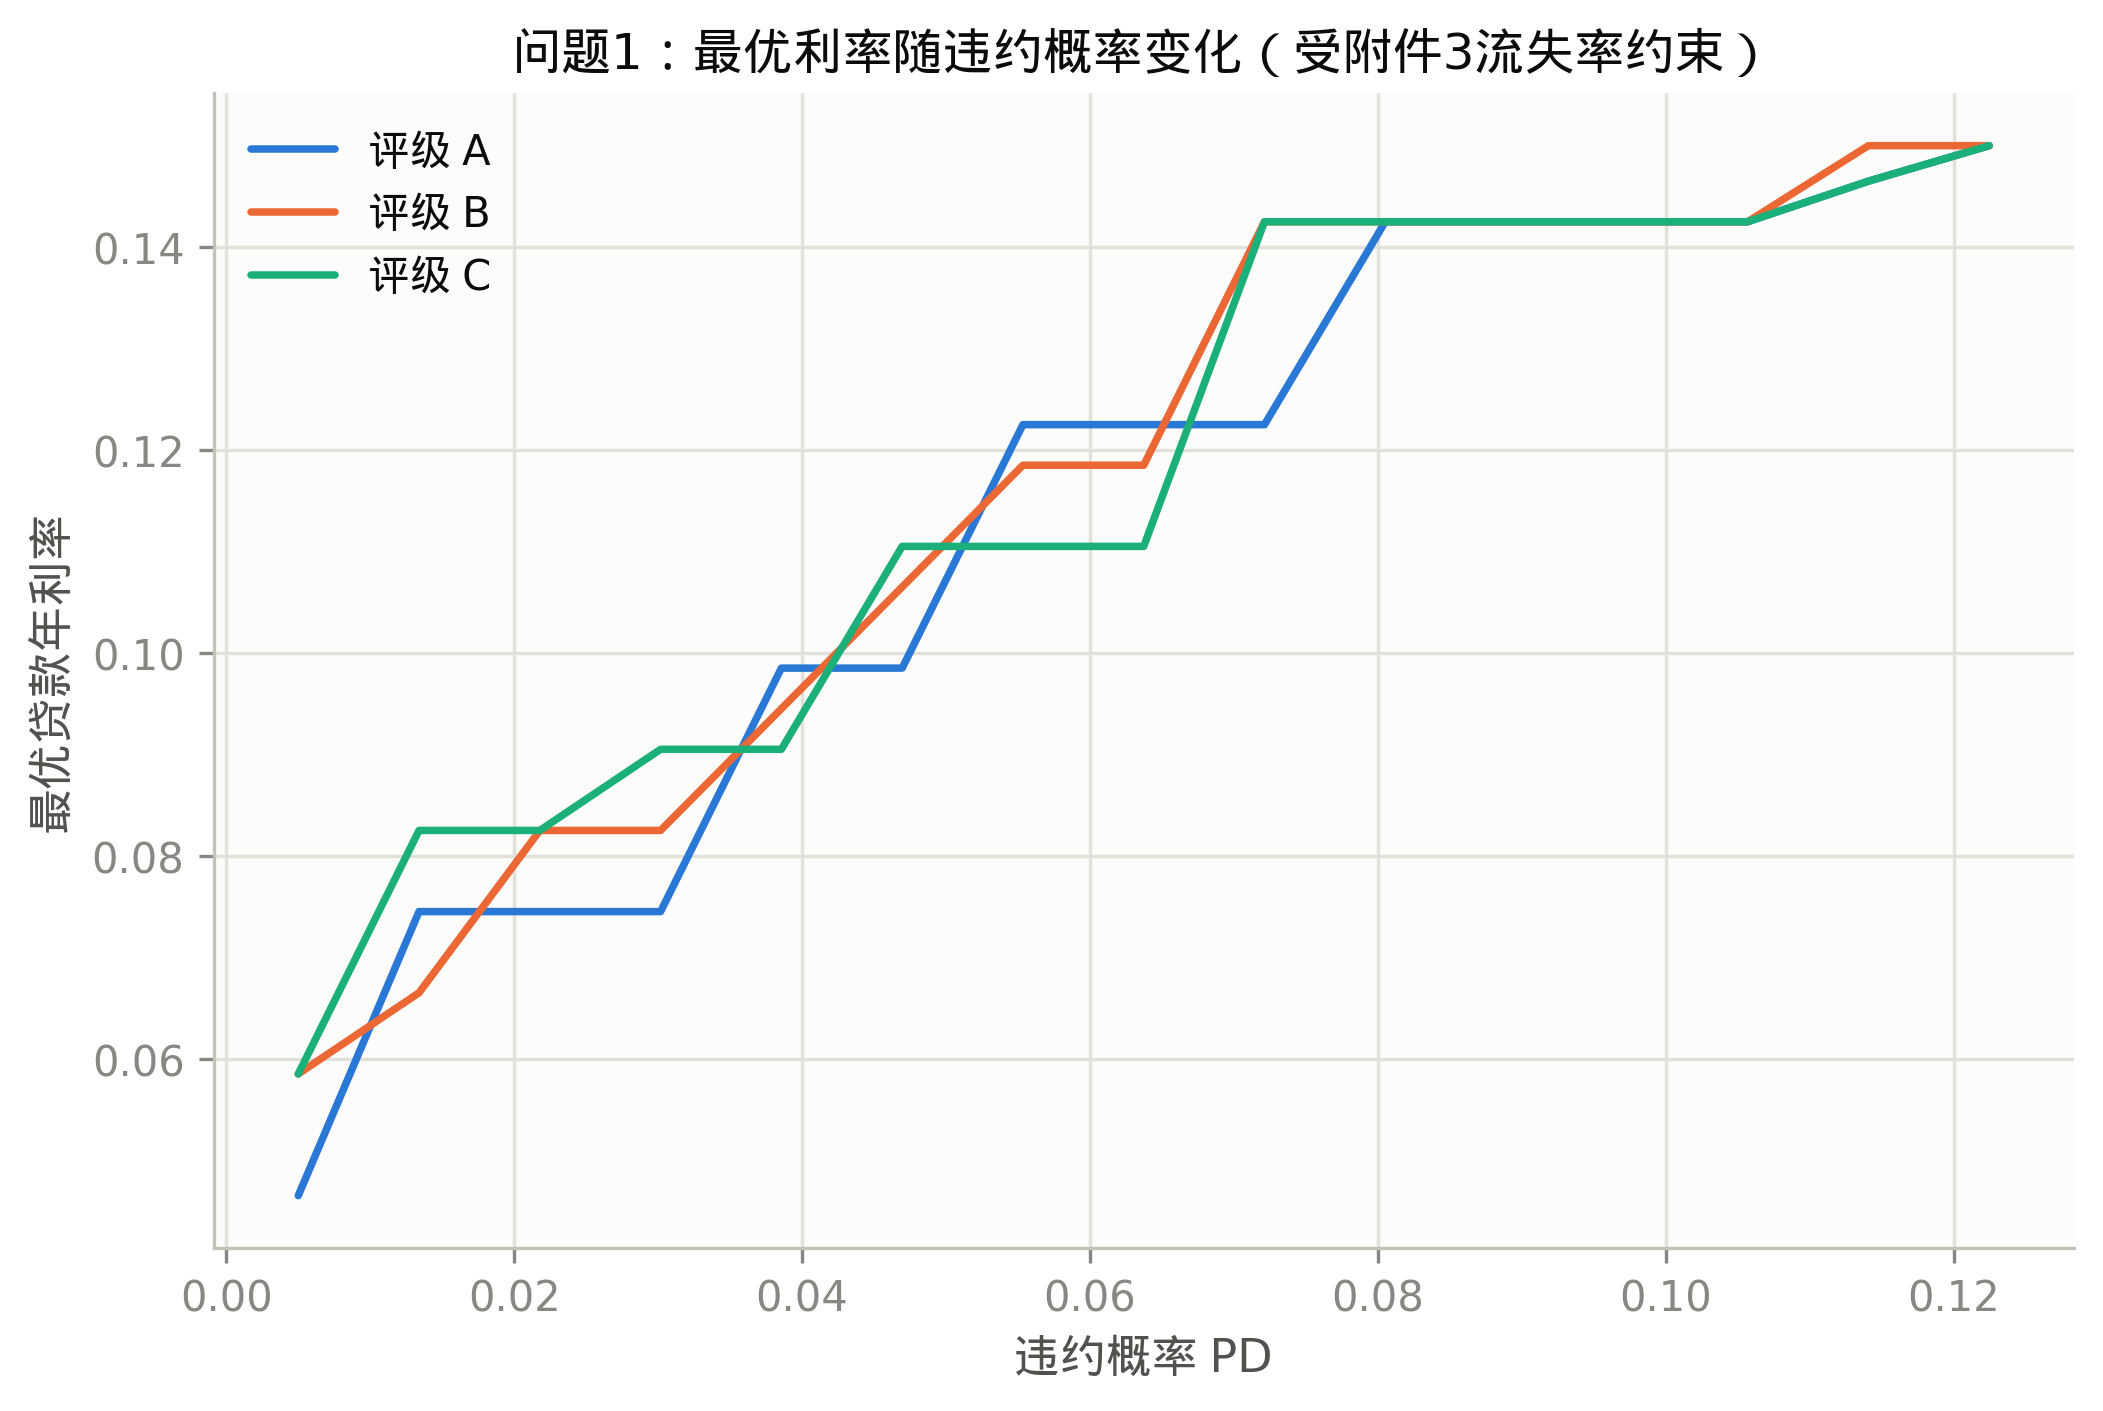
\includegraphics[width=\textwidth]{images/fig10_04_optimal_rate.png}
        \caption{最优利率随违约概率变化}
        \label{fig:opt_rate}
    \end{minipage}
\end{figure}

企业$i$的额度上限取评级上限与年销项额比例的较小者：

\begin{equation}
    \text{cap}_i = \min\left\{C_{k(i)},\ \theta S_i\right\}, \qquad
    C_A=1000,\ C_B=500,\ C_C=300,\ C_D=0\ \text{（万元）},\ \theta=0.25.
    \label{eq:cap}
\end{equation}

评级D企业不予放贷（与题意一致）。在年度信贷总额$T$固定时，策略为求解：

\begin{equation}
    \max_{\{A_i\}}\ \sum_{i} A_i\,\pi_i^* \qquad
    \text{s.t.}\quad \sum_i A_i \le T,\quad 0\le A_i\le \text{cap}_i,\quad A_i\in\mathbb{Z}_+,
    \label{eq:alloc}
\end{equation}

目标函数对$A_i$线性，属于线性背包问题，按单位期望收益$\pi_i^*$降序依次填满额度上限即为最优（贪心法）。这一"期望收益框架下借贷组合分配"的思路与文献\cite{Byanjankar2021}一致。图~\ref{fig:alloc_p1}给出总额1亿元时的分配结构：放贷14家（A级10家、B级2家、C级2家），实际分配恰好1亿元，期望收益352万元。表~\ref{tab:coverage}给出覆盖曲线：随总额从2000万元增至5亿元，放贷家数从3家增至71家、期望收益从78万元增至834万元；总额超过约3.7亿元后触及企业额度上限总和，出现分配饱和。

\begin{table}[H]
\centering
\caption{问题一：总额-覆盖曲线}
\label{tab:coverage}
\begin{tabular}{ccccccc}
\toprule
总额（万元） & 2000 & 5000 & 10000 & 15000 & 20000 & 30000 \\
\midrule
放贷家数 & 3 & 7 & 14 & 21 & 31 & 54 \\
期望收益（万元） & 78 & 190 & 352 & 496 & 616 & 790 \\
\bottomrule
\end{tabular}
\end{table}

覆盖曲线揭示了该策略的经济学特征：期望收益随总额增加呈现\textbf{边际递减}——总额从2000万元增至1亿元时收益增加274万元（每1000万元新增约34万元），而从1亿元增至3亿元时仅增加438万元（每1000万元新增约22万元）。原因是额度分配按单位期望收益降序进行，预算扩张只能惠及边际收益更低的企业；当总额超过约3.7亿元（所有可贷企业额度上限之和）时分配饱和，说明该银行对这批企业的信贷容量存在自然上限。这一曲线可直接作为银行"总额—收益"预算决策的依据。

\begin{figure}[H]
    \centering
    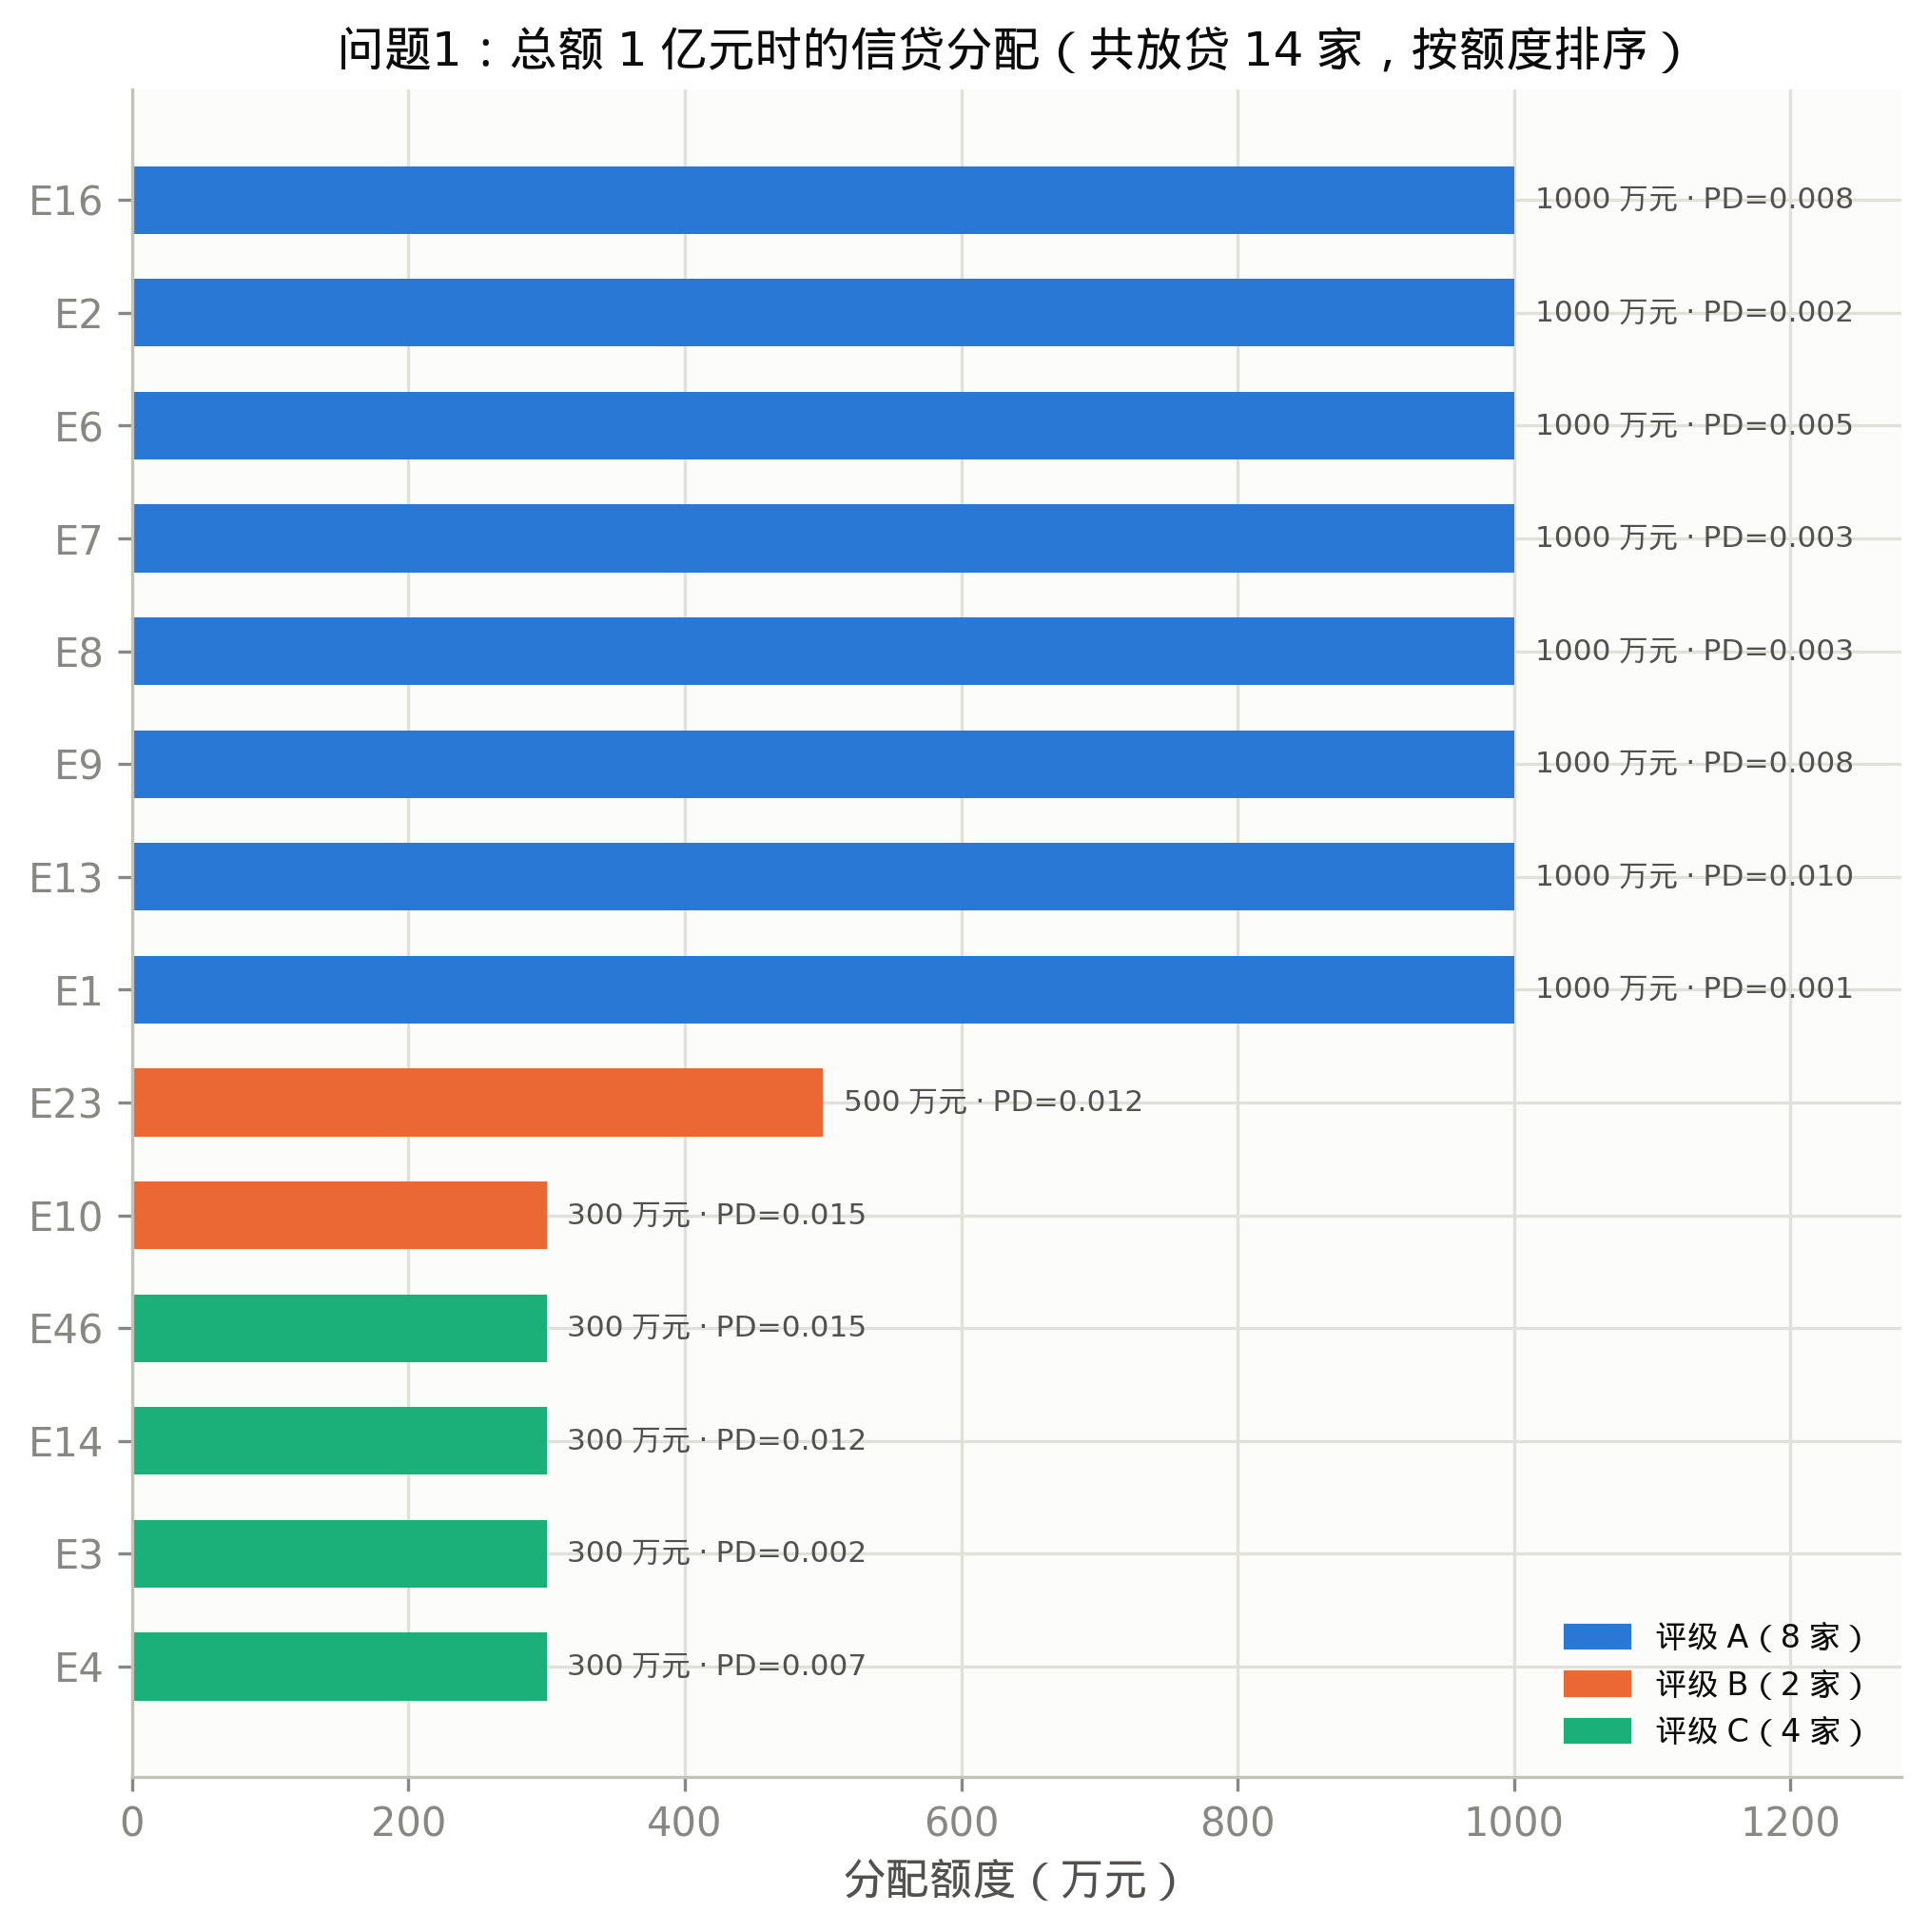
\includegraphics[width=0.78\textwidth]{images/fig10_05_allocation_by_rating.png}
    \caption{问题一：1亿元信贷分配明细（14家放贷企业按额度排序，条形右侧标注实际额度与PD）}
    \label{fig:alloc_p1}
\end{figure}

表~\ref{tab:p1_detail}~给出总额1亿元时放贷企业的额度与利率明细：8家A级企业各获1000万元上限额度、利率4.65\%--5.85\%，2家B级企业各获300--500万元、利率5.85\%--6.65\%，体现出"低风险低利率、大额度"的差异化定价。

\begin{table}[H]
\centering
\caption{问题一：总额1亿元时的放贷明细（按额度降序，前10家）}
\label{tab:p1_detail}
{\small
\begin{tabular}{cccccc}
\toprule
\textbf{企业} & \textbf{评级} & \textbf{PD} & \textbf{利率} & \textbf{额度(万元)} & \textbf{期望收益(万元)} \\
\midrule
E1  & A & 0.0011 & 4.65\% & 1000 & 39.16 \\
E2  & A & 0.0021 & 4.65\% & 1000 & 38.30 \\
E8  & A & 0.0025 & 4.65\% & 1000 & 37.89 \\
E7  & A & 0.0031 & 4.65\% & 1000 & 37.34 \\
E6  & A & 0.0055 & 4.65\% & 1000 & 35.25 \\
E16 & A & 0.0077 & 4.65\% & 1000 & 33.21 \\
E9  & A & 0.0078 & 4.65\% & 1000 & 33.13 \\
E13 & A & 0.0105 & 5.85\% & 1000 & 30.93 \\
E23 & B & 0.0122 & 5.85\% & 500  & 15.89 \\
E10 & B & 0.0151 & 6.65\% & 300  & 8.98 \\
\bottomrule
\end{tabular}}
\end{table}

\subsection{问题二：附件2风险量化迁移与1亿元信贷策略}

\subsubsection{迁移打分与分布偏移检验}

问题一的评分器（逻辑回归+标准化器+特征清单）仅依赖发票特征，直接应用于附件2的302家企业，得到迁移违约概率PD（均值0.188、最大0.988）。迁移有效性以PSI（群体稳定性指数）检验两样本特征分布偏移：

\begin{equation}
    \text{PSI} = \sum_{j=1}^{10} \left(\hat{p}_j^{\text{A2}} - \hat{p}_j^{\text{A1}}\right)
    \ln\frac{\hat{p}_j^{\text{A2}}}{\hat{p}_j^{\text{A1}}},
    \label{eq:psi}
\end{equation}

其中$\hat{p}_j$为第$j$个分位箱的占比。如图~\ref{fig:psi}~所示，销项额与进项额的PSI约0.22--0.24（轻度偏移），作废率PSI 0.19，而对手方数、活跃度、进销比等结构特征PSI均小于0.1（稳定），说明附件2企业整体规模偏小但经营结构类似，迁移打分合理。图~\ref{fig:dist_a1a2}直观对比两样本关键特征分布。

\begin{figure}[H]
    \centering
    \begin{minipage}[t]{0.48\textwidth}
        \centering
        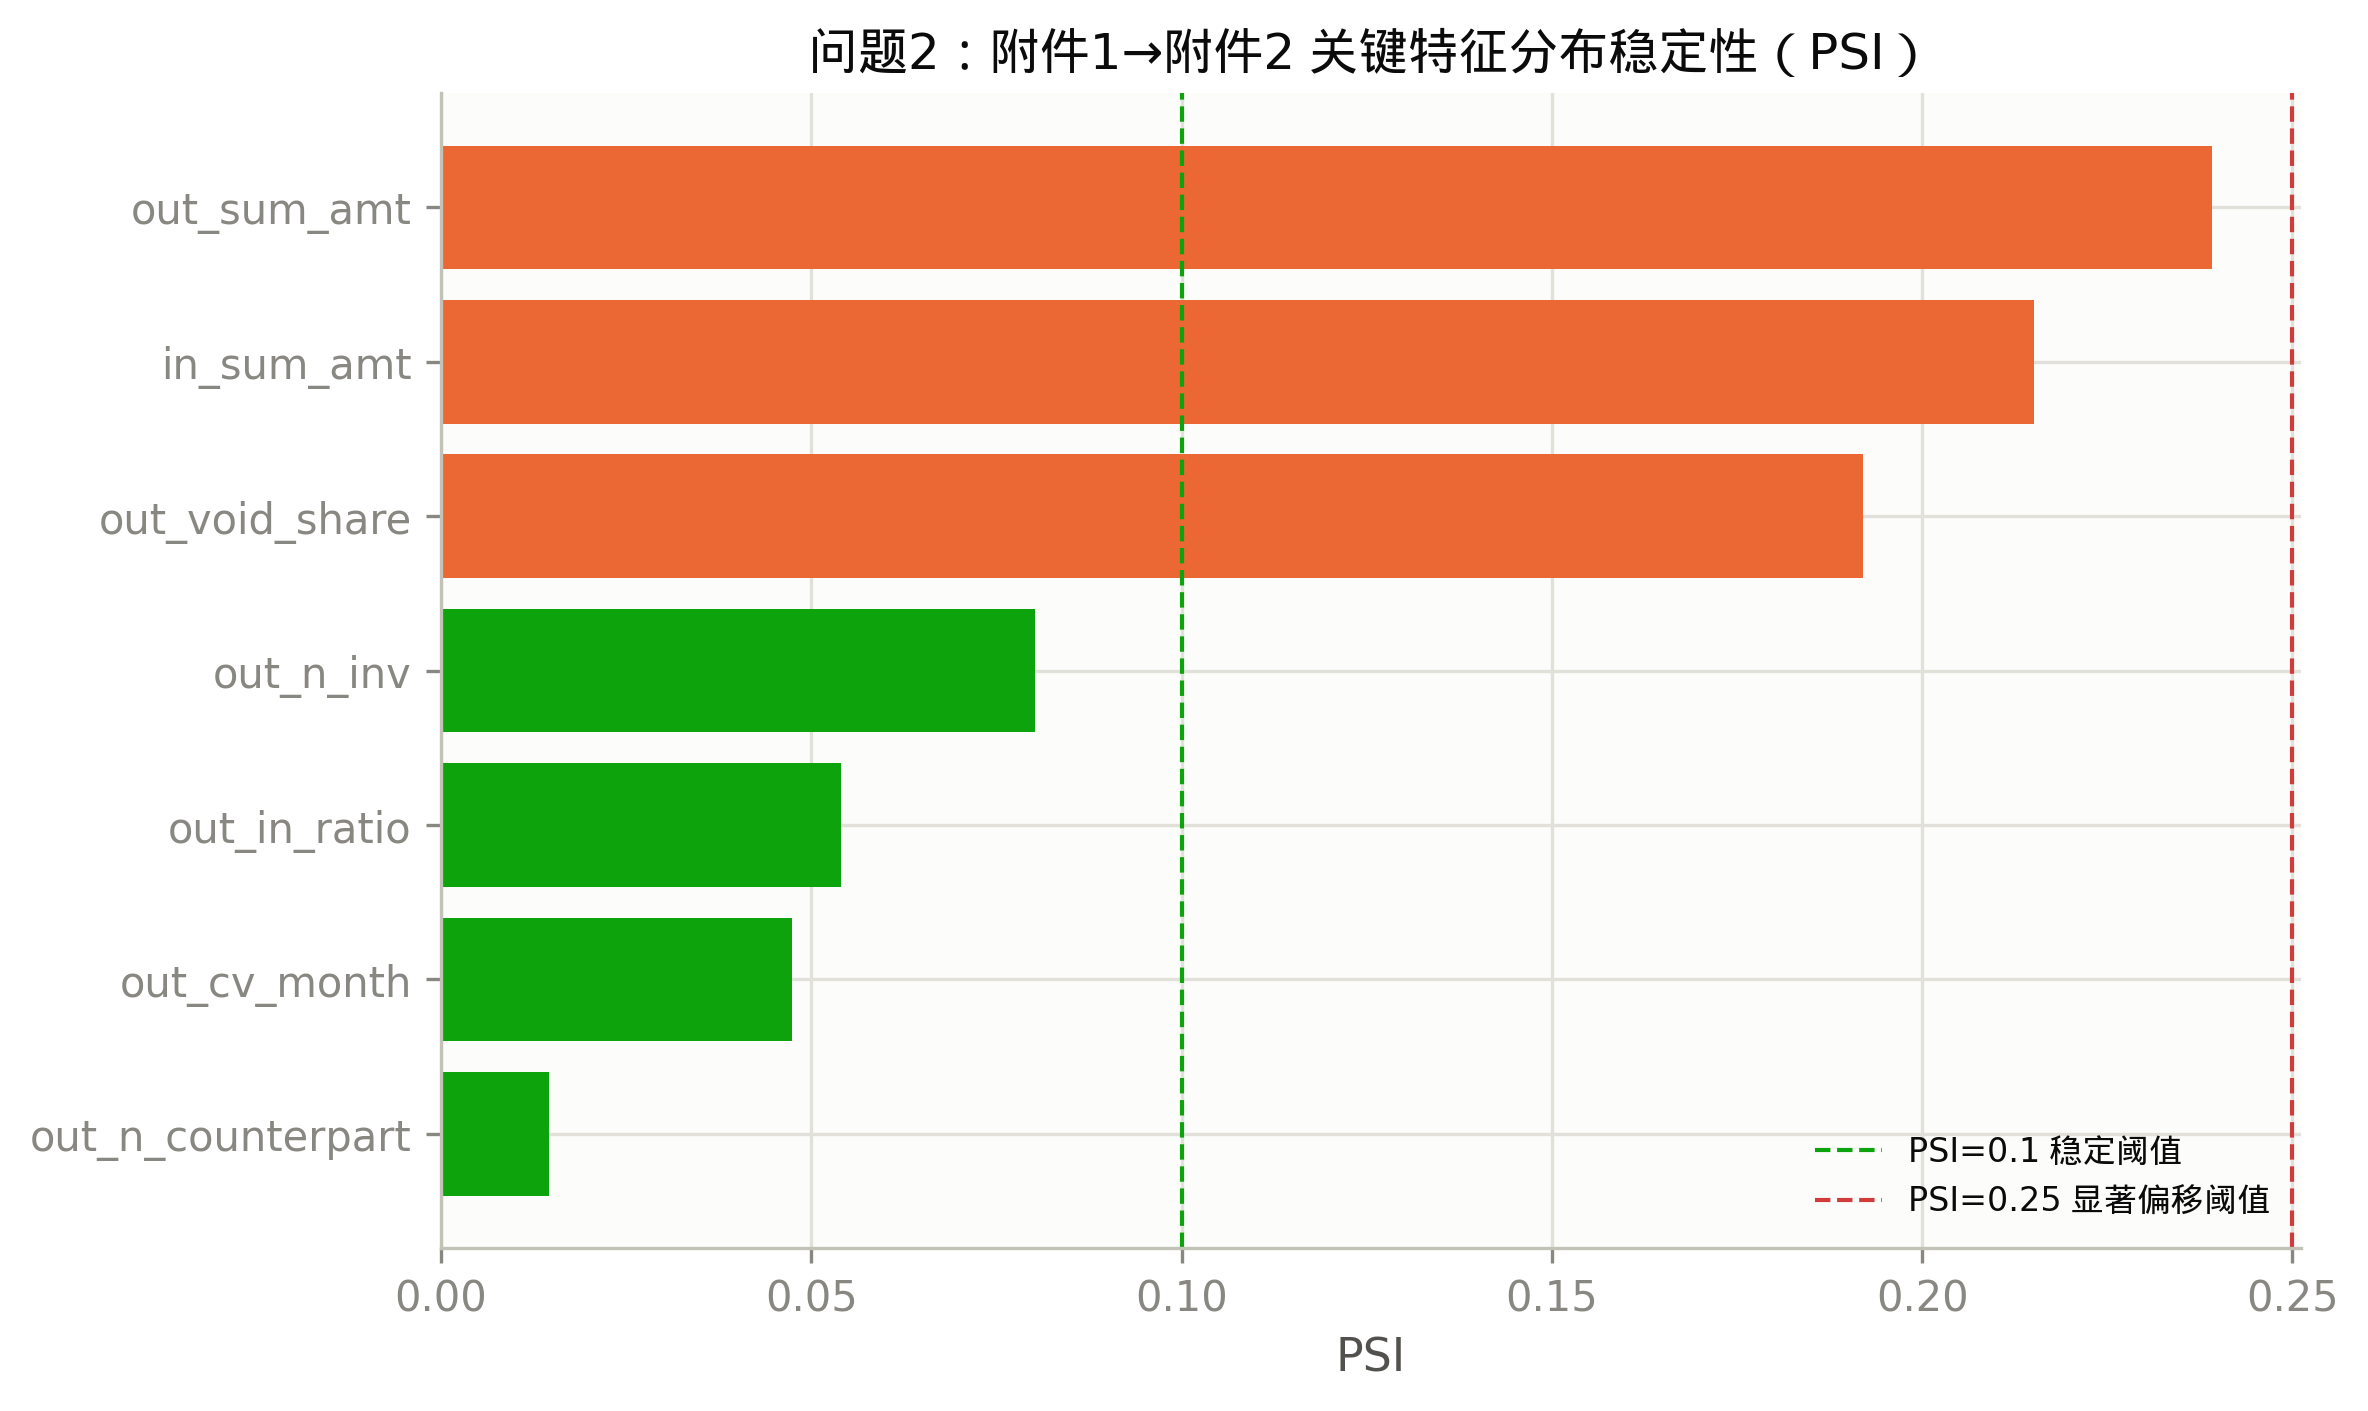
\includegraphics[width=\textwidth]{images/fig20_02_psi.png}
        \caption{特征分布偏移PSI（按PSI排序）}
        \label{fig:psi}
    \end{minipage}
    \hfill
    \begin{minipage}[t]{0.48\textwidth}
        \centering
        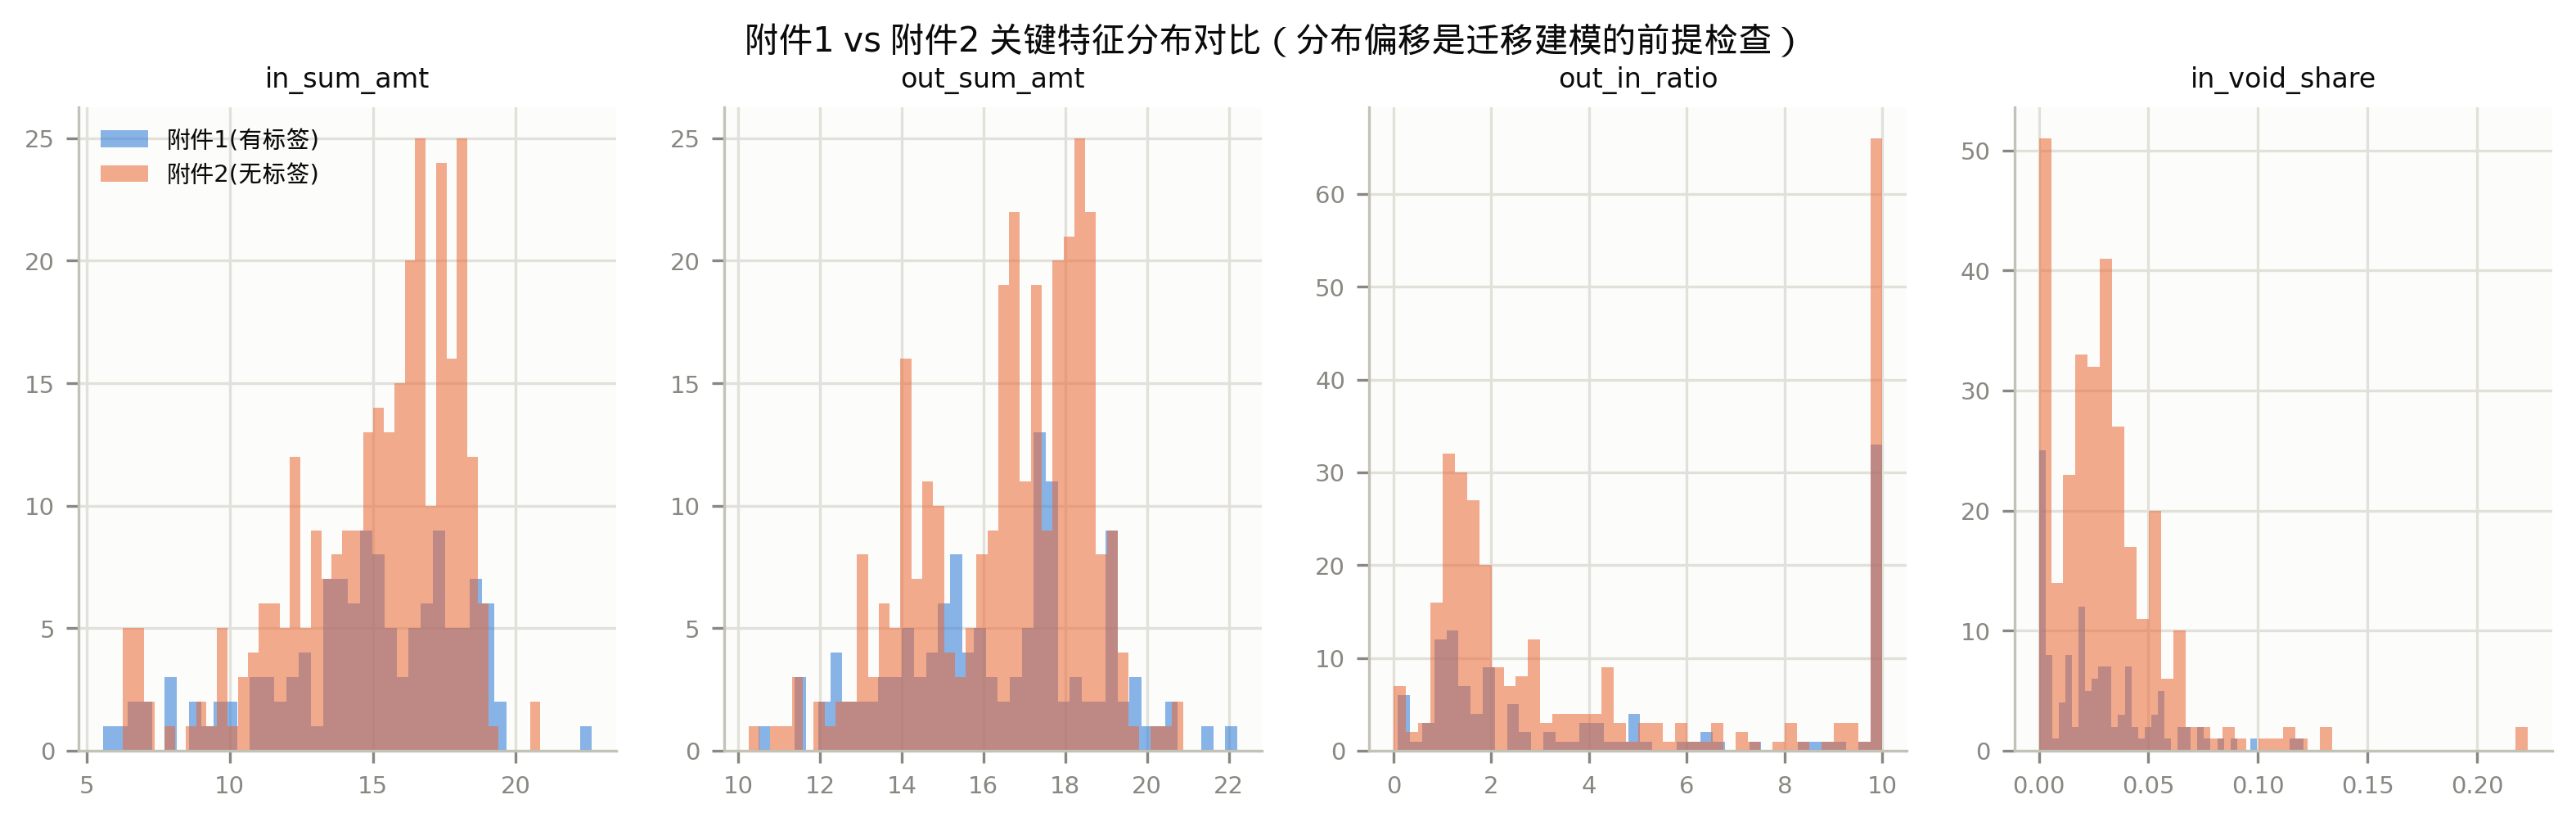
\includegraphics[width=\textwidth]{images/fig00_05_feature_distributions.png}
        \caption{附件1与附件2关键特征分布对比}
        \label{fig:dist_a1a2}
    \end{minipage}
\end{figure}

\subsubsection{伪评级分层}

附件2无信誉评级，无法直接套用附件3的分档流失率曲线。以问题一各评级PD均值（A=0.057、B=0.088、C=0.149、D=0.711）的相邻中点为阈值，将302家企业映射为伪评级：PD$<0.0723$为A、$<0.1185$为B、$<0.4299$为C、其余为D，得到A/B/C/D分别141/38/81/42家，层内PD均值0.031/0.098/0.234/0.705严格单调（图~\ref{fig:pd_hist}）。伪评级在问题二中承担三重角色：决定适用的流失率曲线、决定额度上限$C_k$、决定D层不予放贷的政策约束。

\begin{figure}[H]
    \centering
    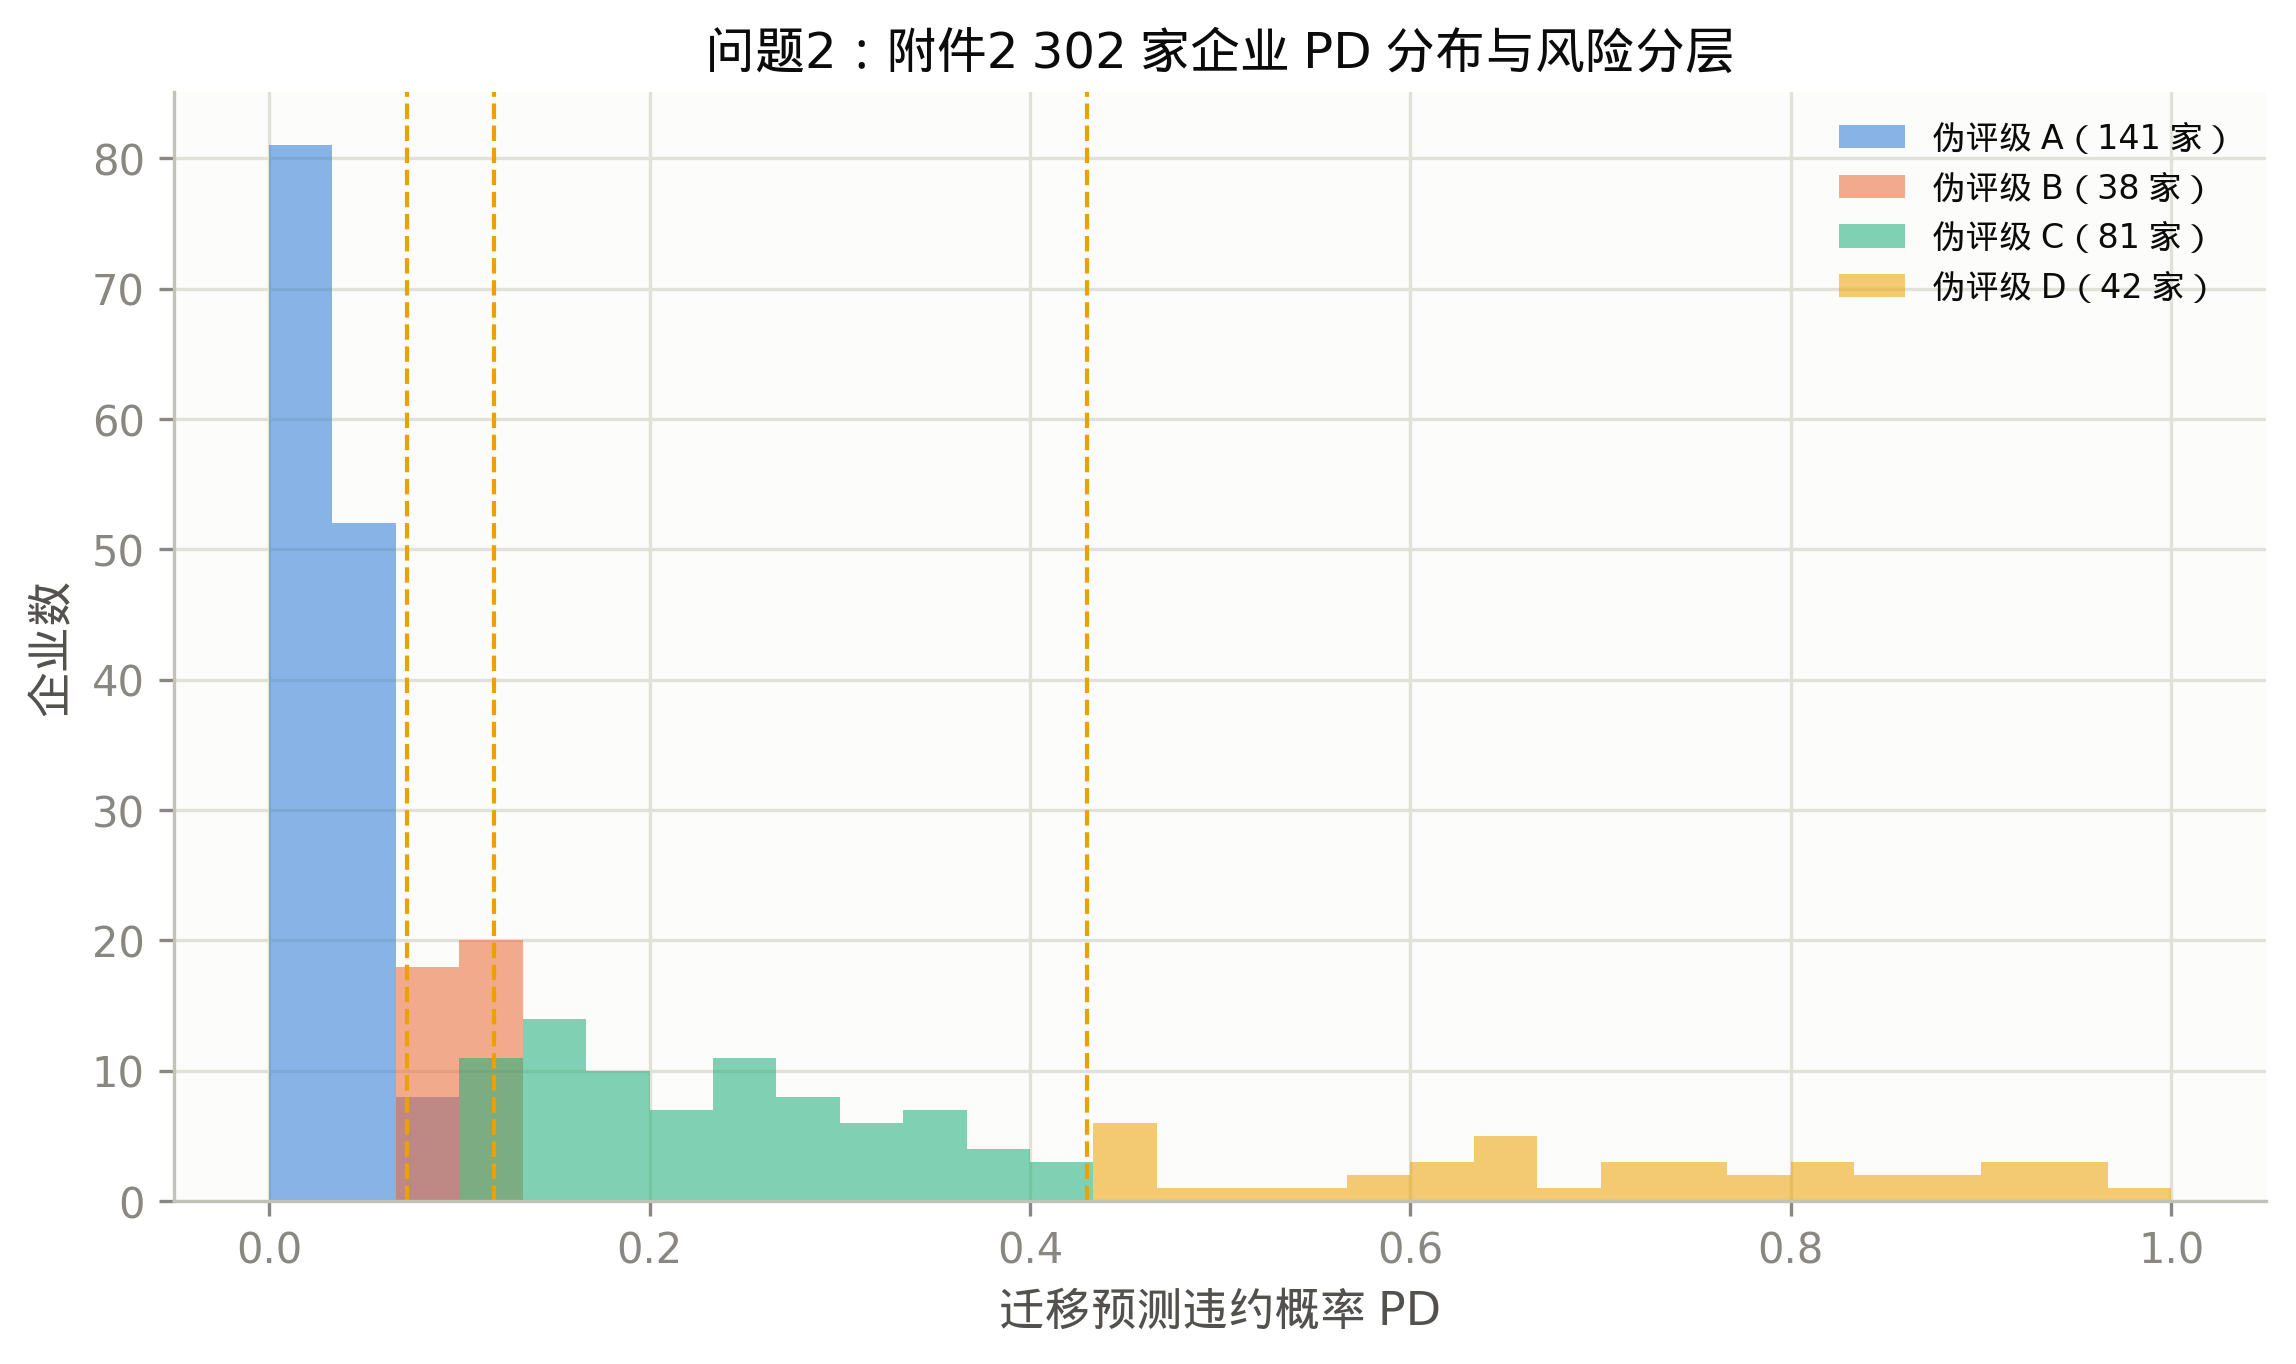
\includegraphics[width=0.72\textwidth]{images/fig20_01_pd_histogram.png}
    \caption{附件2迁移PD分布与伪评级分层}
    \label{fig:pd_hist}
\end{figure}

\subsubsection{1亿元信贷策略}

将式\eqref{eq:profit_unit}--\eqref{eq:alloc}的框架用于302家企业，总额$T=10000$万元，贪心分配结果如表~\ref{tab:p2_strategy}~所示：放贷12家（全部为伪评级A层），平均利率4.7\%，实际分配恰好1亿元，期望收益356万元。图~\ref{fig:alloc_p2}给出按风险层级排序的分配结构。与问题一（同预算14家）相比放贷家数接近，说明迁移打分与分层规则保持了策略的一致性。需要指出：在"评级上限×1000万元"的额度规则下，1亿元预算集中于约12--14家最优企业，覆盖-集中存在权衡（图~\ref{fig:profit_total}的覆盖曲线展示了预算扩张时的分散化进程）。

\begin{table}[H]
\centering
\caption{问题二：1亿元信贷策略汇总}
\label{tab:p2_strategy}
\begin{tabular}{cccc}
\toprule
\textbf{指标} & \textbf{数值} & \textbf{指标} & \textbf{数值} \\
\midrule
放贷家数 & 12（全部A层） & 平均利率 & 4.7\% \\
实际分配 & 10000万元 & 期望收益 & 356万元 \\
放贷企业平均PD & 0.005 & 未放贷 & 290家 \\
\bottomrule
\end{tabular}
\end{table}

\begin{figure}[H]
    \centering
    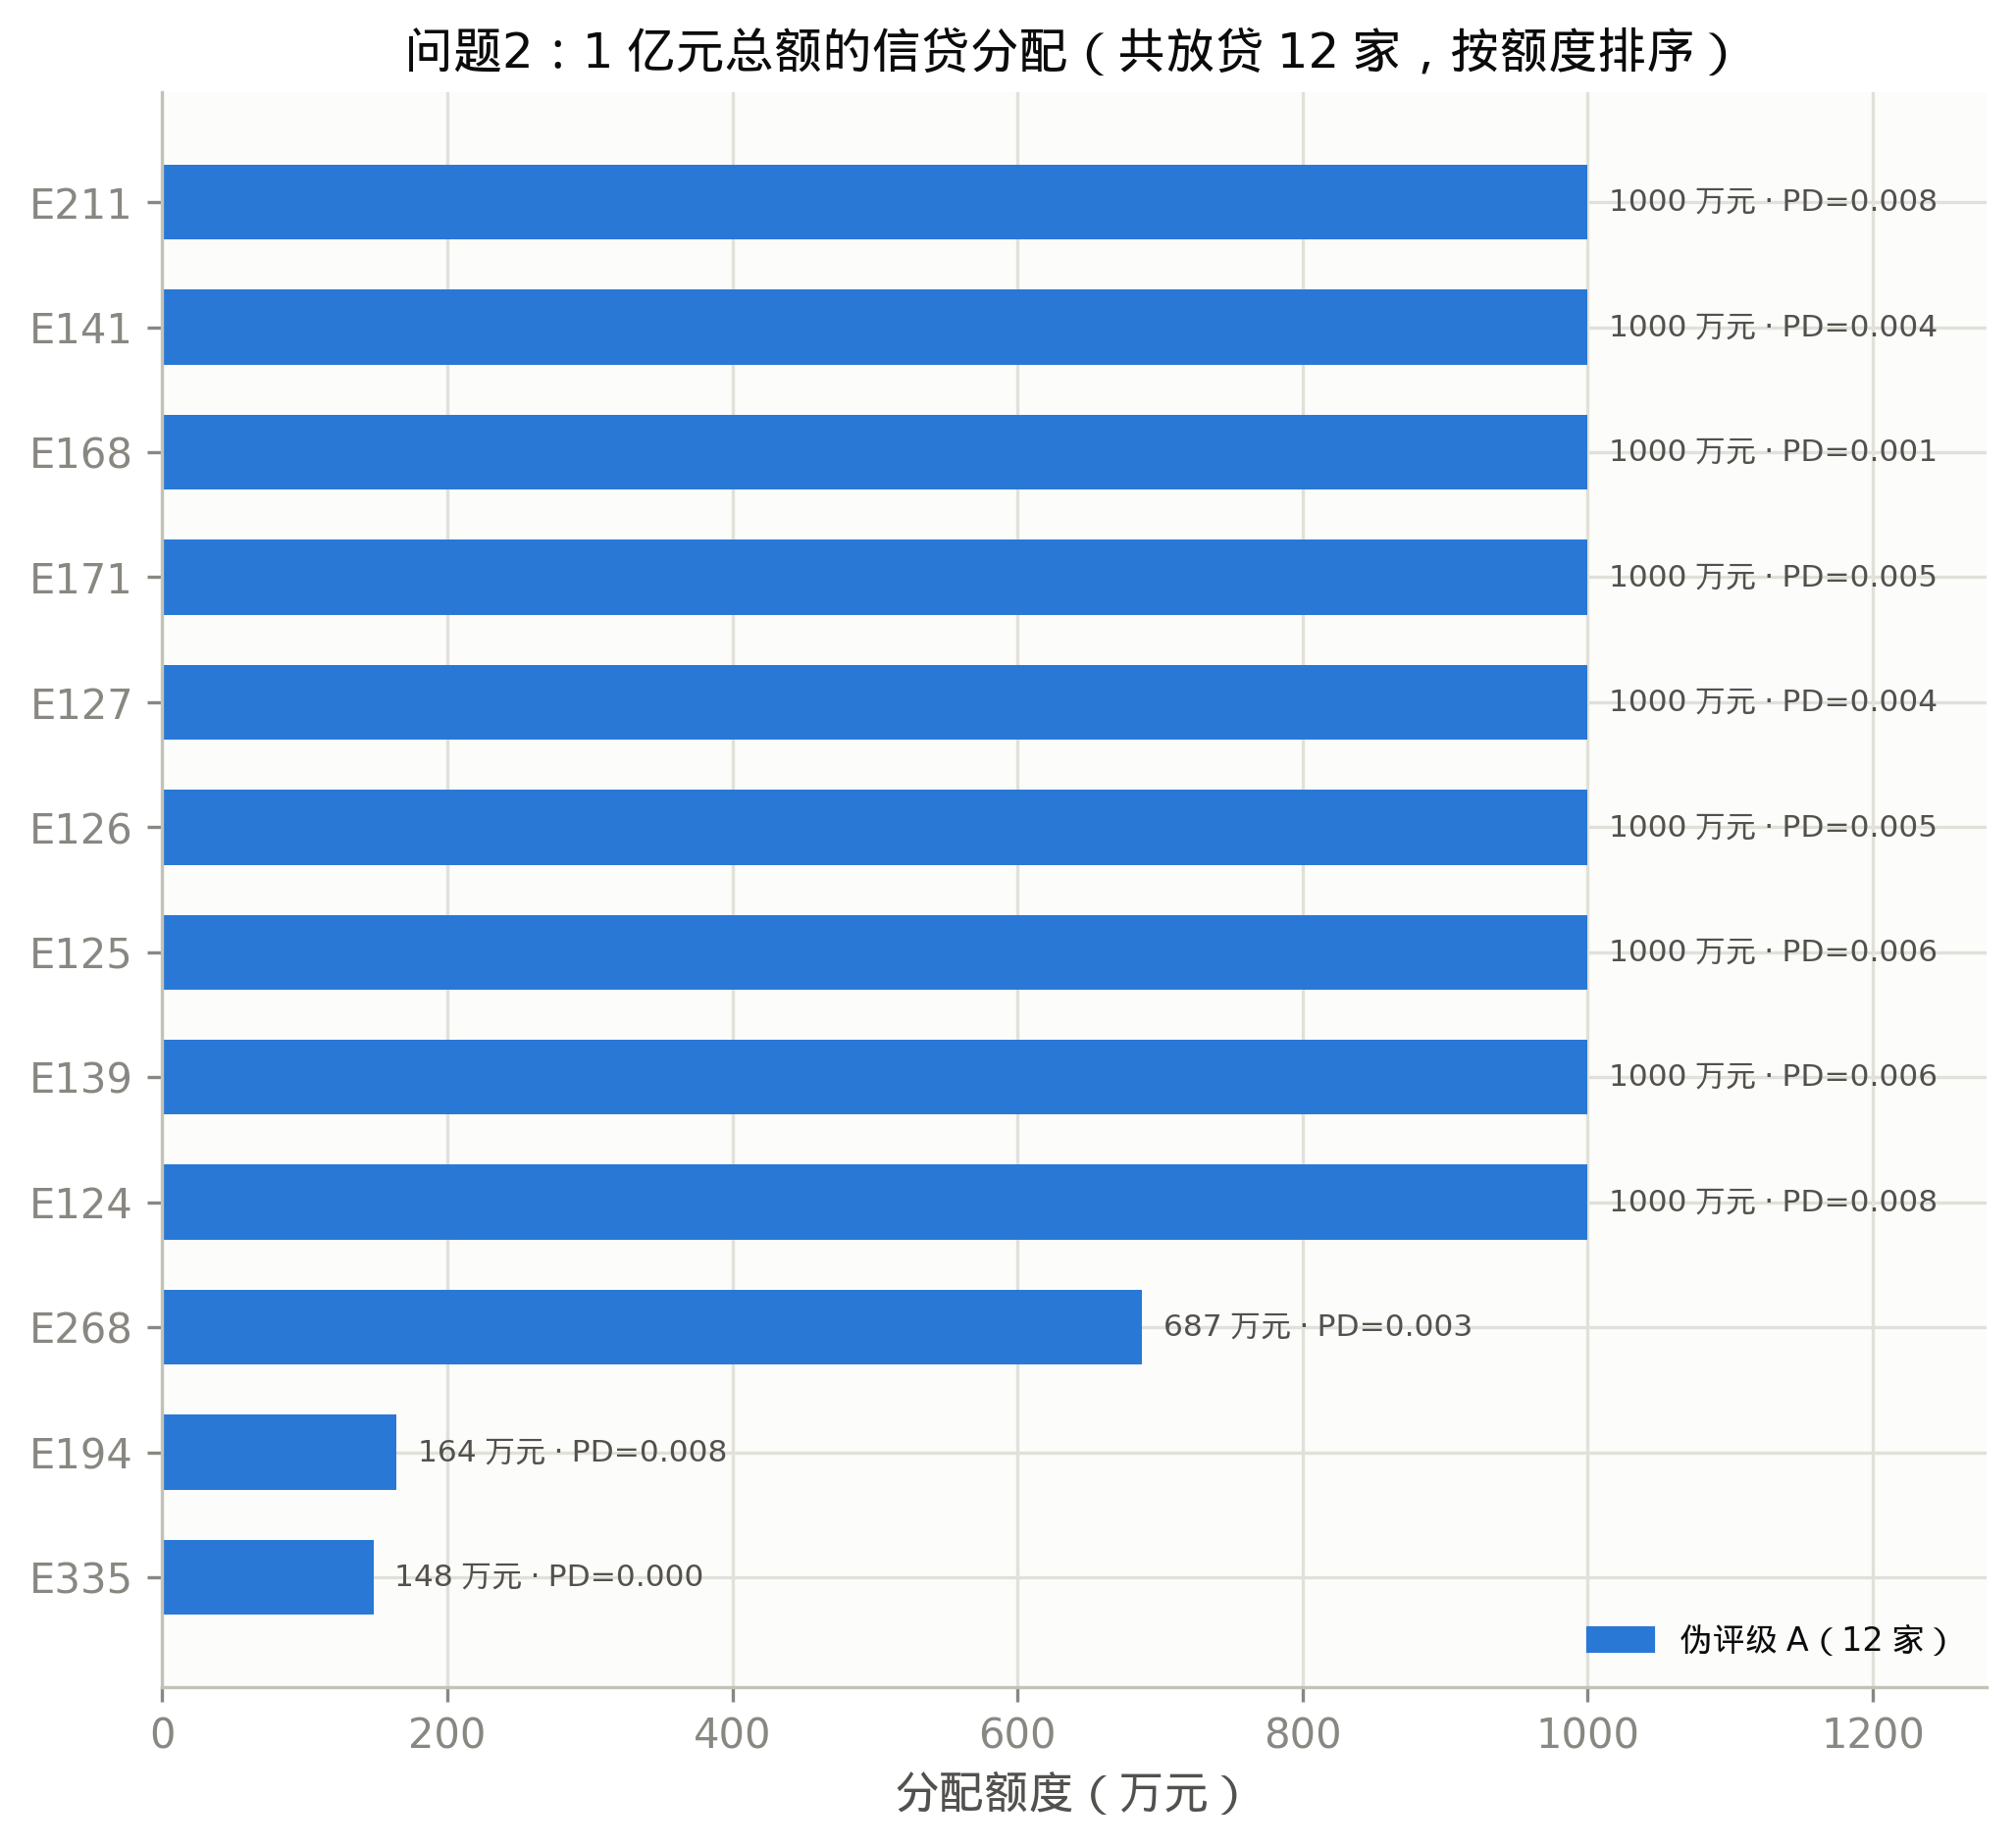
\includegraphics[width=0.78\textwidth]{images/fig20_03_allocation_by_tier.png}
    \caption{问题二：1亿元信贷分配明细（12家放贷企业按额度排序，条形右侧标注实际额度与PD）}
    \label{fig:alloc_p2}
\end{figure}

表~\ref{tab:p2_detail}~给出12家放贷企业的明细：均为伪评级A层，PD均低于0.01，额度除个别企业受25\%销项额约束外多为1000万元上限，利率统一为4.65\%的A层最优水平。290家未放贷企业中，D层42家因政策约束全部排除，B/C层企业因单位期望收益低于A层而未获额度——在1亿元有限预算下银行优先满足最优质客户，符合期望收益最大化逻辑。

\begin{table}[H]
\centering
\caption{问题二：1亿元信贷策略放贷明细}
\label{tab:p2_detail}
{\small
\begin{tabular}{cccccc}
\toprule
\textbf{企业} & \textbf{伪评级} & \textbf{PD} & \textbf{利率} & \textbf{额度(万元)} & \textbf{期望收益(万元)} \\
\midrule
E168 & A & 0.0005 & 4.65\% & 1000 & 39.73 \\
E127 & A & 0.0043 & 4.65\% & 1000 & 36.34 \\
E141 & A & 0.0044 & 4.65\% & 1000 & 36.21 \\
E125 & A & 0.0055 & 4.65\% & 1000 & 35.21 \\
E126 & A & 0.0055 & 4.65\% & 1000 & 35.23 \\
E171 & A & 0.0054 & 4.65\% & 1000 & 35.32 \\
E139 & A & 0.0062 & 4.65\% & 1000 & 34.60 \\
E211 & A & 0.0078 & 4.65\% & 1000 & 33.17 \\
E124 & A & 0.0081 & 4.65\% & 1000 & 32.88 \\
E268 & A & 0.0031 & 4.65\% & 687  & 25.71 \\
E335 & A & $<0.0001$ & 4.65\% & 148  & 5.96 \\
E194 & A & 0.0081 & 4.65\% & 164  & 5.40 \\
\bottomrule
\end{tabular}}
\end{table}

值得讨论的是覆盖-集中的权衡：1亿元预算下仅12家企业获得贷款，占总数的4\%，看似集中，但这正是期望收益最大化的必然结果——在额度上限允许的范围内，银行将全部预算投向单位期望收益最高的企业能实现收益最优；若银行有分散化或覆盖率的政策诉求，只需在式\eqref{eq:alloc}中追加覆盖率下限约束（如"放贷家数不少于40家"），代价是期望收益的少量让渡，灵敏度分析显示这一权衡可通过总额-收益曲线量化。

\subsection{问题三：突发因素冲击建模与信贷调整策略}

\subsubsection{类别画像聚类}

突发因素对不同企业的影响与其所处行业/经营模式密切相关，但附件2企业名称已脱敏、无行业字段。本文以发票行为特征（规模、频次、单票额、进销比、活跃度、作废率等10维，标准化后）对302家企业做KMeans聚类（$k=5$，轮廓系数0.207），得到4类可解释的行为画像（另1个簇未命中判定阈值，与邻近簇合并），如表~\ref{tab:cluster}~与图~\ref{fig:radar}~所示。需要说明：类别是发票行为的代理画像而非真实行业划分，这是数据条件下的建模假设，论文在局限性中予以明示。

\begin{table}[H]
\centering
\caption{问题三：企业行为类别画像与冲击系数}
\label{tab:cluster}
{\small
\begin{tabular}{p{3.2cm}cccccc}
\toprule
\textbf{类别} & \textbf{户数} & \textbf{平均销项额(万元)} & \textbf{平均单票额(元)} & \textbf{作废率} & \textbf{冲击系数$\delta_k$} \\
\midrule
高频小额-零售餐饮型 & 43 & 197 & 10\,244 & 0.115 & 0.35 \\
购销失衡-贸易中介型 & 160 & 4352 & 105\,218 & 0.125 & 0.20 \\
大型批发-制造型 & 93 & 11\,168 & 72\,273 & 0.086 & 0.15 \\
大额低频-项目工程型 & 6 & 4872 & 261\,898 & 0.885 & 0.25 \\
\bottomrule
\end{tabular}}
\end{table}

表~\ref{tab:cluster_pd}~进一步给出各类别的违约风险与放贷结果：大额低频项目工程型基线PD均值高达0.625（其88.5\%的作废率与极不稳定的开票行为暴露了高风险），冲击后升至0.772；高频小额零售餐饮型PD均值0.264且冲击后升幅最大（$+34\%$）；而大型批发制造型PD仅0.038、冲击后仅0.044，是信贷资源最安全的去处。

\begin{table}[H]
\centering
\caption{问题三：各类别违约概率与冲击后放贷结果}
\label{tab:cluster_pd}
{\small
\begin{tabular}{lcccc}
\toprule
\textbf{类别} & \textbf{户数} & \textbf{PD基线均值} & \textbf{PD冲击后均值} & \textbf{冲击后放贷家数} \\
\midrule
大型批发-制造型 & 93 & 0.038 & 0.044 & 8 \\
购销失衡-贸易中介型 & 160 & 0.238 & 0.275 & 4 \\
高频小额-零售餐饮型 & 43 & 0.264 & 0.354 & 0 \\
大额低频-项目工程型 & 6 & 0.625 & 0.772 & 0 \\
\bottomrule
\end{tabular}}
\end{table}

\begin{figure}[H]
    \centering
    \begin{minipage}[t]{0.55\textwidth}
        \centering
        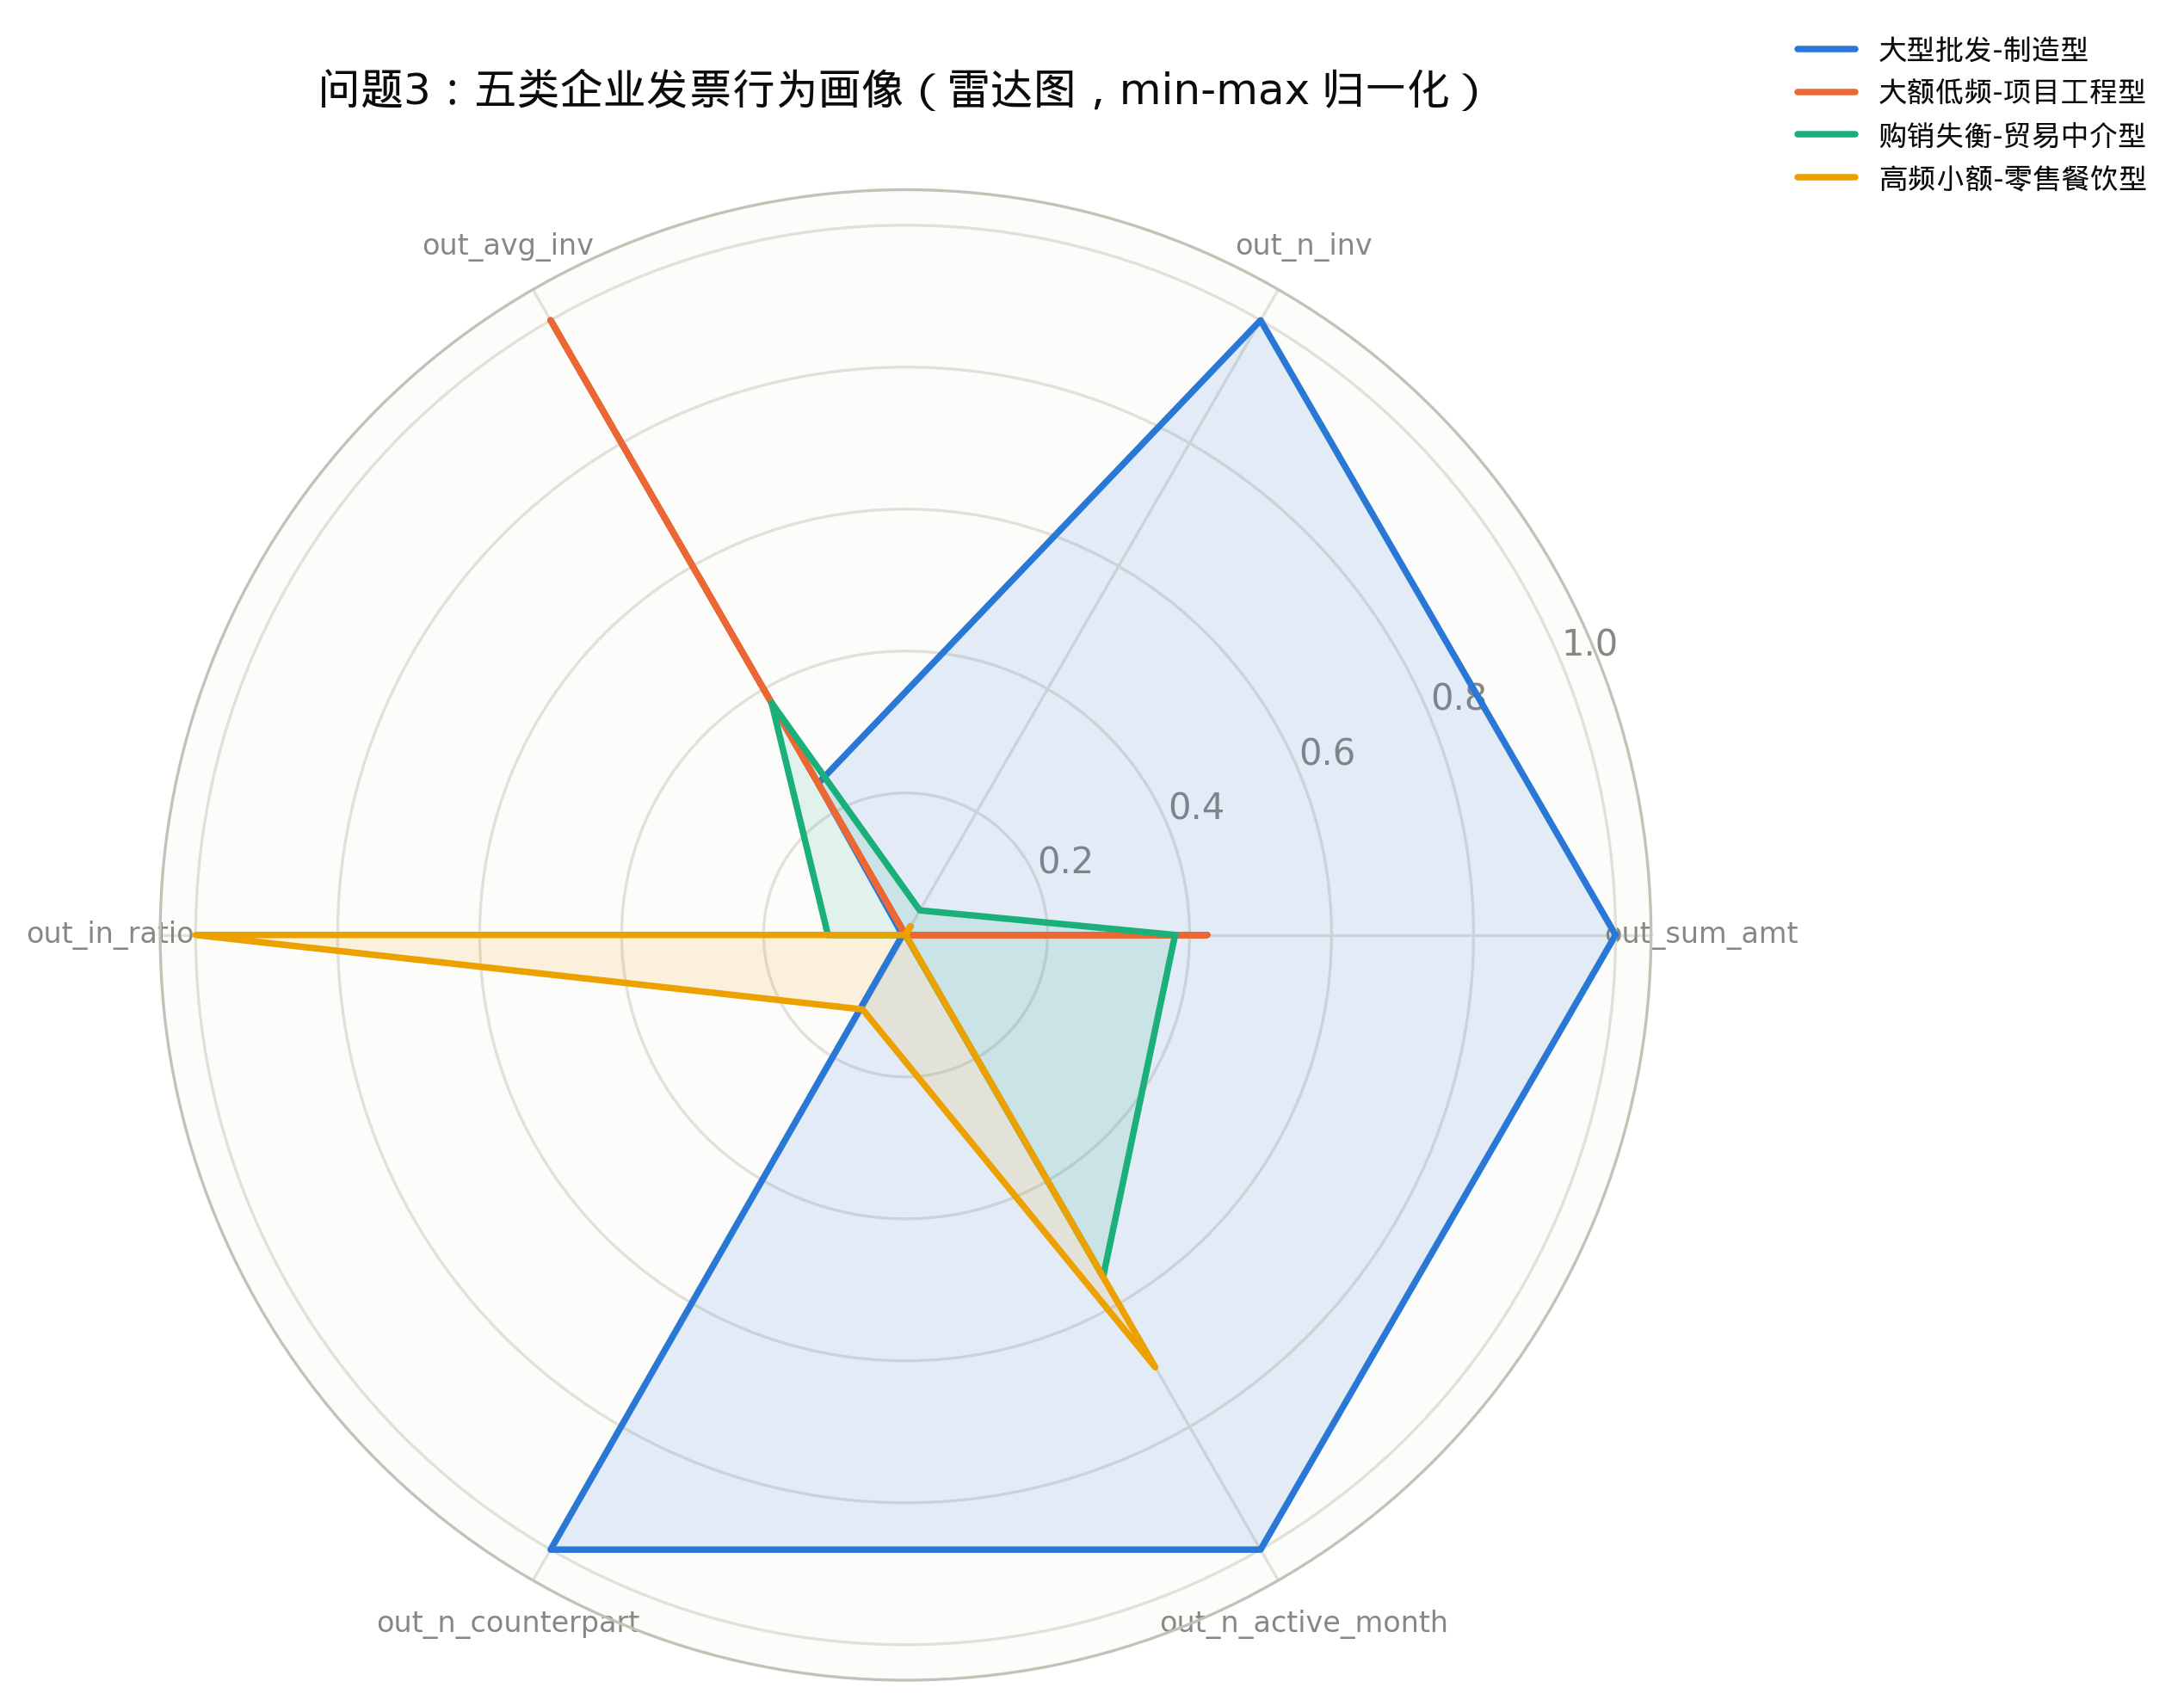
\includegraphics[width=\textwidth]{images/fig30_01_cluster_radar.png}
        \caption{四类企业行为画像雷达图}
        \label{fig:radar}
    \end{minipage}
    \hfill
    \begin{minipage}[t]{0.42\textwidth}
        \centering
        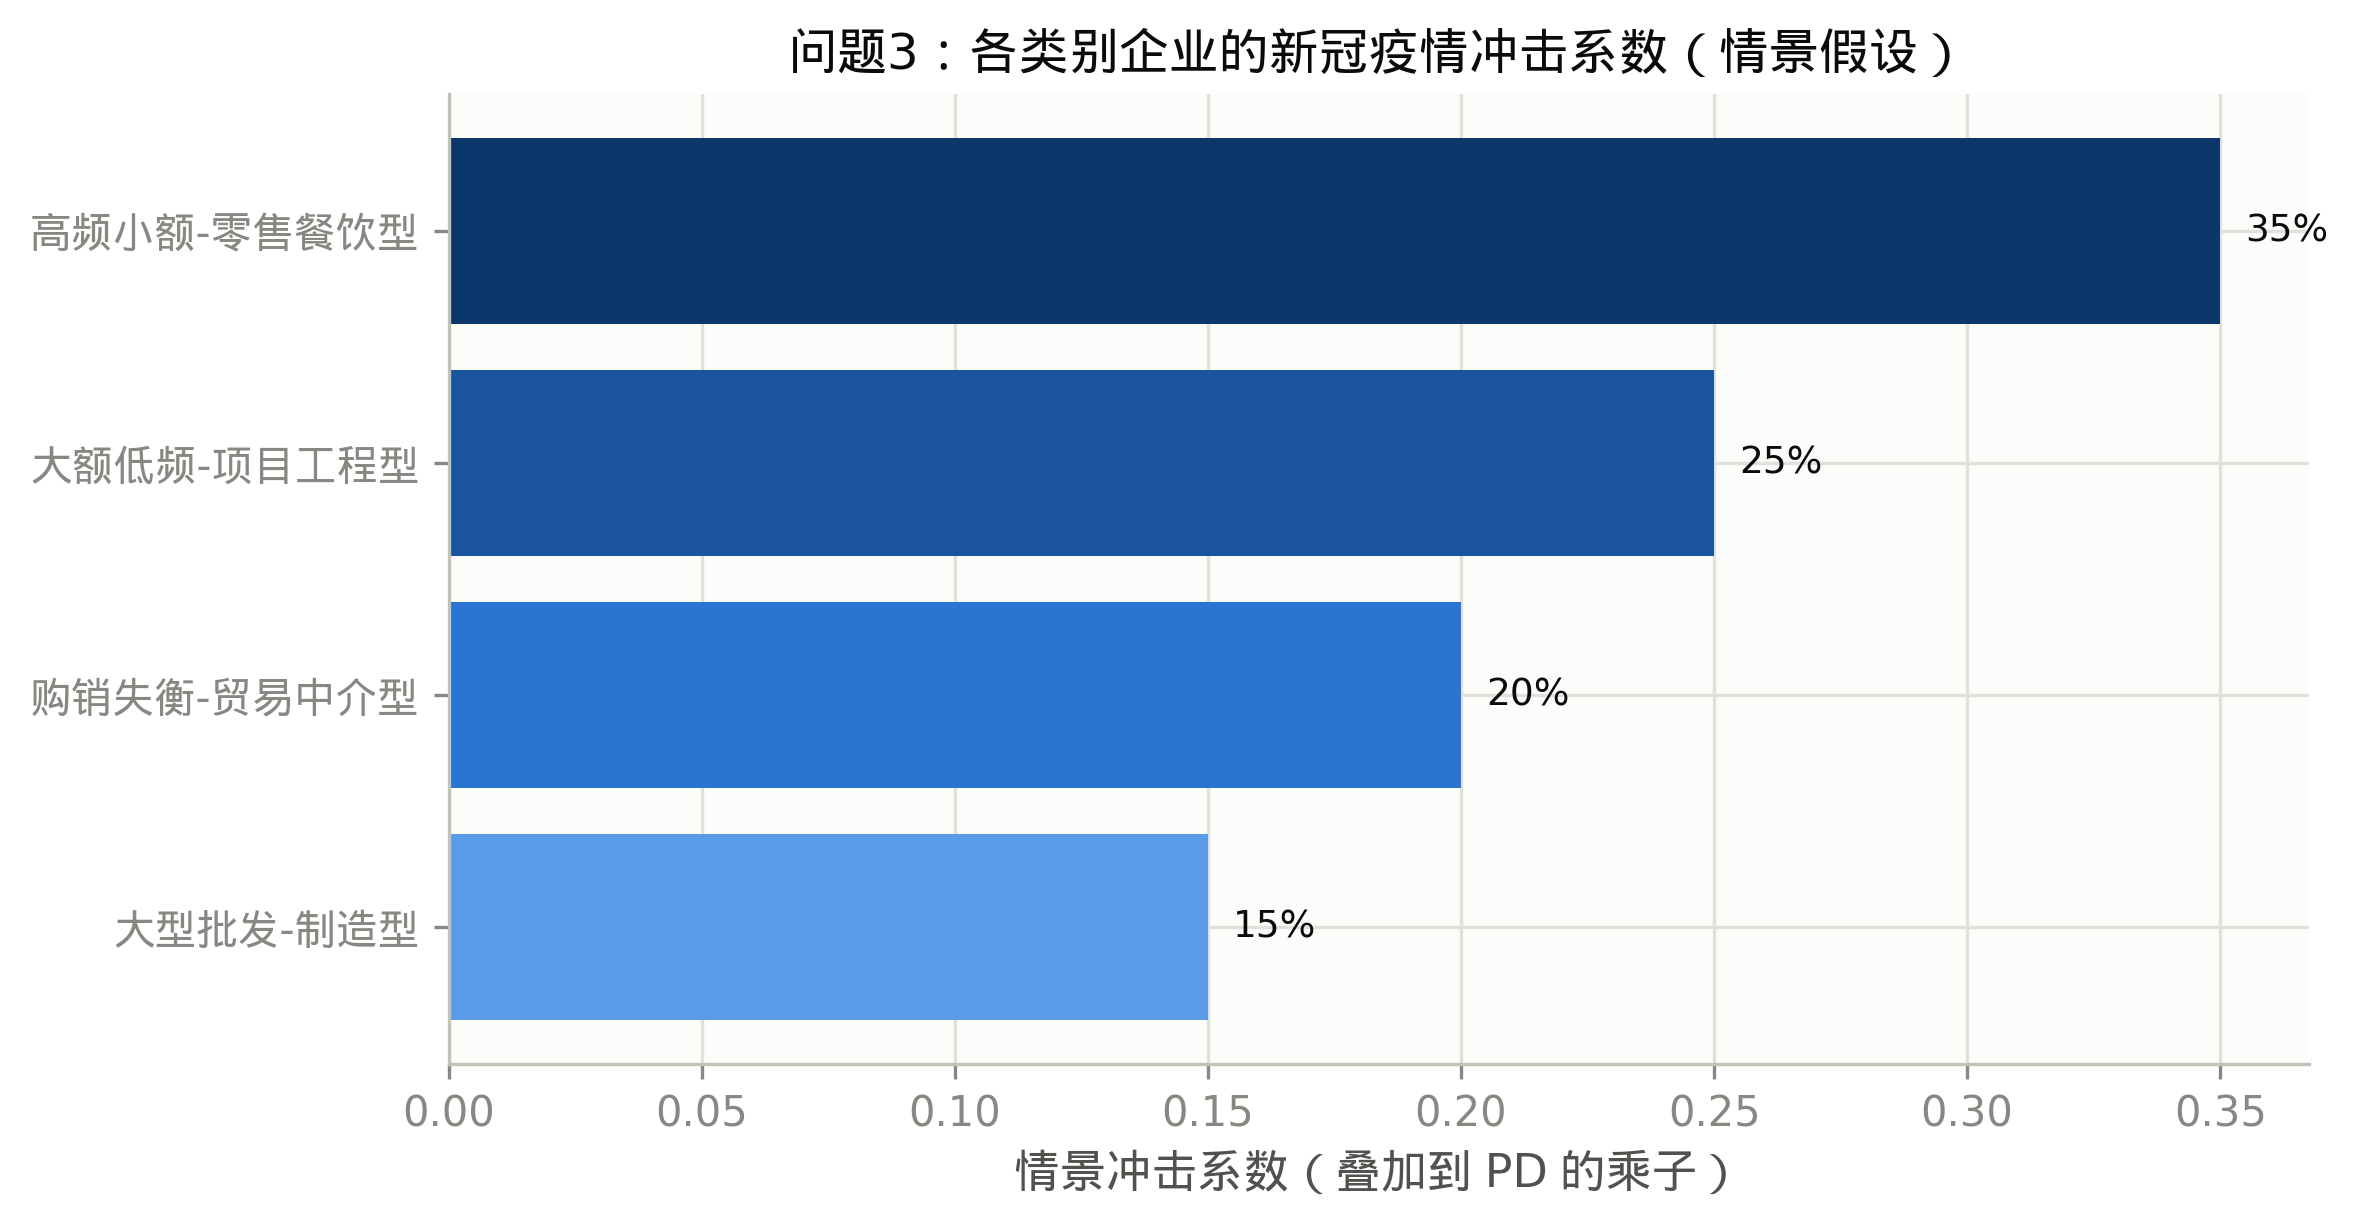
\includegraphics[width=\textwidth]{images/fig30_02_shock_multipliers.png}
        \caption{各类别情景冲击系数（按大小排序）}
        \label{fig:shock}
    \end{minipage}
\end{figure}

\subsubsection{冲击传导机制}

参照新冠疫情冲击下分行业信用压力的文献证据\cite{Banerjee2021,Wang2025}（住宿餐饮、零售等接触型服务行业承压最重，制造与批发相对有韧性），并结合类别画像设定情景冲击系数$\delta_k$（表~\ref{tab:cluster}、图~\ref{fig:shock}）：高频小额零售餐饮型0.35最高，大额低频项目工程型0.25（工程停工、作废率本已极高），贸易中介型0.20，大型批发制造型0.15。冲击沿两条渠道传导：

\begin{equation}
    \mathrm{PD}_i' = \min\left\{\mathrm{PD}_i\left(1+\delta_{k(i)}\right),\ 0.95\right\}, \qquad
    S_i' = S_i\left(1 - 0.5\,\delta_{k(i)}\right),
    \label{eq:shock}
\end{equation}

即违约概率按类别乘子上升、销项额（进而额度上限）按类别收缩。冲击后302家企业PD均值由0.188升至0.225（图~\ref{fig:pd_shift}），零售餐饮类PD中位数上升最显著。

\begin{figure}[H]
    \centering
    \begin{minipage}[t]{0.48\textwidth}
        \centering
        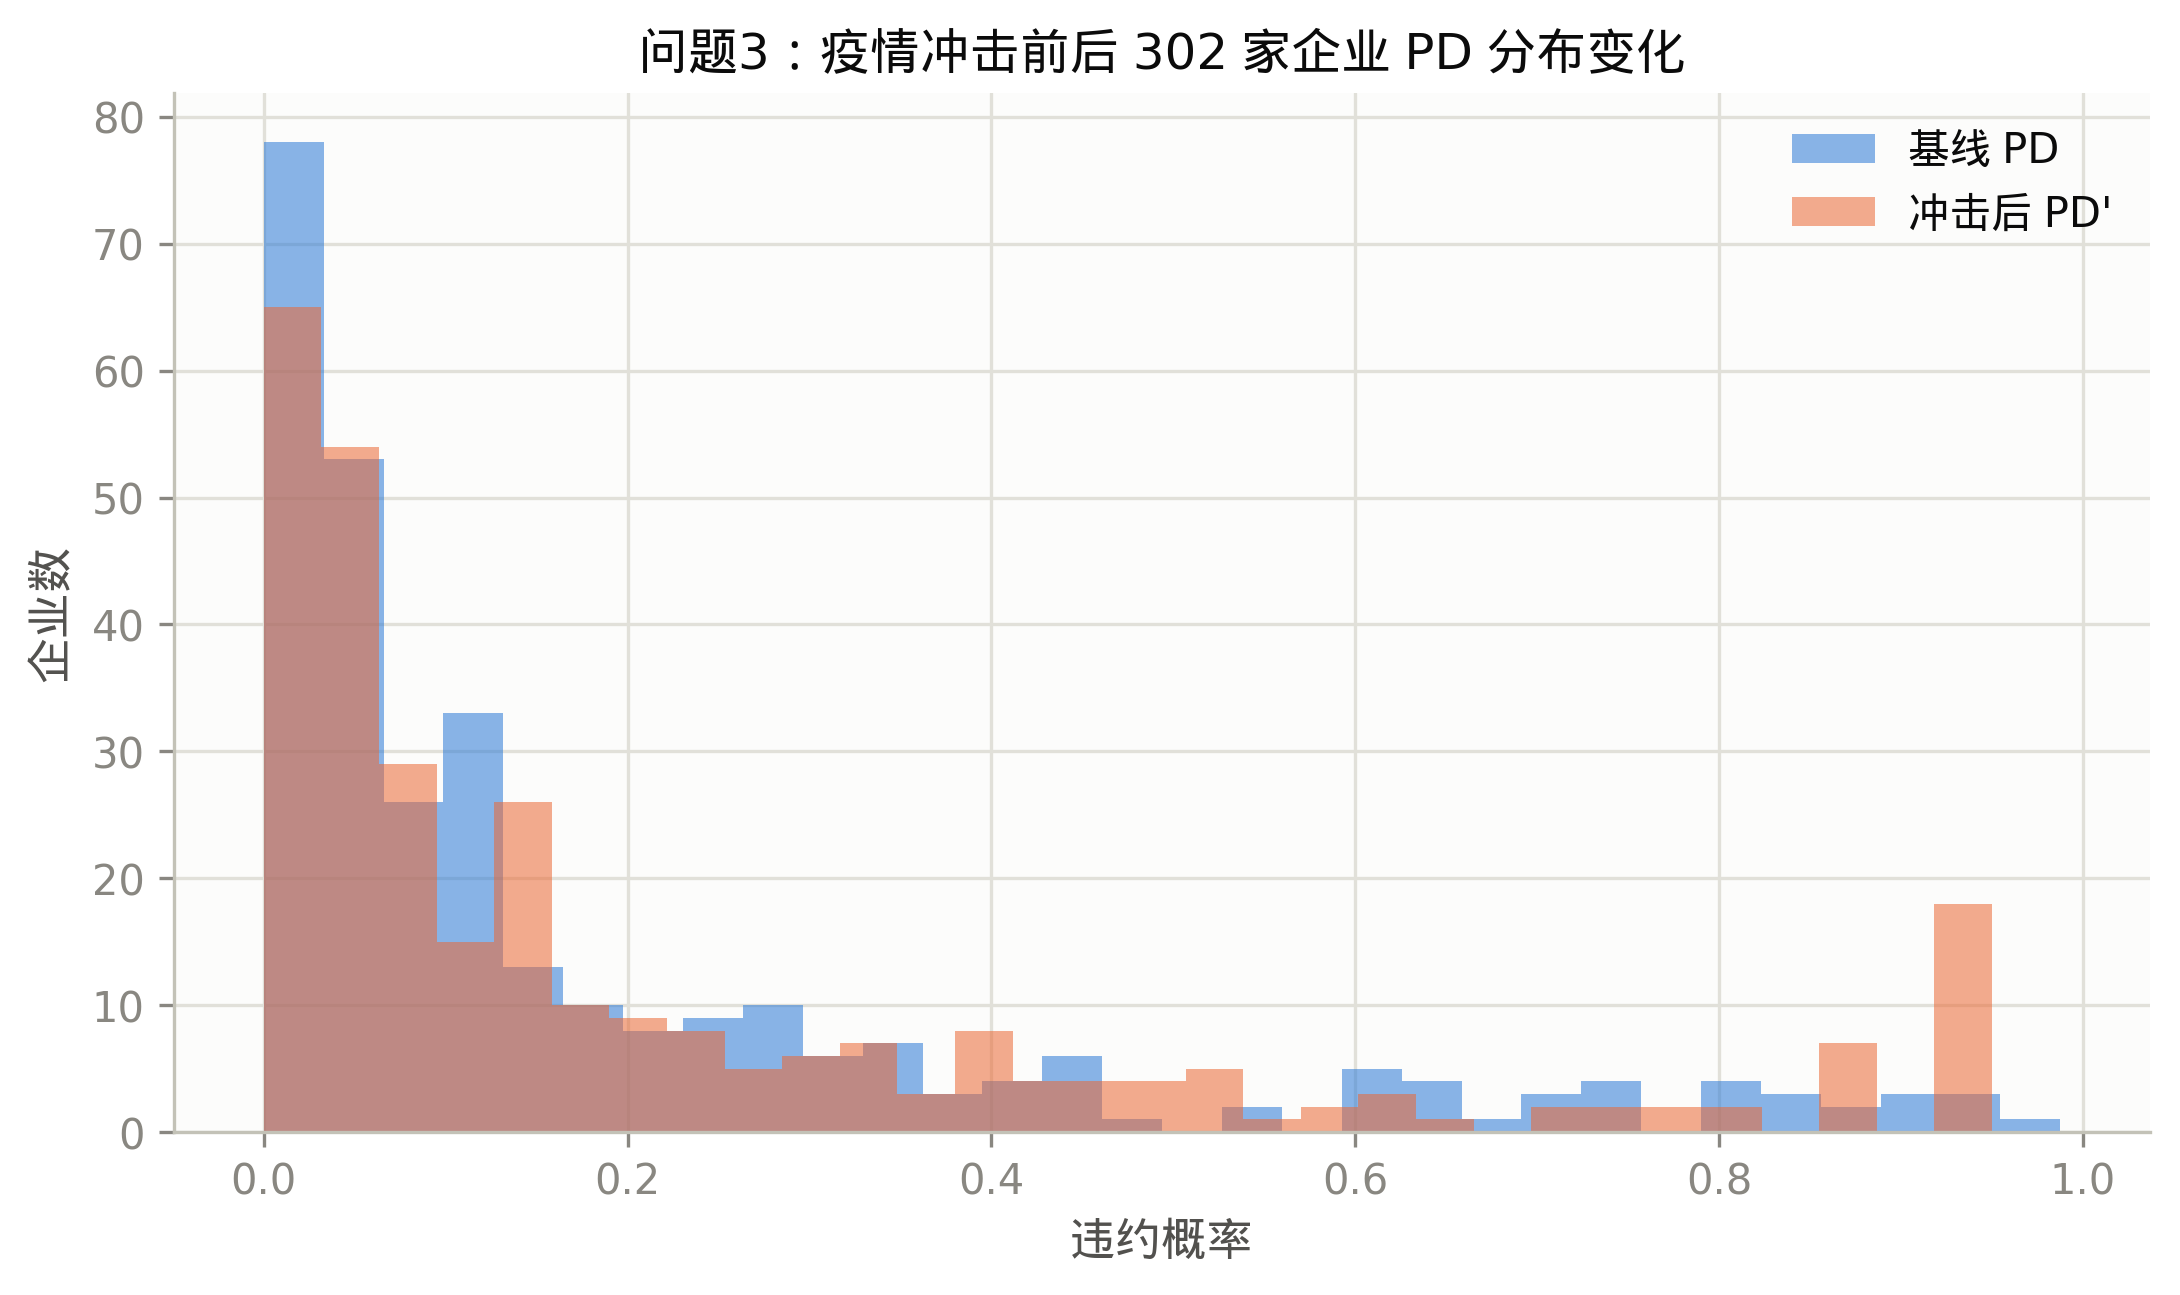
\includegraphics[width=\textwidth]{images/fig30_04_pd_shift.png}
        \caption{冲击前后PD分布变化}
        \label{fig:pd_shift}
    \end{minipage}
    \hfill
    \begin{minipage}[t]{0.48\textwidth}
        \centering
        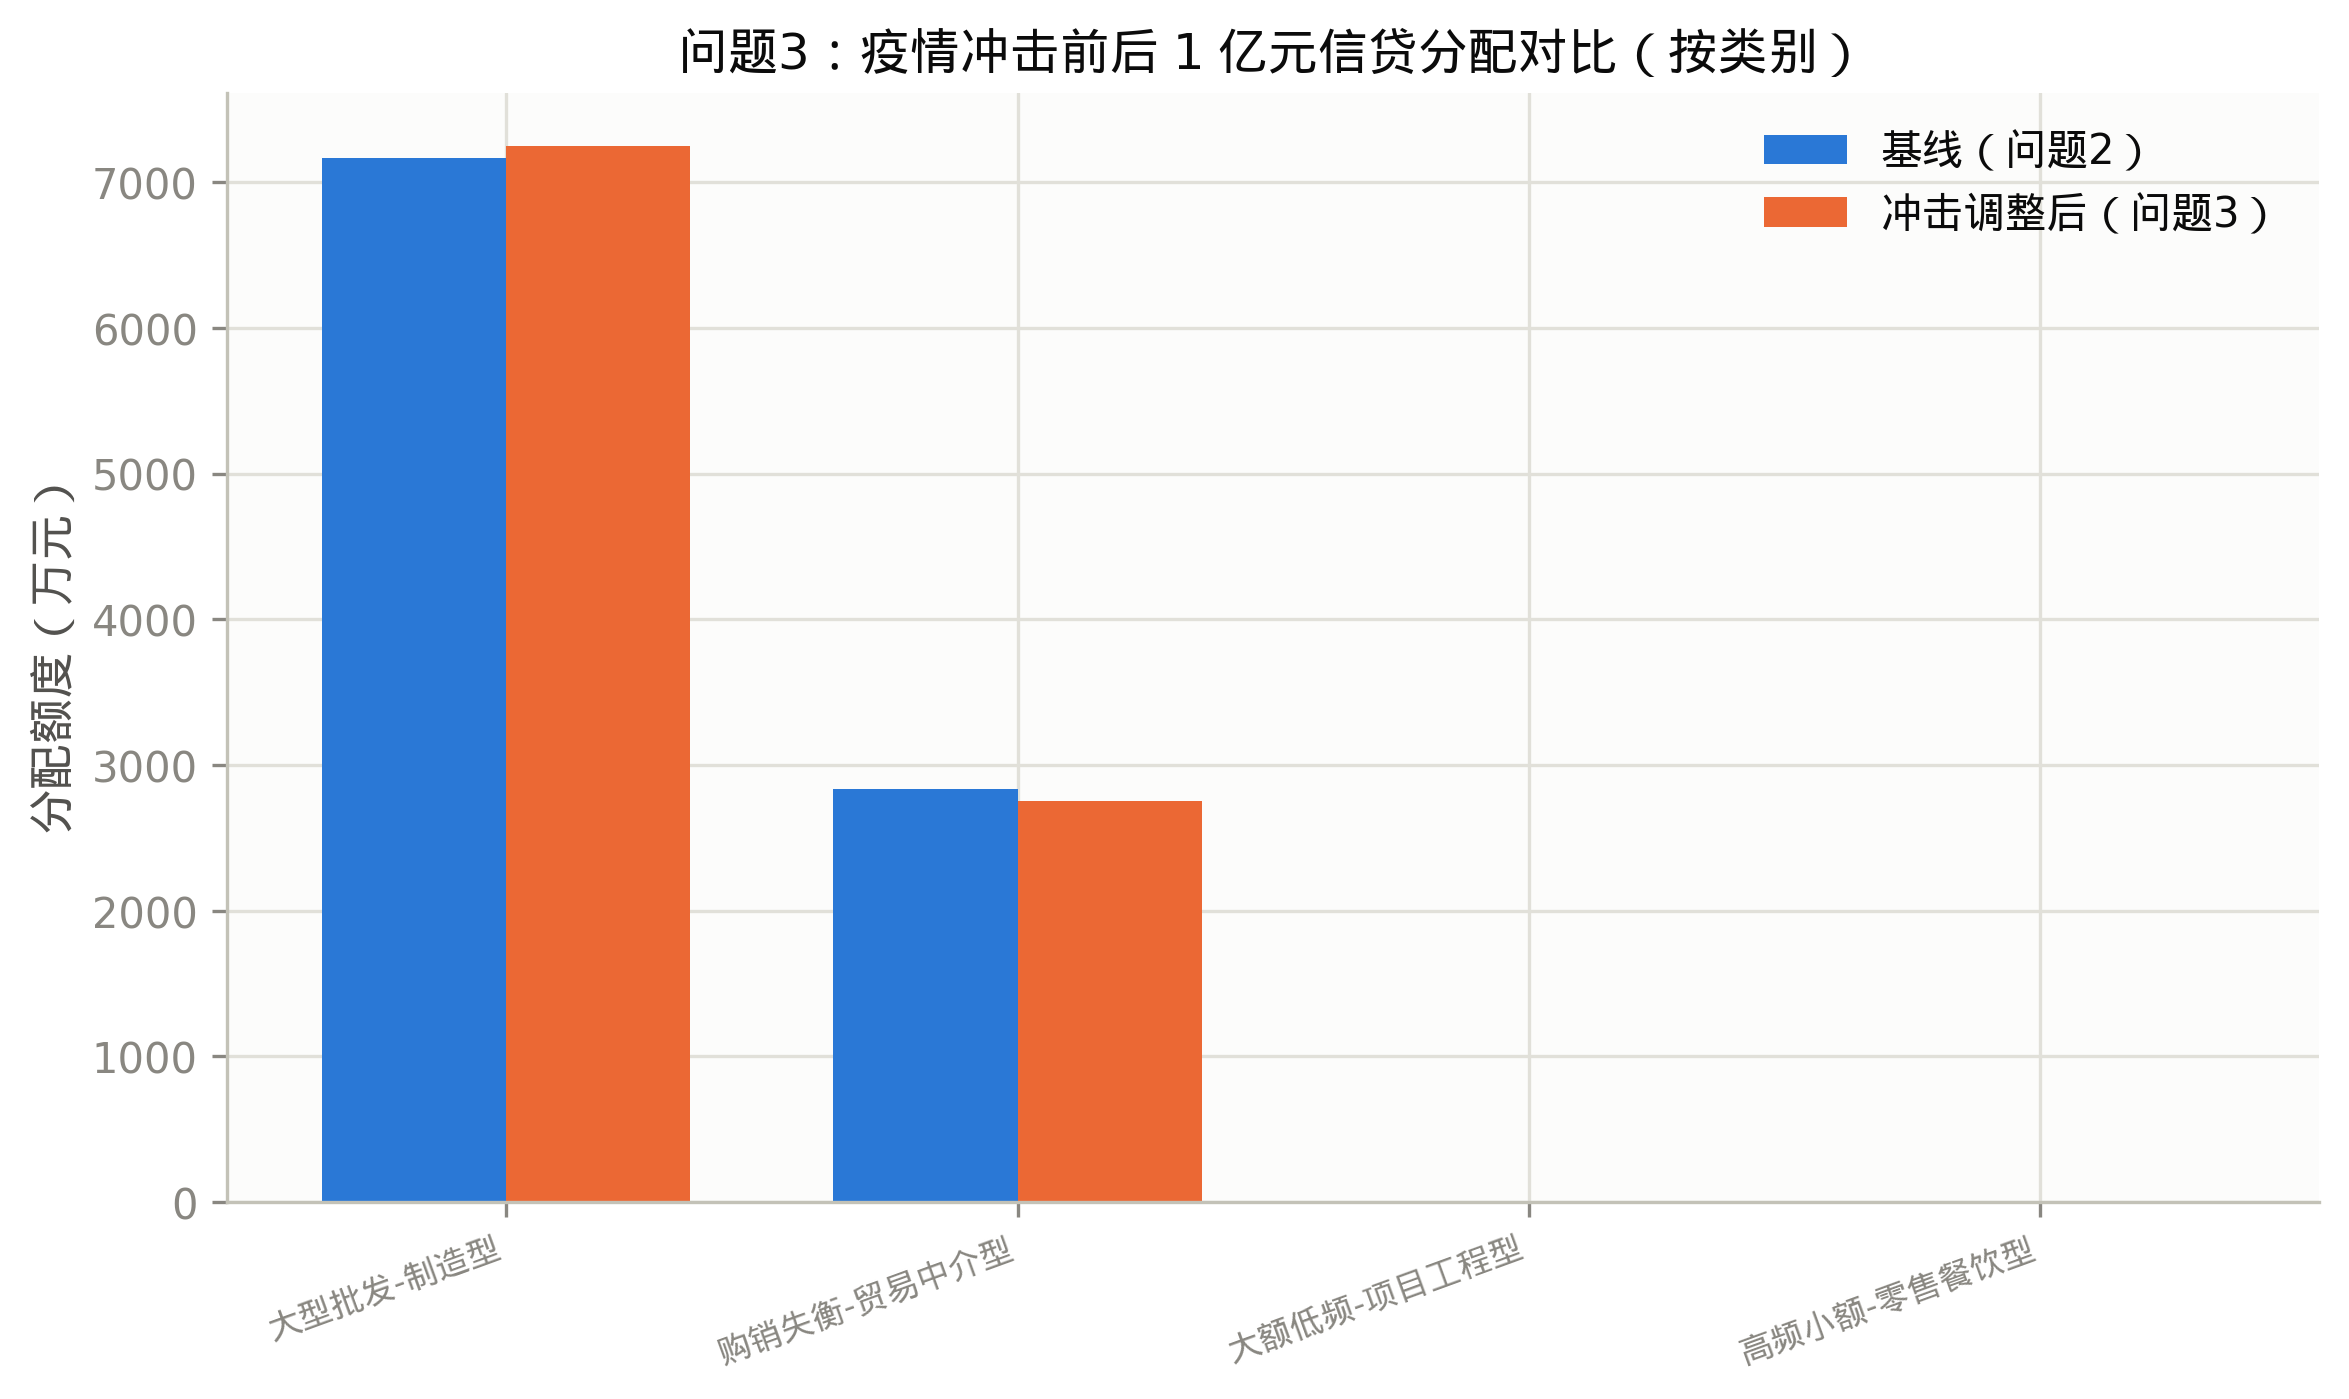
\includegraphics[width=\textwidth]{images/fig30_03_allocation_shift.png}
        \caption{冲击前后1亿元分配对比（按类别）}
        \label{fig:alloc_shift}
    \end{minipage}
\end{figure}

\subsubsection{1亿元调整策略}

以冲击后的PD$'$与收缩后销项额重新求解式\eqref{eq:alloc}（$T=10000$万元），得到调整策略：放贷12家，其中9家维持、2家收缩、1家加码。期望收益357万元，略高于基线的356万元——信贷资源向冲击后仍保持超低风险的企业集中。图~\ref{fig:alloc_shift}对比了冲击前后的分配：大型批发制造型额度由7164万元增至7248万元（相对抗冲击、略有加码），购销失衡贸易中介型由2836万元收缩至2752万元，零售餐饮与项目工程型保持不贷（冲击系数最高且原PD偏高）。调整策略的直观解读是：\textbf{突发因素下信贷资源应向冲击敏感度低、违约概率低的企业倾斜，对高冲击类别主动收缩敞口}，这与"信贷调整"的题意一致，也为银行提供了可量化的压力情景预案。

%% ==================== 7. 模型的分析与检验 ====================
\section{模型的分析与检验}

\subsection{灵敏度分析}

对6个关键假设做单参数上下扰动，以tornado图（灵敏度分析的标准呈现方式）展示对总期望收益与放贷家数的影响（图~\ref{fig:tornado}）。影响最大的是\textbf{信贷总额}：总额$\pm2000$万元时收益由290万元增至421万元，放贷家数由10家增至14家，近似线性（图~\ref{fig:profit_total}）。\textbf{客户流失率}假设的敏感性最高：缩放$0.5\times/1.5\times$时收益分别为777与347万元，说明流失率直接决定最优利率，属模型最敏感假设。\textbf{违约回收率}从0提高到0.4时收益增至373万元，影响中等；\textbf{冲击系数}缩放$0.5\times/1.5\times$时收益为352/344万元，影响有限——放贷主体本就是低PD企业，冲击后仍具吸引力。相比之下，\textbf{额度比例}$\theta$（0.15/0.35）与\textbf{分层阈值偏移}（$\pm20\%$）的影响接近零，因为额度主要由评级上限决定，而分层偏移不改变顶层放贷对象。

\begin{figure}[H]
    \centering
    \begin{minipage}[t]{0.49\textwidth}
        \centering
        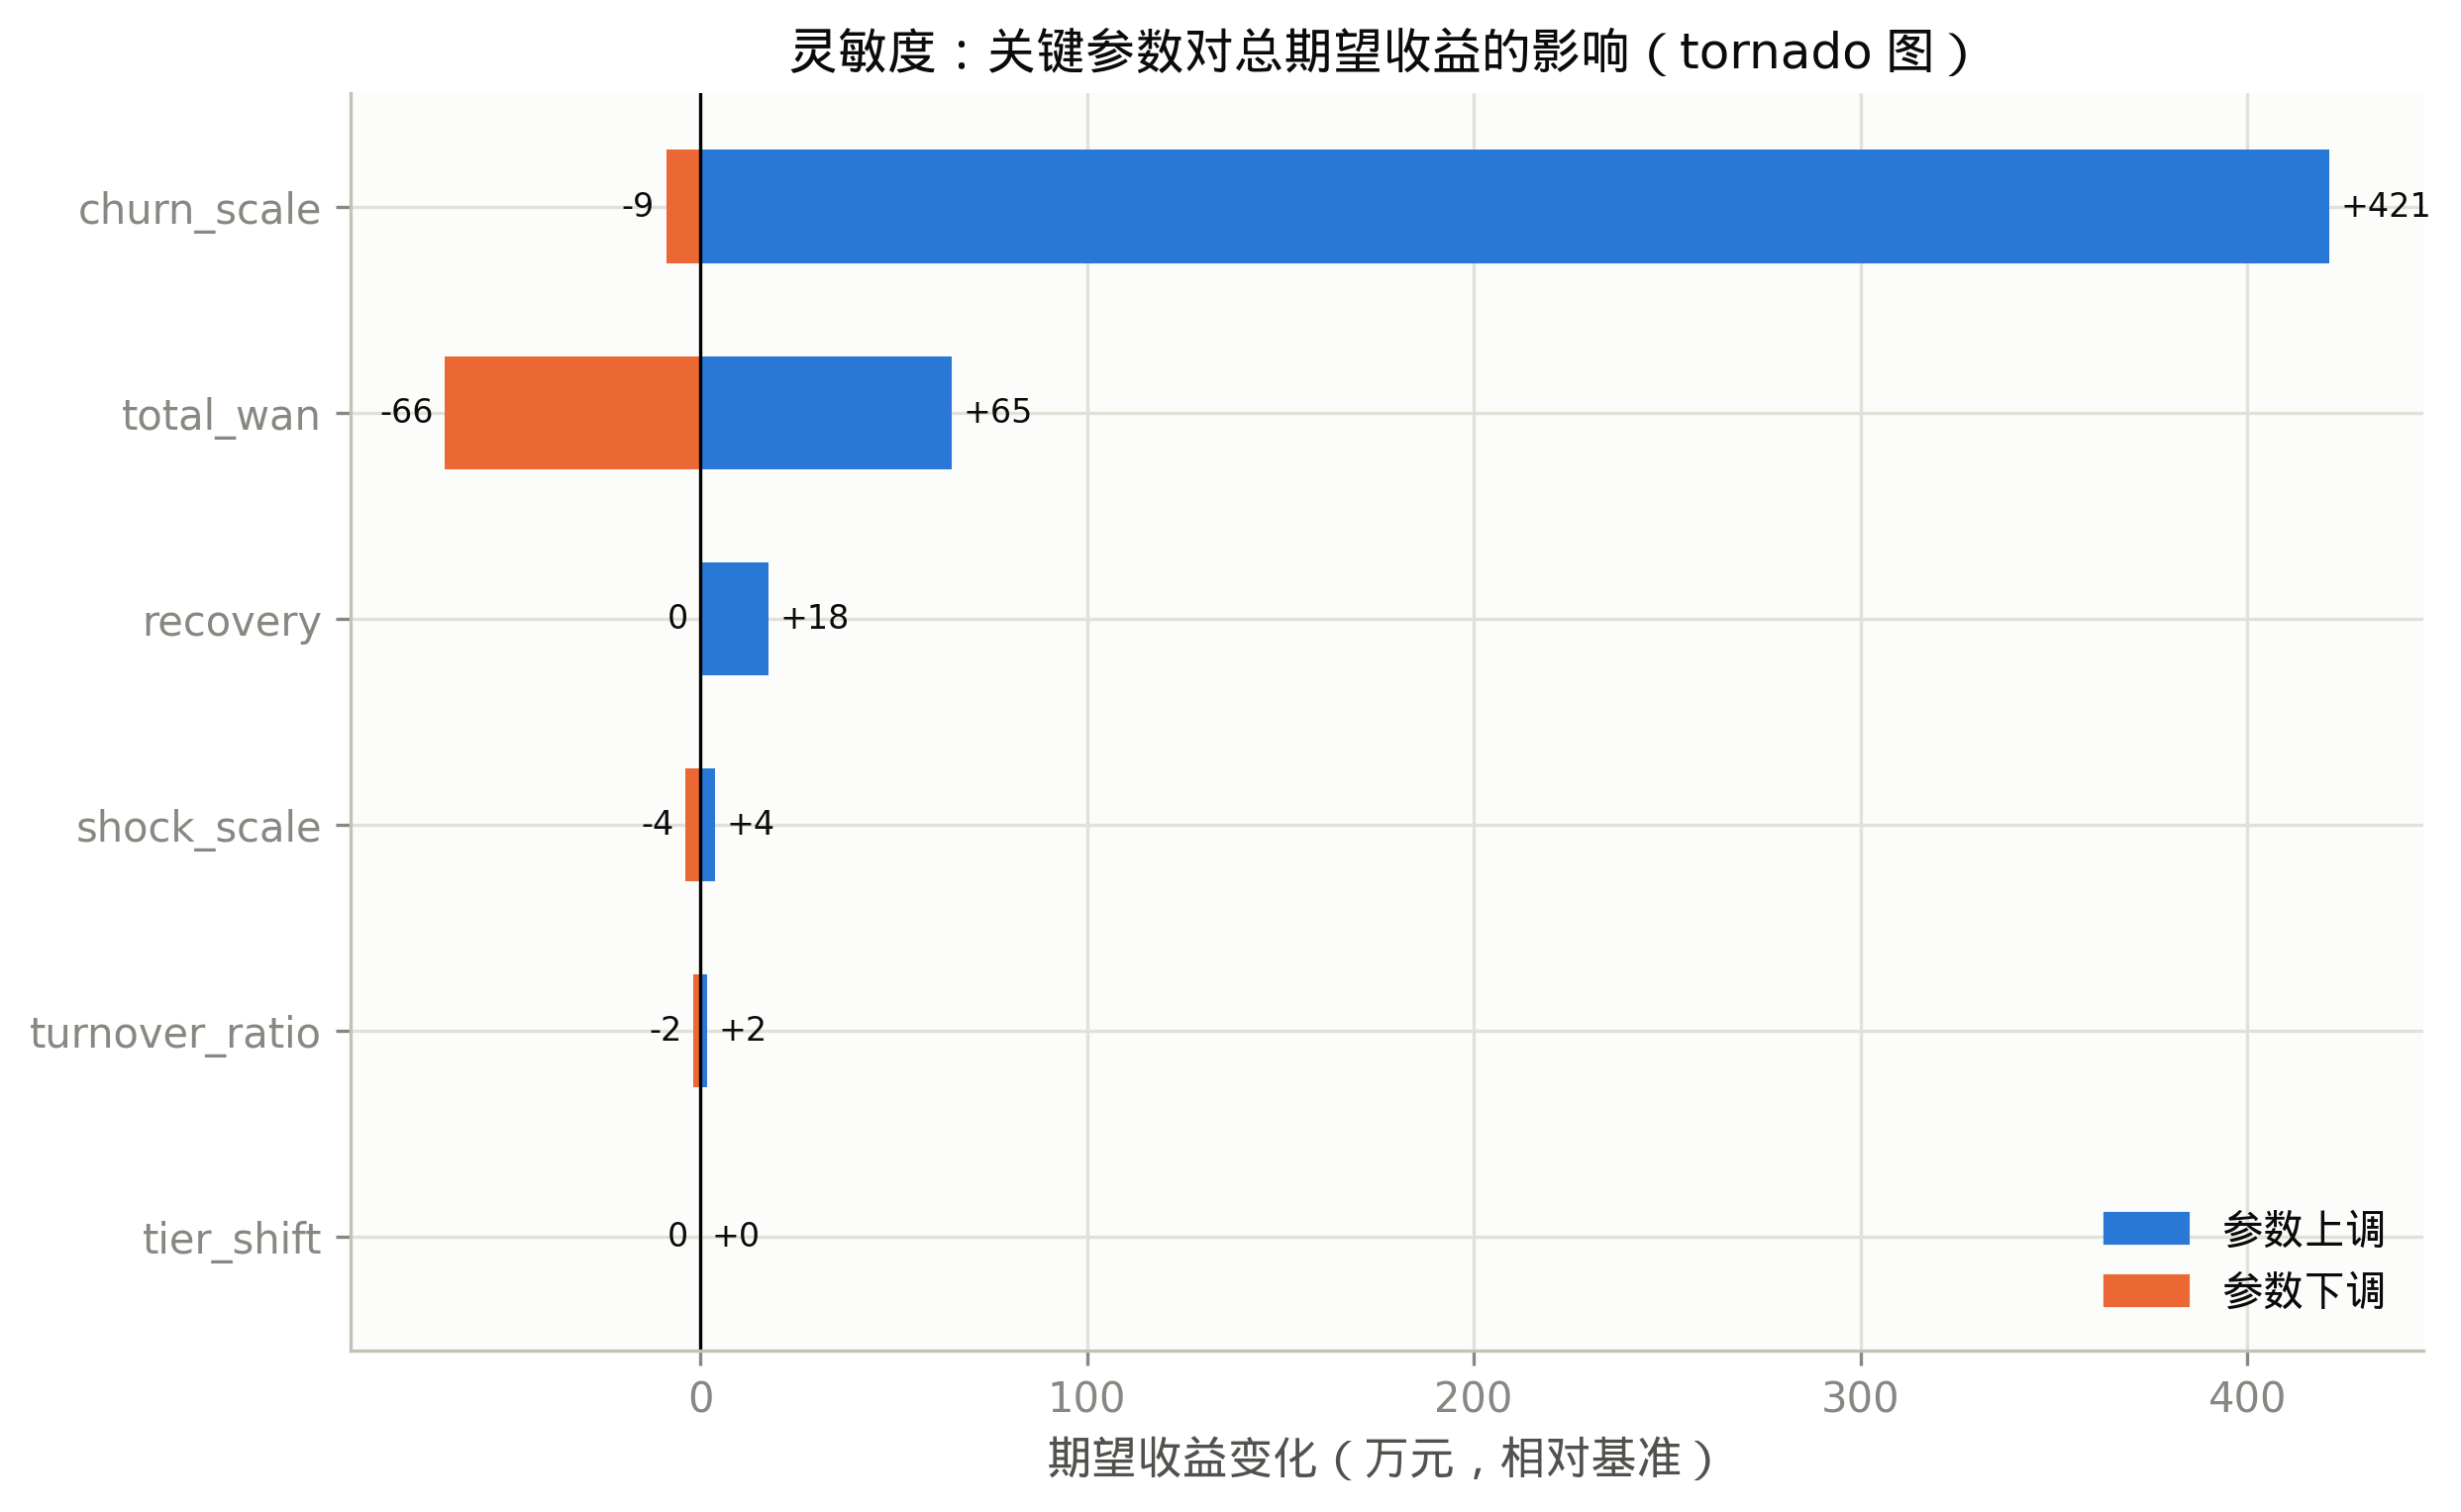
\includegraphics[width=\textwidth]{images/fig40_01_profit_tornado.png}
        \caption{总期望收益tornado图}
        \label{fig:tornado}
    \end{minipage}
    \hfill
    \begin{minipage}[t]{0.49\textwidth}
        \centering
        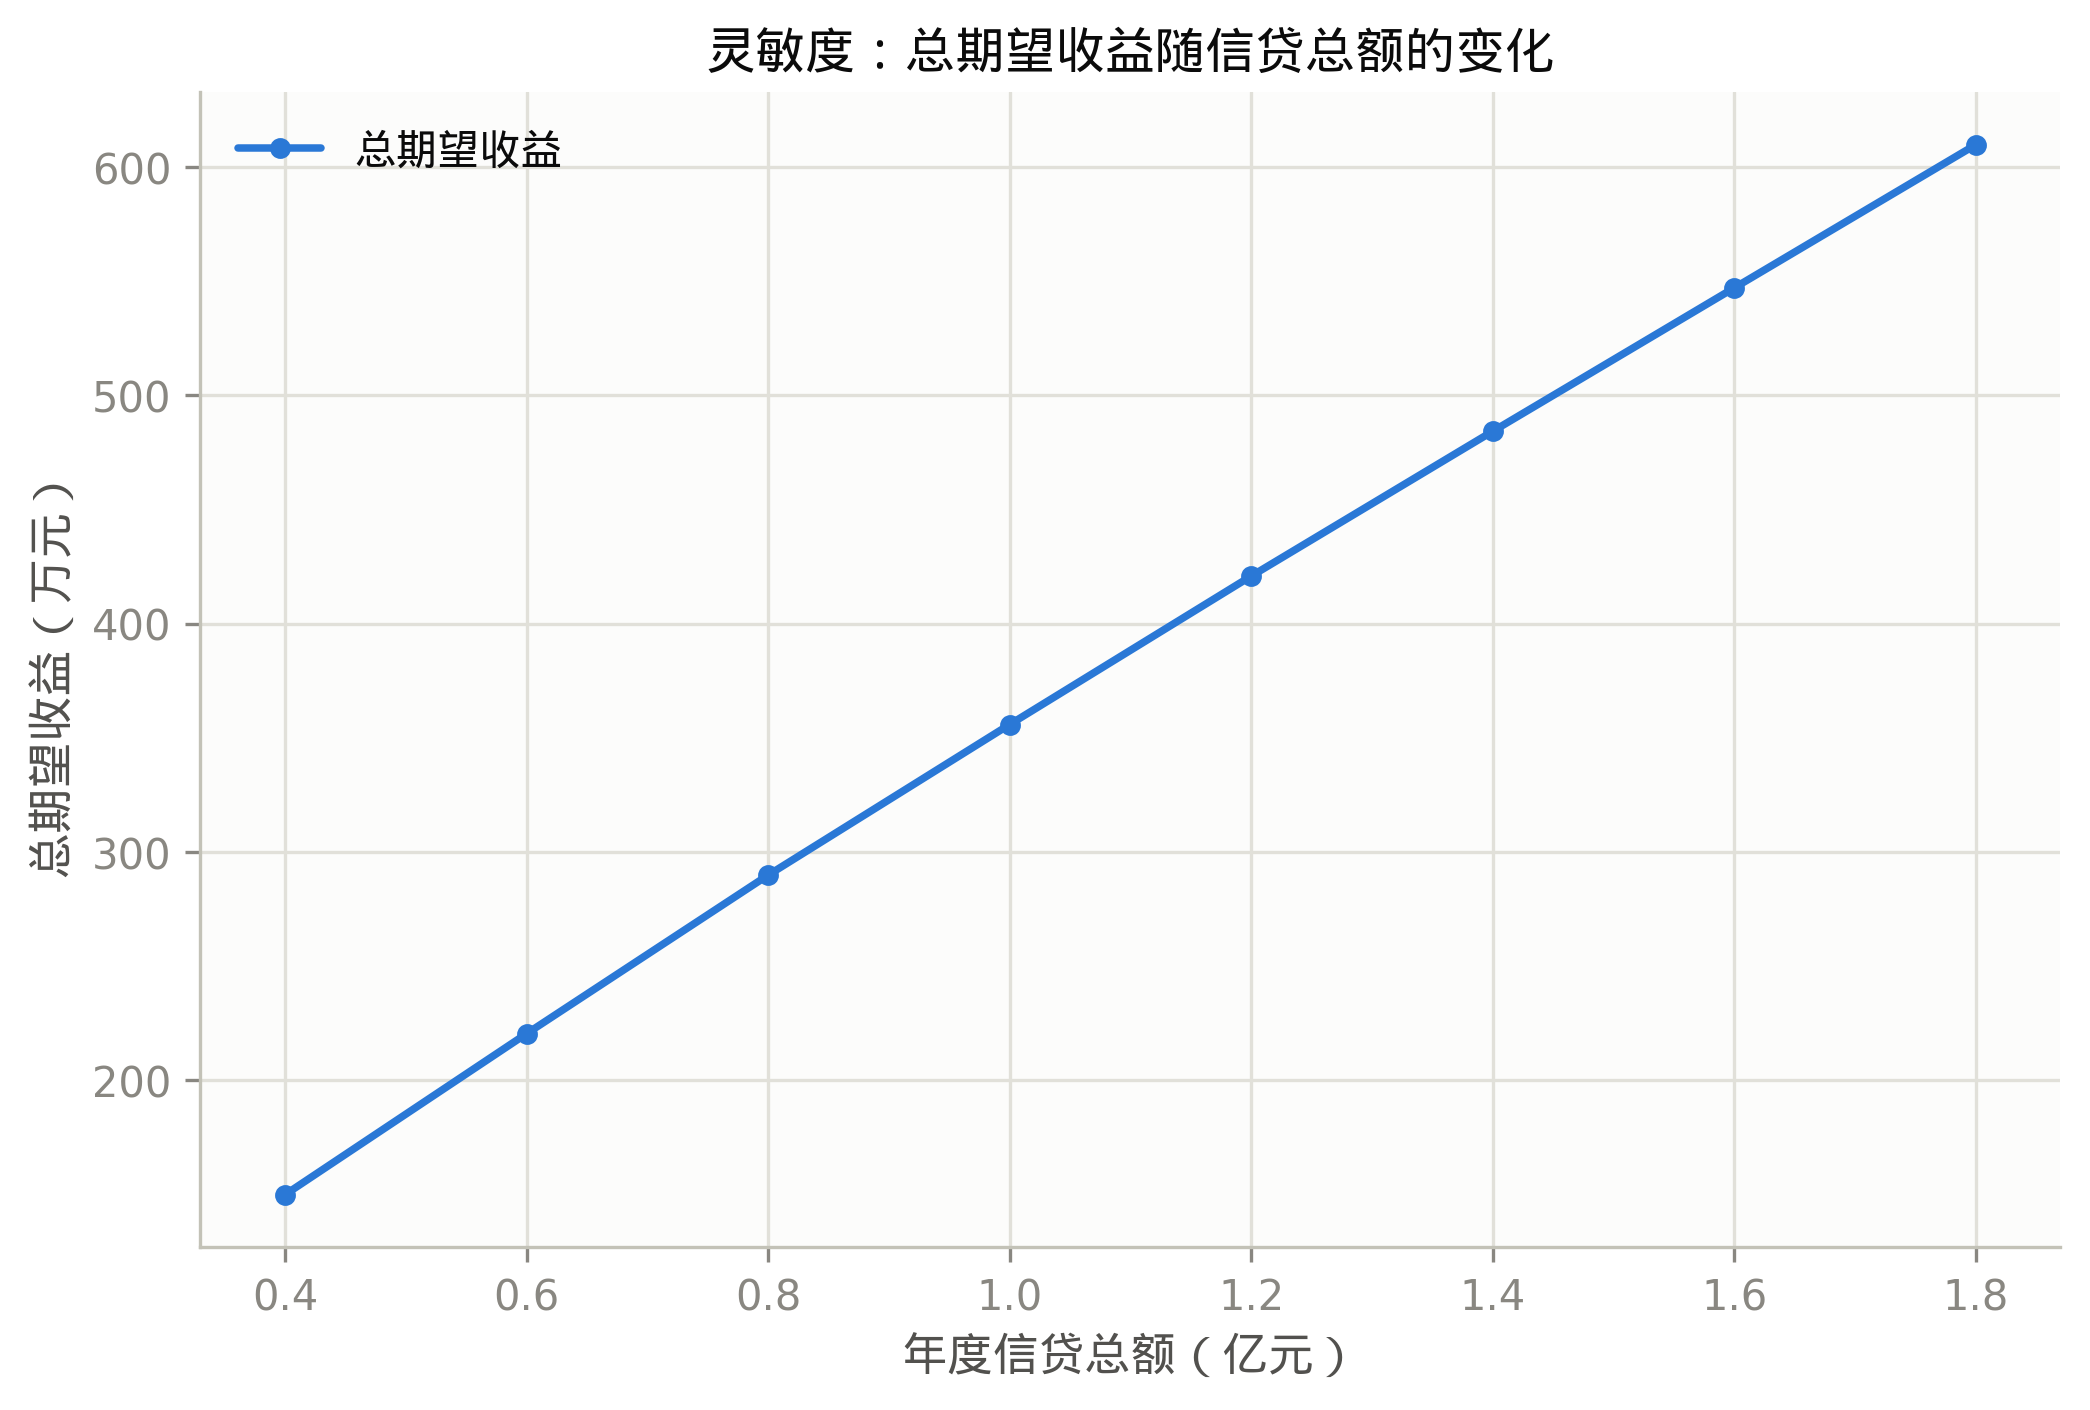
\includegraphics[width=\textwidth]{images/fig40_03_profit_vs_total.png}
        \caption{期望收益随信贷总额变化}
        \label{fig:profit_total}
    \end{minipage}
\end{figure}

结论：策略对信贷总额与流失率假设较敏感（影响收益绝对量），但对分层阈值、额度比例、冲击系数设定稳健（不改变放贷对象与方向性结论），模型结论可靠。表~\ref{tab:sens}~汇总了各参数扰动的数值结果。

\begin{table}[H]
\centering
\caption{灵敏度分析数值汇总（相对基准356万元）}
\label{tab:sens}
{\small
\begin{tabular}{lccc}
\toprule
\textbf{参数} & \textbf{下调} & \textbf{基准} & \textbf{上调} \\
\midrule
信贷总额（万元） & 8000：290 & 10000：356 & 12000：421 \\
客户流失率缩放 & 0.5$\times$：777 & 1.0$\times$：356 & 1.5$\times$：347 \\
违约回收率 & 0：356 & --- & 0.4：373 \\
冲击系数缩放 & 0.5$\times$：352 & 1.0$\times$：356 & 1.5$\times$：344 \\
额度比例$\theta$ & 0.15：354 & 0.25：356 & 0.35：357 \\
分层阈值偏移 & $-20\%$：356 & 0：356 & $+20\%$：356 \\
\bottomrule
\end{tabular}}
\end{table}

\subsection{模型验证}

按项目自证协议，三个子问题与灵敏度分析均执行了结构化验证，输出 \texttt{VERIFICATION REPORT} 并全部通过：

\begin{table}[H]
\centering
\caption{模型验证结果汇总}
\label{tab:verify}
{\footnotesize
\begin{tabular}{p{2.4cm}p{1.7cm}p{7.8cm}}
\toprule
\textbf{验证对象} & \textbf{通过/总数} & \textbf{代表性检查项} \\
\midrule
问题一模型 & 11/11 & AUC$>0.7$、PD按评级单调、$\rho>0.5$、利率$\in[4\%,15\%]$、D级不放贷、额度$\le$上限 \\
问题二模型 & 13/13 & 302家全覆盖、重算PD一致（$|\Delta|<10^{-9}$）、预算不超支、分层单调 \\
问题三模型 & 13/13 & 冲击传导重算一致、PD均值上升、调整动作与$\Delta$符号一致 \\
灵敏度分析 & 12/12 & 四组单调性方向正确、预算守恒、结果可复现 \\
\bottomrule
\end{tabular}}
\end{table}

此外，问题一模型用5折交叉验证评估判别力（AUC 0.935），避免了对训练集过拟合的误判；问题二以PSI量化迁移前提，并独立重算评分器输出与保存值核对（最大绝对误差$10^{-16}$量级）；问题三以重算校验冲击传导公式并逐项核对调整动作与额度变化的符号一致性，形成"训练—迁移—情景"全链路的验证闭环。全部验证脚本与结构化 \texttt{VERIFICATION REPORT} 均保留在项目 \texttt{src/verifications/} 与 \texttt{state/.tmp/} 目录中，保证论文中每个数值均可追溯到实际运行结果。

%% ==================== 8. 模型的评价、改进与推广 ====================
\section{模型的评价、改进与推广}

\subsection{模型优点}

\begin{enumerate}
    \item \textbf{数据驱动且可解释}：全部特征来自真实发票数据，逻辑回归直接输出违约概率并给出系数解释，优于黑箱模型；
    \item \textbf{可迁移}：评分器不依赖人工评级，天然适用于无标签样本，PSI检验保障迁移有效性；
    \item \textbf{策略可操作}：输出每家企业的放贷额度与利率，期望收益最大化目标与银行经营逻辑一致，贪心算法可扩展至任意总额；
    \item \textbf{情景化}：问题三将突发因素量化为类别冲击系数并给出调整动作，可直接支撑压力测试。
\end{enumerate}

\subsection{模型局限性}

\begin{enumerate}
    \item 附件1仅123家、27个违约样本，逻辑回归受小样本限制，特征选择可更系统（如逐步回归/LASSO）;
    \item 企业名称脱敏导致无法获取真实行业信息，问题三的类别是行为代理画像，冲击系数是文献校准的情景假设而非实测值;
    \item 1亿元预算下策略集中于约12家最优企业，未显式引入分散化（覆盖率）约束;
    \item 假设违约全额损失（$R=0$），未考虑抵押、担保等风险缓释手段。
\end{enumerate}

\subsection{改进方向与推广}

\begin{enumerate}
    \item \textbf{评分卡化}：将连续PD映射为整数评分卡，并引入LASSO/逐步回归做特征选择，提升可解释性与稳健性;
    \item \textbf{多期动态}：将单期静态分配扩展为滚动多期模型，允许额度在不同企业间动态调整;
    \item \textbf{约束增强}：在分配模型中增加覆盖率、行业集中度等约束，或引入均值-方差/鲁棒优化处理参数不确定性\cite{Torkian2025};
    \item \textbf{推广}：本框架可推广至供应链金融、个人消费信贷等"票据/流水驱动"的授信场景，只需替换特征与流失率曲线。
\end{enumerate}

%% ==================== 9. 参考文献 ====================
\section*{参考文献}
\addcontentsline{toc}{section}{参考文献}

\begin{thebibliography}{99}

\bibitem{Chen2024}
Chen B, Jin W, Lu H. Using a genetic backpropagation neural network model for credit risk assessment in the micro, small and medium-sized enterprises[J]. \textit{Heliyon}, 2024, 10: e33516. DOI: 10.1016/j.heliyon.2024.e33516.

\bibitem{Fahr2022}
Fáhr F, de Lima J D, Santos G D, Mazzioni S. Proposition of credit risk forecasting models for small and medium enterprises through logistic regression[J]. \textit{Gestão \& Regionalidade}, 2022, 38(113): 219-240.

\bibitem{Dickson2011}
Dickson J. On measures for illustrating credit risk assessments: the case of heat maps, risk matrices and cubes[C]. BIS IFC Bulletin No. 34, 2011.

\bibitem{Byanjankar2021}
Byanjankar A, Mezei J, Heikkilä M. Data-driven optimization of peer-to-peer lending portfolios based on the expected value framework[J]. \textit{Intelligent Systems in Accounting, Finance and Management}, 2021, 28(4). DOI: 10.1002/isaf.1490.

\bibitem{Torkian2025}
Torkian V, Bamdad S, Sarfaraz A H. Integrating AI and OR for investment decision-making in emerging digital lending businesses: a risk-return multi-objective optimization approach[J]. \textit{Journal of the Operational Research Society}, 2025. DOI: 10.1080/01605682.2025.2498652.

\bibitem{Banerjee2021}
Banerjee R, Mehrotra A, Zampolli F. How much stress could Covid put on corporate credit? Evidence using sectoral data[J]. \textit{BIS Quarterly Review}, 2021: 51-63.

\bibitem{Wang2025}
Wang L. Bank financing for SMEs in times of crisis: when "whatever-it-takes" confronts "black swans"[J]. \textit{Small Business Economics}, 2025, 65(2). DOI: 10.1007/s11187-025-01008-3.

\end{thebibliography}

%% ==================== 附录 ====================
\appendix
\section{核心代码}

以下代码为各模型源文件核心函数节选（用 \texttt{firstline}/\texttt{lastline} 从实际运行的源文件截取，与论文结果一一对应；完整源码见 \texttt{src/models/} 与 \texttt{src/verifications/}）。

\subsection{特征工程核心（\texttt{00\_data\_eda.py} 的 \texttt{enterprise\_features}）}

\lstinputlisting[style=pythonstyle, firstline=47, lastline=104,
  caption={enterprise\_features：发票数据向量化聚合（groupby+agg，无逐行循环）}]{../src/models/00_data_eda.py}

\subsection{问题一违约概率模型（\texttt{problem1\_credit.py} 的 \texttt{fit\_pd\_model}）}

\lstinputlisting[style=pythonstyle, firstline=73, lastline=101,
  caption={fit\_pd\_model：逻辑回归5折CV调参（完整文件另242行，含TOPSIS与策略分配）}]{../src/models/problem1_credit.py}

\subsection{问题一信贷分配（\texttt{problem1\_credit.py} 的 \texttt{build\_strategy}）}

\lstinputlisting[style=pythonstyle, firstline=156, lastline=187,
  caption={build\_strategy：利率-流失率权衡与线性背包贪心分配}]{../src/models/problem1_credit.py}

\subsection{问题二迁移打分与1亿元策略（\texttt{problem2\_credit.py} 的 \texttt{main} 前半）}

\lstinputlisting[style=pythonstyle, firstline=96, lastline=165,
  caption={problem2\_credit 主流程：迁移打分、PSI检验、伪评级分层与1亿元分配}]{../src/models/problem2_credit.py}

\subsection{问题三冲击分配（\texttt{problem3\_credit.py} 的 \texttt{allocate}）}

\lstinputlisting[style=pythonstyle, firstline=114, lastline=140,
  caption={allocate：冲击情景下按企业代号对齐额度上限的贪心分配}]{../src/models/problem3_credit.py}

\subsection{灵敏度分析核心（\texttt{sensitivity.py} 的 \texttt{run\_strategy}）}

\lstinputlisting[style=pythonstyle, firstline=74, lastline=127,
  caption={run\_strategy：参数化假设下的策略重算（支撑tornado图）}]{../src/models/sensitivity.py}

\end{document}
